\chapter{EKSPERIMEN DAN ANALISIS}

Bab ini menjelaskan mengenai implementasi dan prosedur pengujian algoritma estimasi, perbandingan hasil dari pengujian, dan analisis dari hasil tersebut.

\section{Skenario Pengujian}

Tujuan dari pengujian adalah untuk membandingkan kinerja dari algoritma estimasi yang dipilih dan mendapatkan algoritma estimasi yang paling baik dalam menyelesaikan masalah estimasi gerakan robot tim dan bola dalam kondisi latensi komunikasi.

Pengujian algoritma estimasi dilakukan di lingkungan simulasi yang dibangun pada \textit{framework} ROS yang dibahas di bab sebelumnya. \textit{Node-node} yang berfungsi untuk menjalankan simulasi dan estimasi yaitu \textit{node} simulasi \textit{world state}, simulasi sensor, \textit{world model}, dan simulasi komunikasi ditulis dalam bahasa C++17 yang di\textit{compile} menggunakan gcc dengan optimasi -O3, sedangkan \textit{node} aggregator dan evaluator yang bertugas untuk mengagregasi dan mengambil statistik dari data, beserta melakukan visualisasi ditulis dalam bahasa Python 3 menggunakan \textit{library} matplotlib. Beberapa \textit{node} tambahan juga digunakan seperti \textit{node} \textit{timer} untuk menyelesaikan simulasi setelah waktu tertentu, dan \textit{node} untuk menyimpan konfigurasi dan merekam eksekusi simulasi agar simulasi dapat ditampilkan ulang.

Berikut adalah spesifikasi \textit{hardware} yang digunakan dalam pengujian di lingkungan simulasi:
\begin{enumerate}
    \item OS Ubuntu 20.04.3 LTS
    \item CPU Intel(R) Core(TM) i7-9750H CPU @ 2.60GHz (12 CPUs)
    \item RAM 16 GB
\end{enumerate}

Pengujian dilakukan dengan mengambil statistik metrik \textit{error} berupa jarak dari estimasi masing-masing robot dibandingkan dengan \textit{world state} yang sesungguhnya. Masing-masing jenis \textit{world model} dijalankan sebanyak lima kali tiga menit waktu berjalannya program, sehingga didapatkan sekitar $5 \times 3 \times 60 \times 1000 : 30 = 30000$ banyak nilai per statistik yang akan dianalisis menggunakan ringkasan lima angkanya dan statistik lain seperti rata-rata.

Skenario pengujian dapat dijalankan dalam tiga jenis kondisi jaringan, yaitu:
\begin{enumerate}
    \item Kondisi baik dengan $80\%$ keadaan jaringan baik
    \item Kondisi sedang dengan $50\%$ keadaan jaringan baik
    \item Kondisi buruk dengan $20\%$ keadaan jaringan baik
\end{enumerate}

Untuk perbandingan kinerja algoritma, diiterasi beberapa jenis \textit{node} \textit{world model} dengan variasi algoritma estimasi yang berbeda-beda dengan iterasi sebelumnya:
\begin{enumerate}
    \item \textit{world model} O dimana lokalisasi dan estimasi dilakukan dengan naif
    \item \textit{world model} P yang melakukan lokalisasi dengan penapis partikel \textit{pose} dan estimasi bola menggunakan penapis Kalman
    \item \textit{world model} Q yang melakukan lokalisasi dengan penapis partikel \textit{pose} dan \textit{twist}
    \item \textit{world model} R yang mengestimasi bola menggunakan penapis partikel
    \item \textit{world model} RB yang tidak melakukan penyesuaian waktu saat mengirimkan hasil estimasi
    \item \textit{world model} S yang mengestimasi bola dengan OOSM-PF
    \item \textit{world model} SB yang mengestimasi bola dengan OOSM-PF dengan data opsional
    \item \textit{world model} SC yang mengestimasi bola dengan OOSM-KF
    \item \textit{world model} SD yang mengestimasi bola dengan OOSM-KF dengan data kombinasi
    \item \textit{world model} T yang mengoreksi lokasi teman menggunakan data \textit{vision}
\end{enumerate}

\section{Pengujian dan Analisis Algoritma Estimasi Dasar}

\subsection{Perbandingan Algoritma tanpa Penapis dan dengan Penapis}

\textit{World model} O yang melakukan lokalisasi dengan naif dengan mengakumulasi nilai odometri tanpa koreksi \textit{vision} dan menggunakan data persepsi bola dengan mentah dibuat sebagai pembanding paling dasar dengan algoritma dengan penapis sederhana.

\textit{World model} P menggunakan penapis partikel berbasis \textit{pose} untuk lokalisasinya dan penapis Kalman untuk mengestimasi posisi bola. Data dari teman digunakan secara mentah dan data bola dimasukan ke dalam penapis apabila \textit{timestamp}nya lebih baru. Dilakukan penyesuaian waktu dari \textit{timestamp} data ke waktu saat ini saat hasil estimasi objek dikirimkan.

\begin{figure}[p]
    \centering
    \medskip
    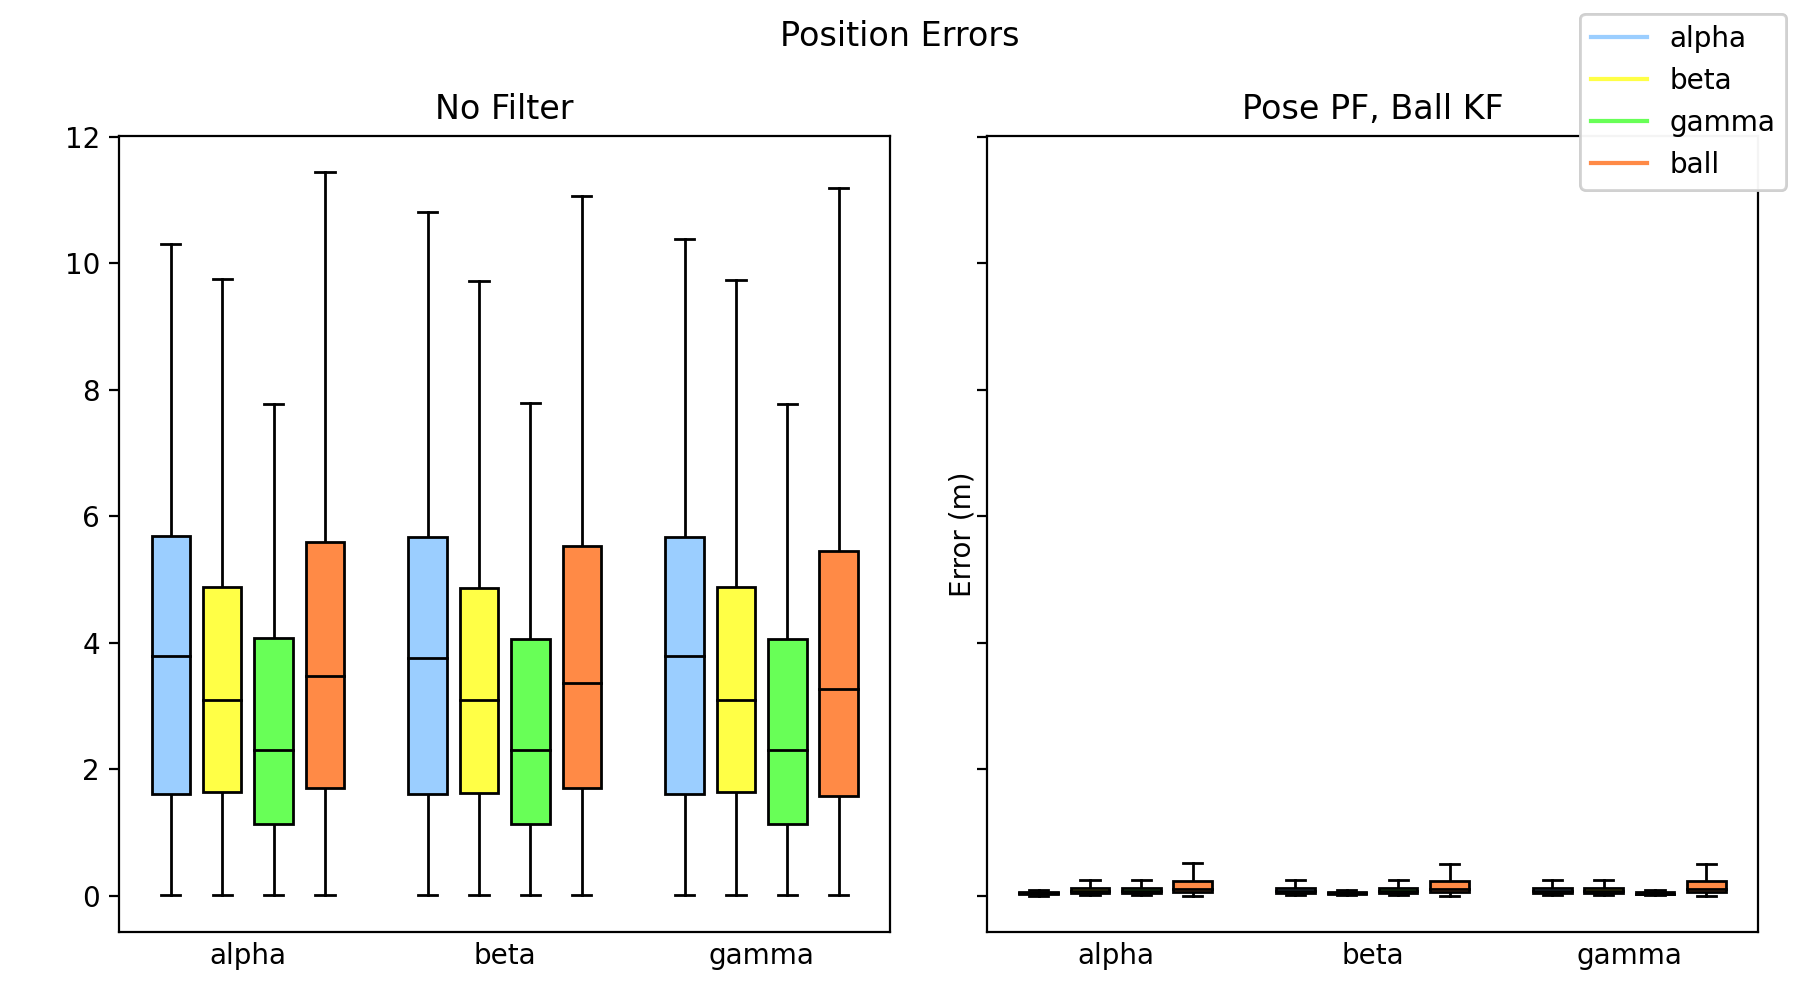
\includegraphics[width=0.9\textwidth]{resources/cfg1_AO_AP_error_pos.png}
    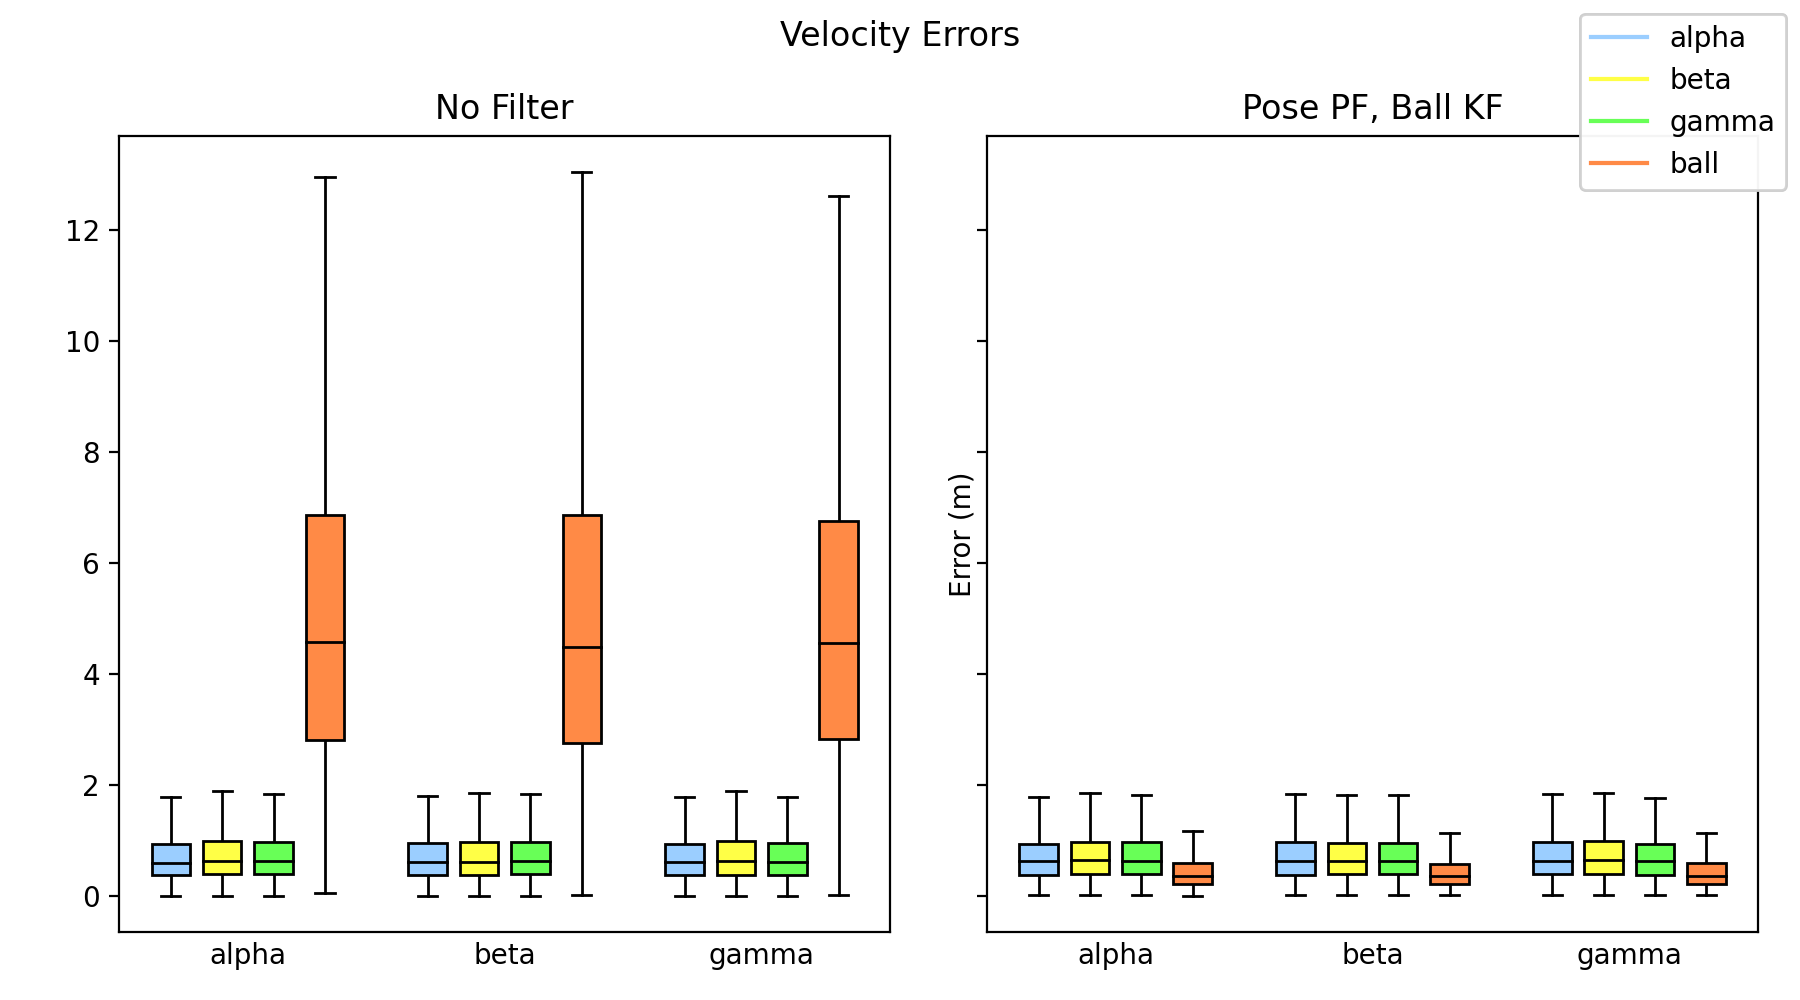
\includegraphics[width=0.9\textwidth]{resources/cfg1_AO_AP_error_vel.png}
    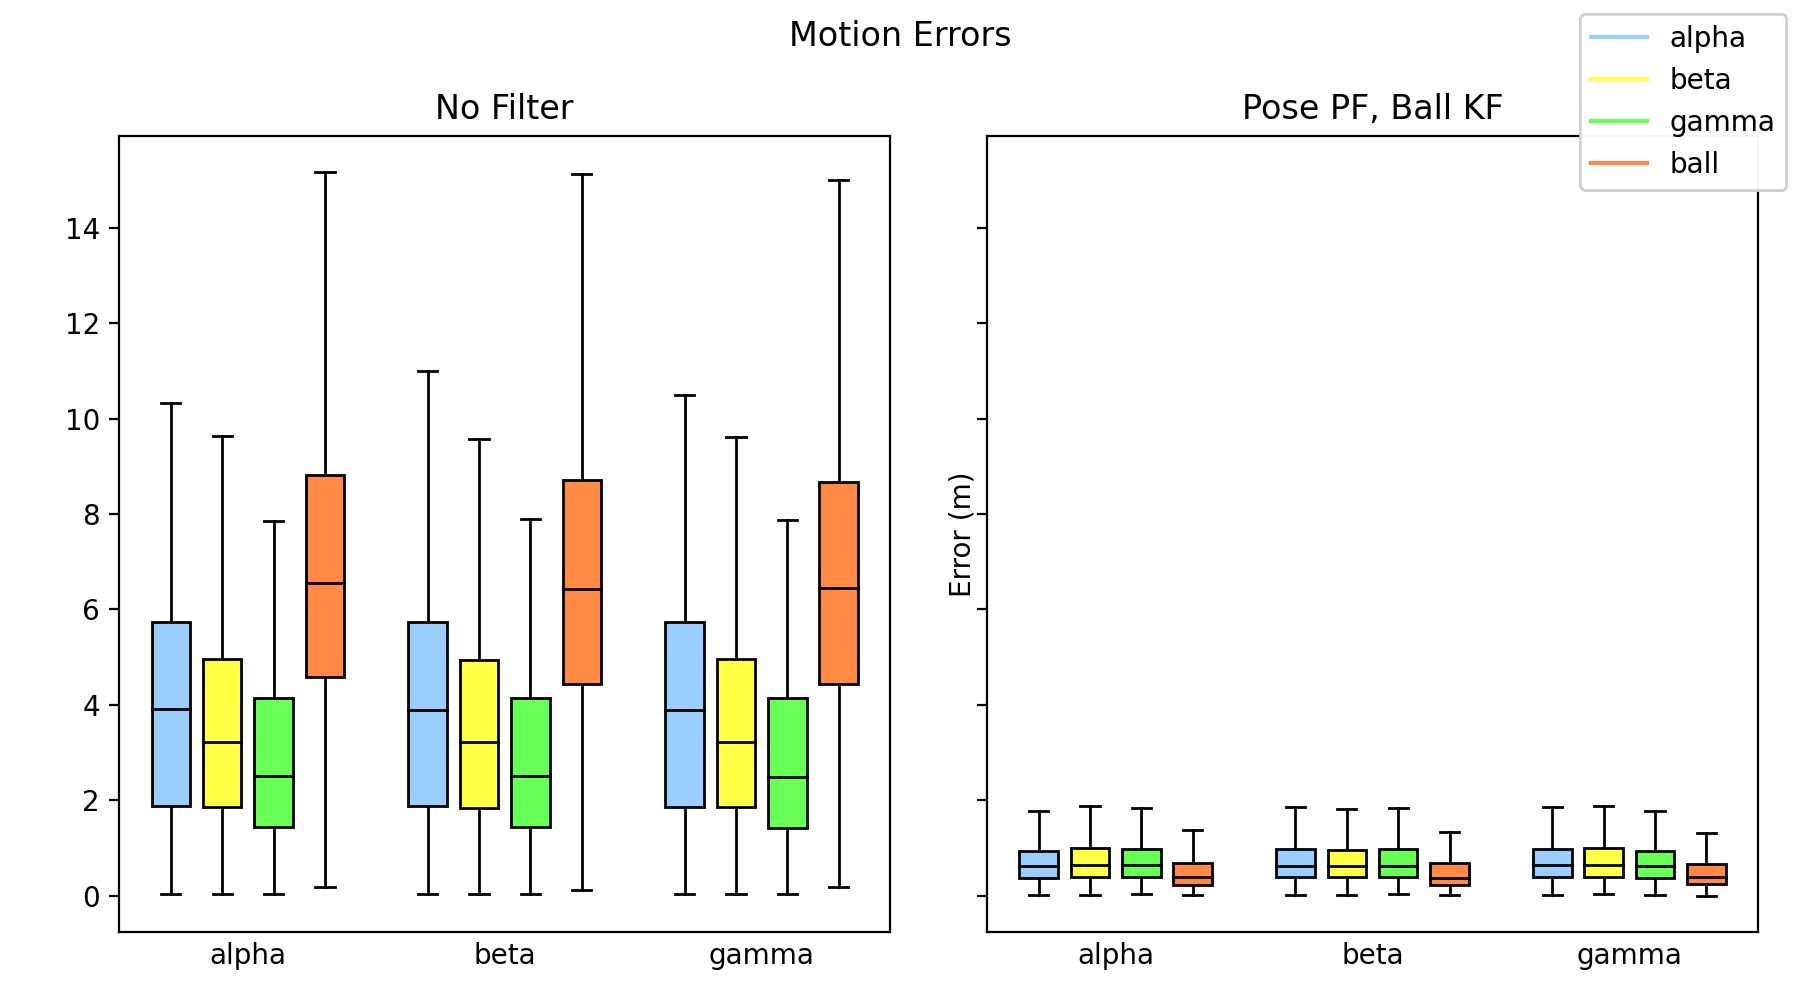
\includegraphics[width=0.9\textwidth]{resources/cfg1_AO_AP_error_motion.png}
    \caption{\textit{Error} \textit{world model} O dan P jaringan baik}
    \label{fig:1-o-p-error}
    \bigskip
\end{figure}

Dari grafik \ref{fig:1-o-p-error} dapat dilihat bahwa ada peningkatan yang sangat signifikan dalam akurasi lokalisasi robot. Dari diagonal lapangan yang sepanjang $10,82$ meter, \textit{world model} O mendapat \textit{error} yang tersebar dalam rentang sebesar itu. Sehingga perbandingan ini menggambarkan seberapa berisiknya \textit{error} sensor yang terakumulasi dalam bacaan odometri seperti sensor lainnya, sedangkan didapatkan bahwa tidak ada perbedaan yang signifikan dari estimasi kecepatan pada penapis partikel berbasis \textit{pose} dan \textit{noise} dari \textit{error} mentah bacaan odometri. Untuk kecepatan bola, karena kecepatan diturunkan dari selisih posisi, masuk akal bahwa estimasi posisi yang lebih baik akan menghasilkan estimasi kecepatan yang lebih baik juga.

\subsection{Perbandingan Algoritma Lokalisasi Penapis Partikel Berbasis \textit{Pose} dan Penapis Partikel Berbasis \textit{Twist}}

Dibandingkan dengan \textit{world model} P, \textit{world model} Q menggunakan penapis partikel berbasis \textit{pose} dan \textit{twist} untuk melakukan lokalisasi, dibanding \textit{pose} saja.

\begin{figure}[p]
    \centering
    \medskip
    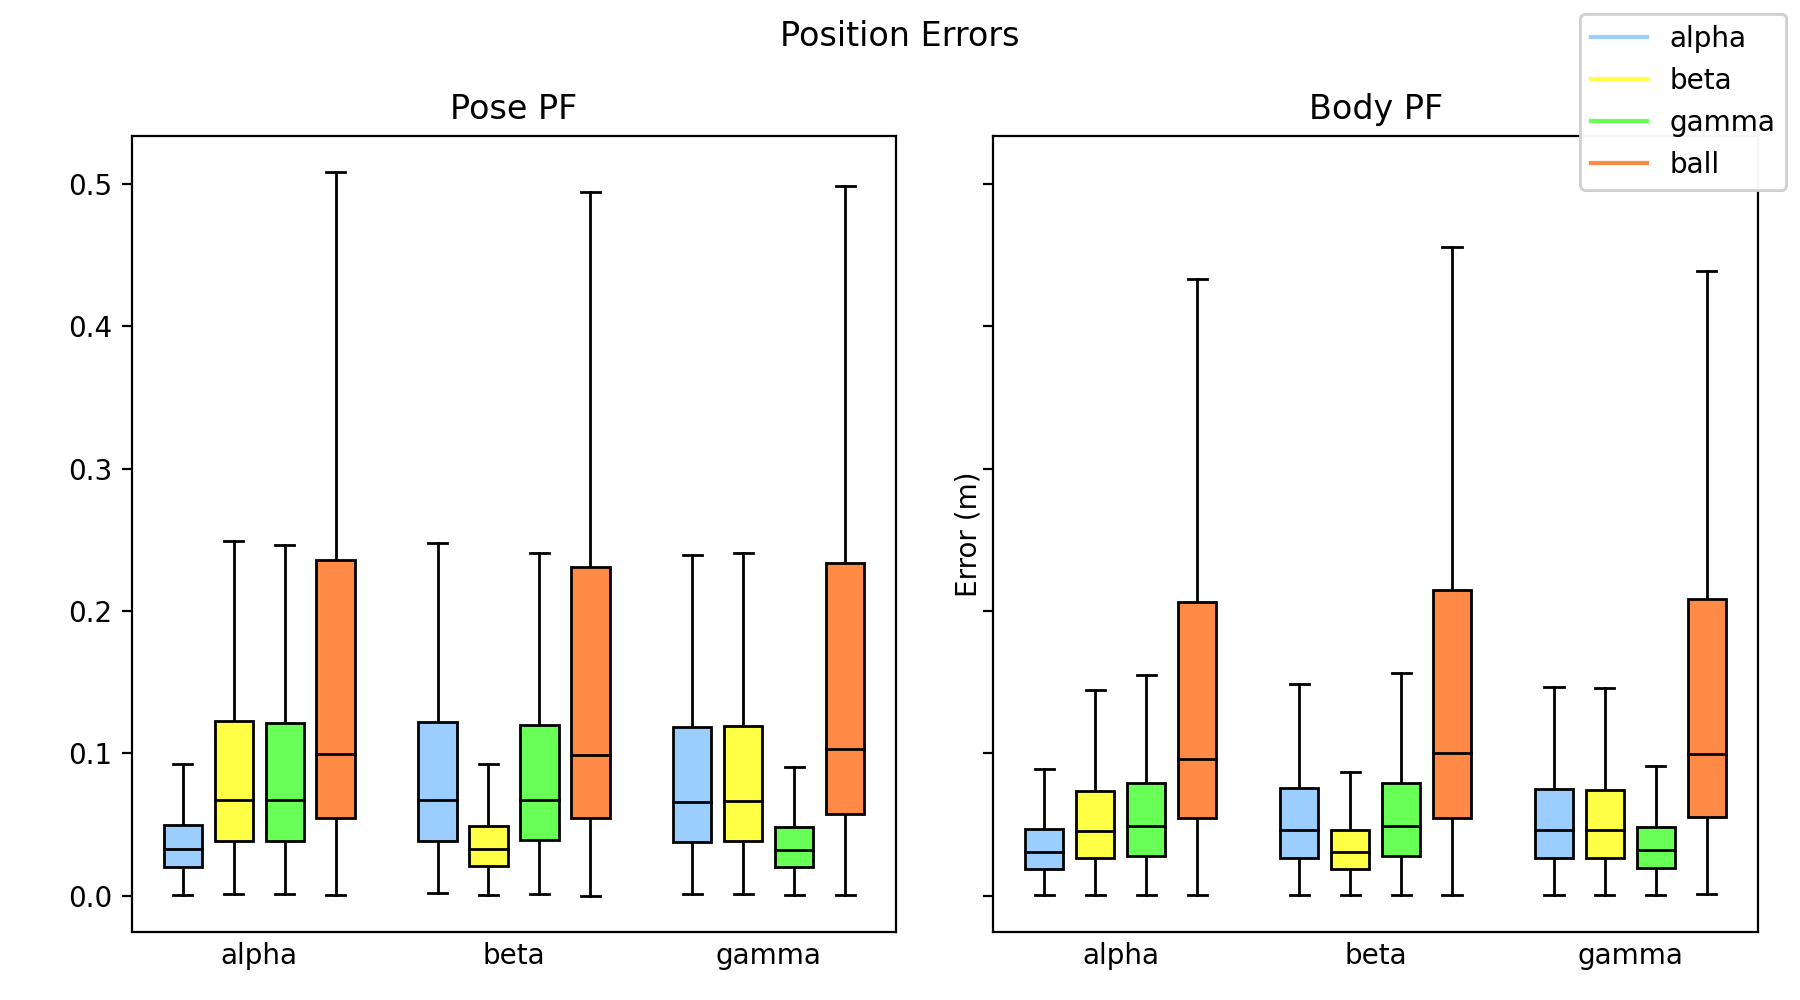
\includegraphics[width=0.9\textwidth]{resources/cfg1_AP_AQ_error_pos.png}
    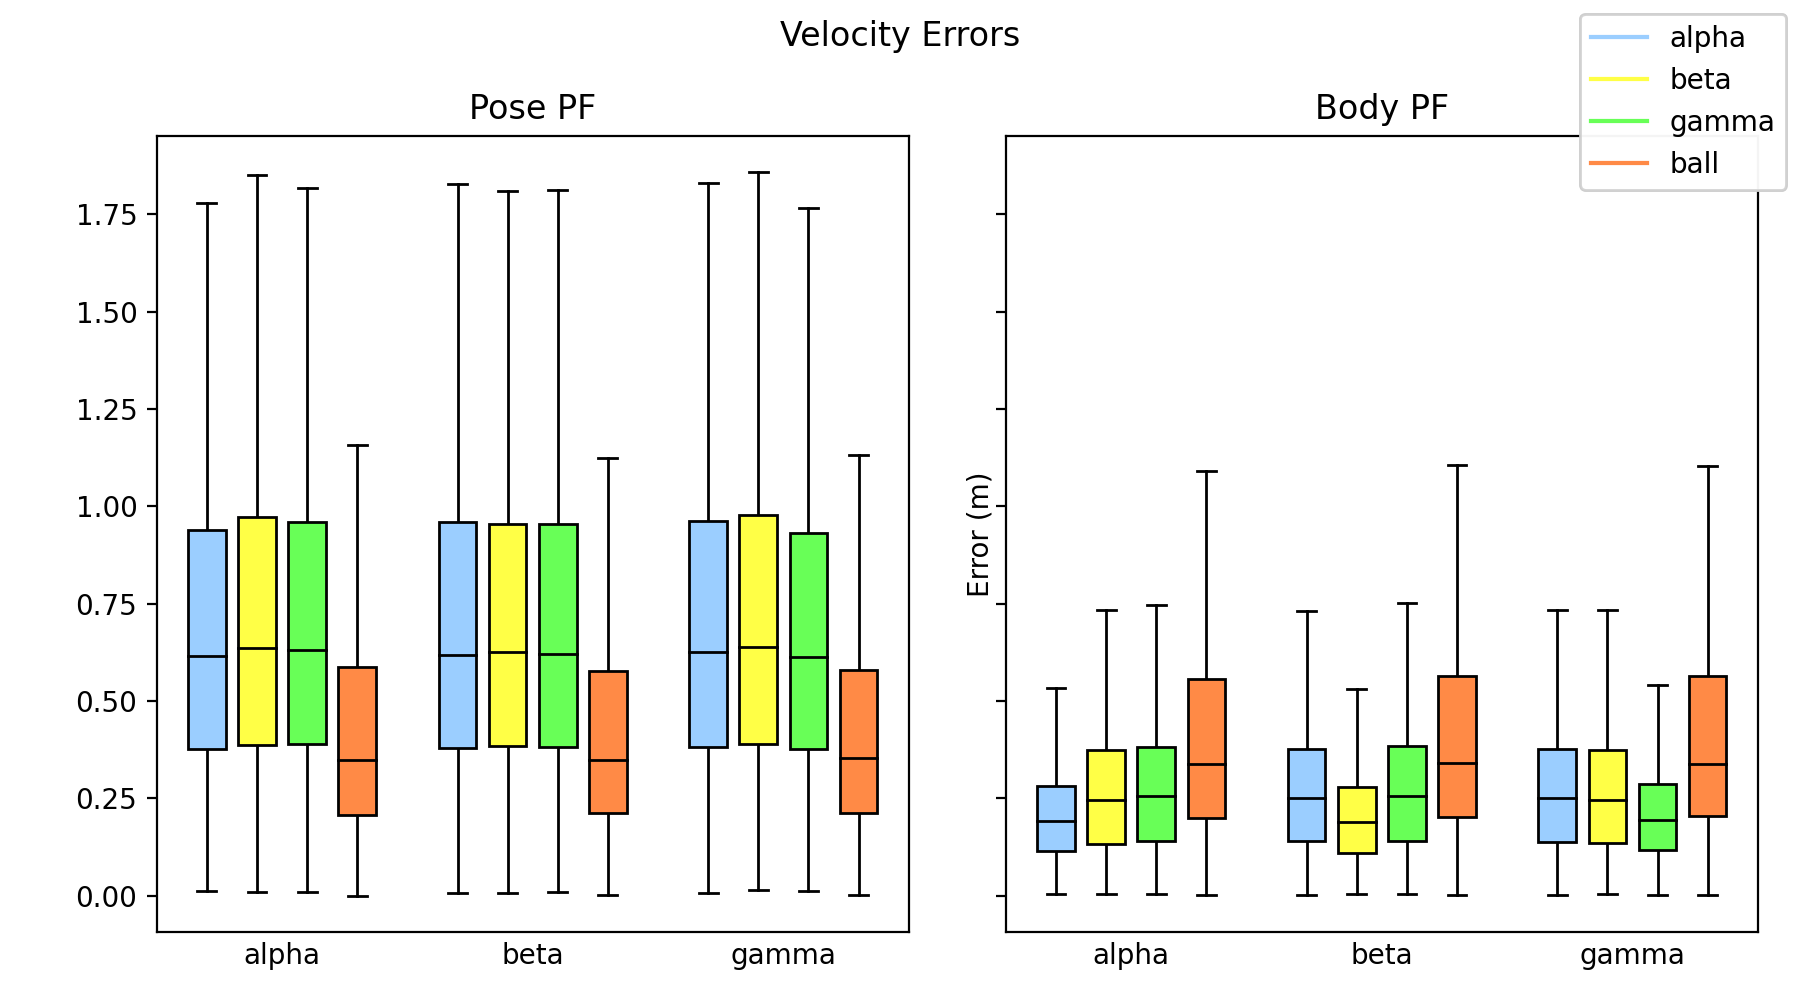
\includegraphics[width=0.9\textwidth]{resources/cfg1_AP_AQ_error_vel.png}
    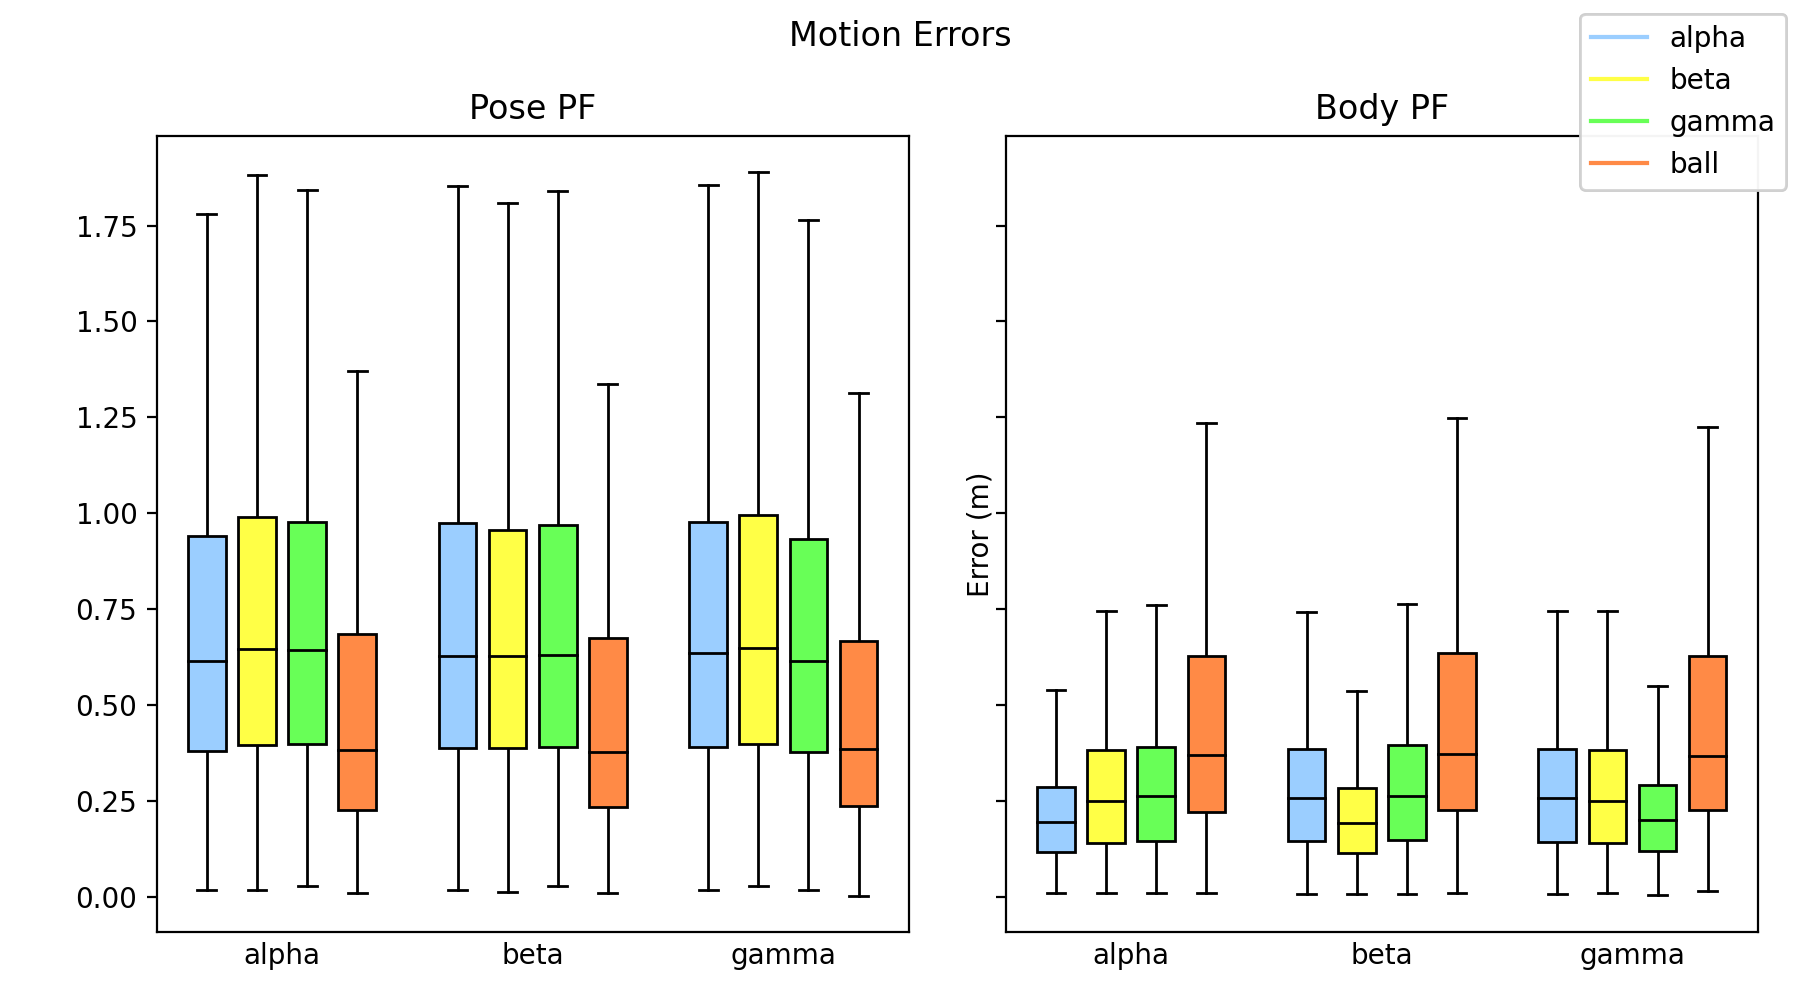
\includegraphics[width=0.9\textwidth]{resources/cfg1_AP_AQ_error_motion.png}
    \caption{\textit{Error} \textit{world model} P dan Q jaringan baik}
    \label{fig:1-p-q-error}
    \bigskip
\end{figure}

Pada grafik \ref{fig:1-p-q-error}, didapatkan bahwa penapis partikel berbasis \textit{pose} dan \textit{twist} dapat memiliki performa yang lebih baik, terutama dalam mengestimasi \textit{twist} dimana median \textit{error} yang didapat sekitar tiga kali lipat lebih baik. Karena penapis partikel berbasis \textit{pose} tidak melacak \textit{twist} dalam partikelnya mengakibatkan penapis tidak mengetahui pergerakan jangka panjang dari robot dan hanya memaksimalkan informasi persepsi \textit{landmark} dan kompasnya saja, sehingga tidak dapat seakurat penapis berbasis \textit{pose} dan \textit{twist}. Perhatikan juga dari grafik posisi bahwa peningkatan akurasi dari lokalisasi dapat meningkatkan akurasi dari estimasi gerakan bola, walaupun sedikit, karena estimasi bola bergantung pada hasil lokalisasi.

\subsection{Perbandingan Algoritma Estimasi Bola Menggunakan Penapis Kalman dan Penapis Partikel}

Dibandingkan dengan \textit{world model} Q, \textit{world model} R menggunakan penapis partikel untuk mengestimasi gerakan dari bola, daripada menggunakan penapis Kalman.

\begin{figure}[p]
    \centering
    \medskip
    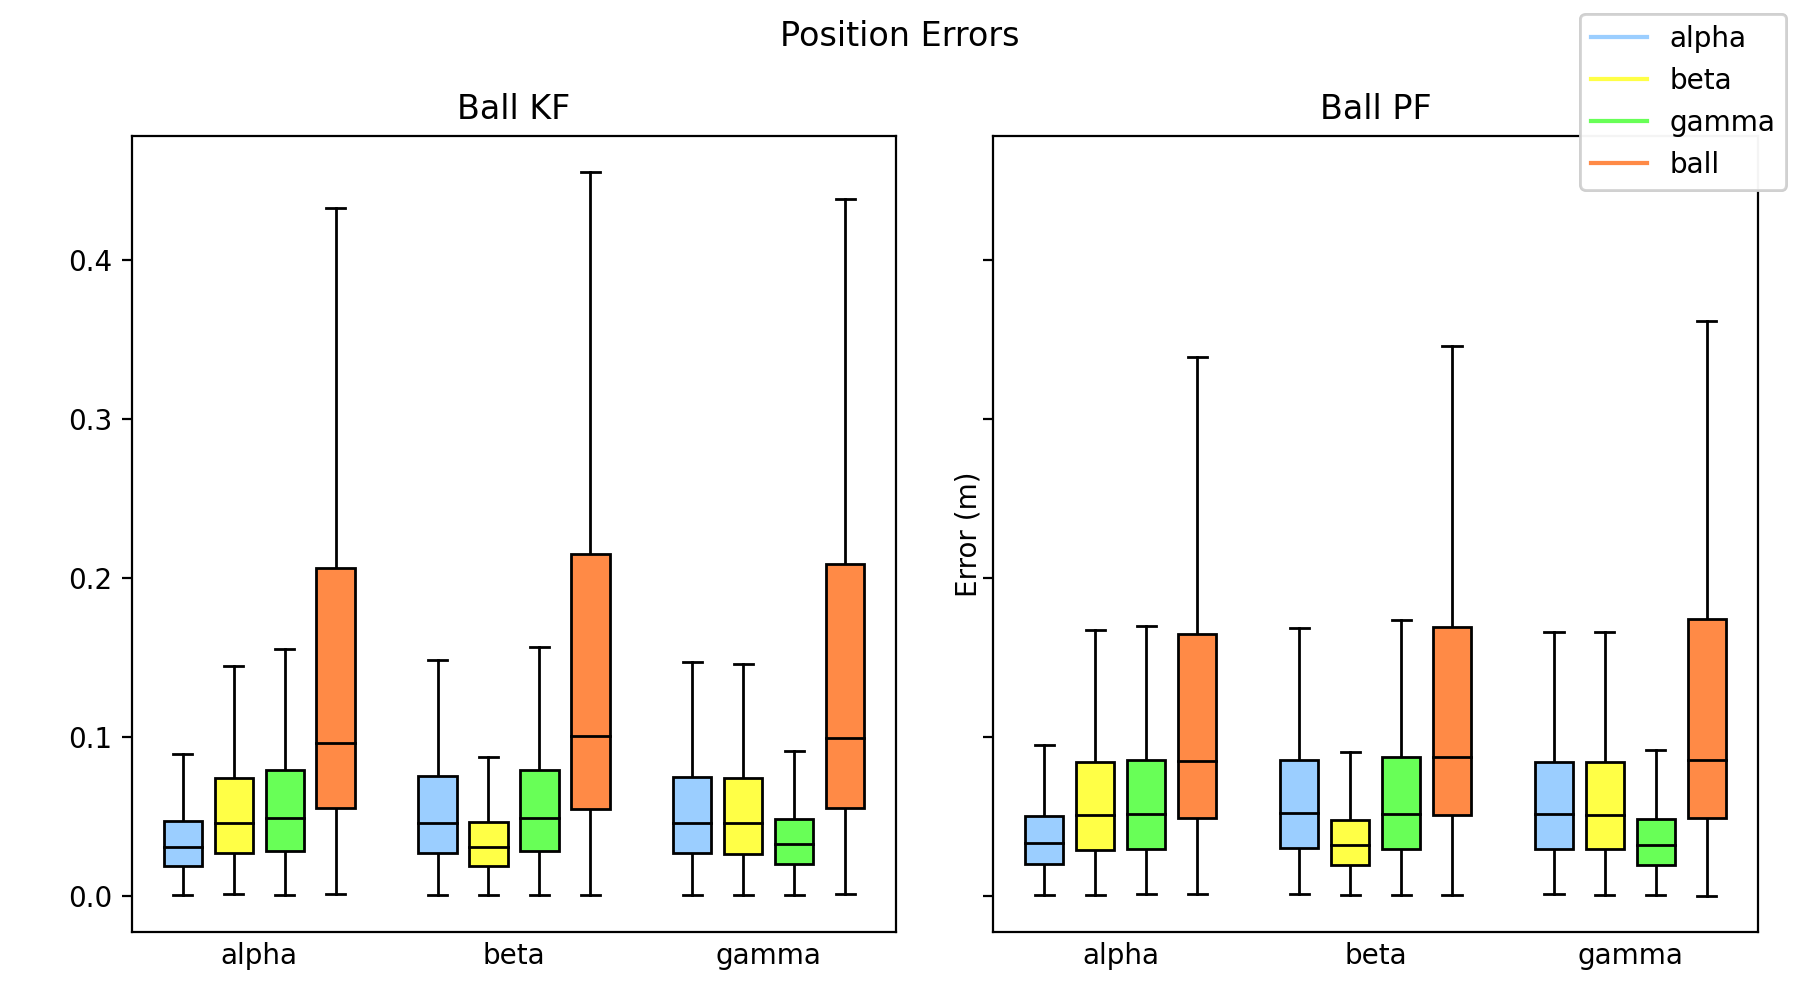
\includegraphics[width=0.9\textwidth]{resources/cfg1_AQ_AR_error_pos.png}
    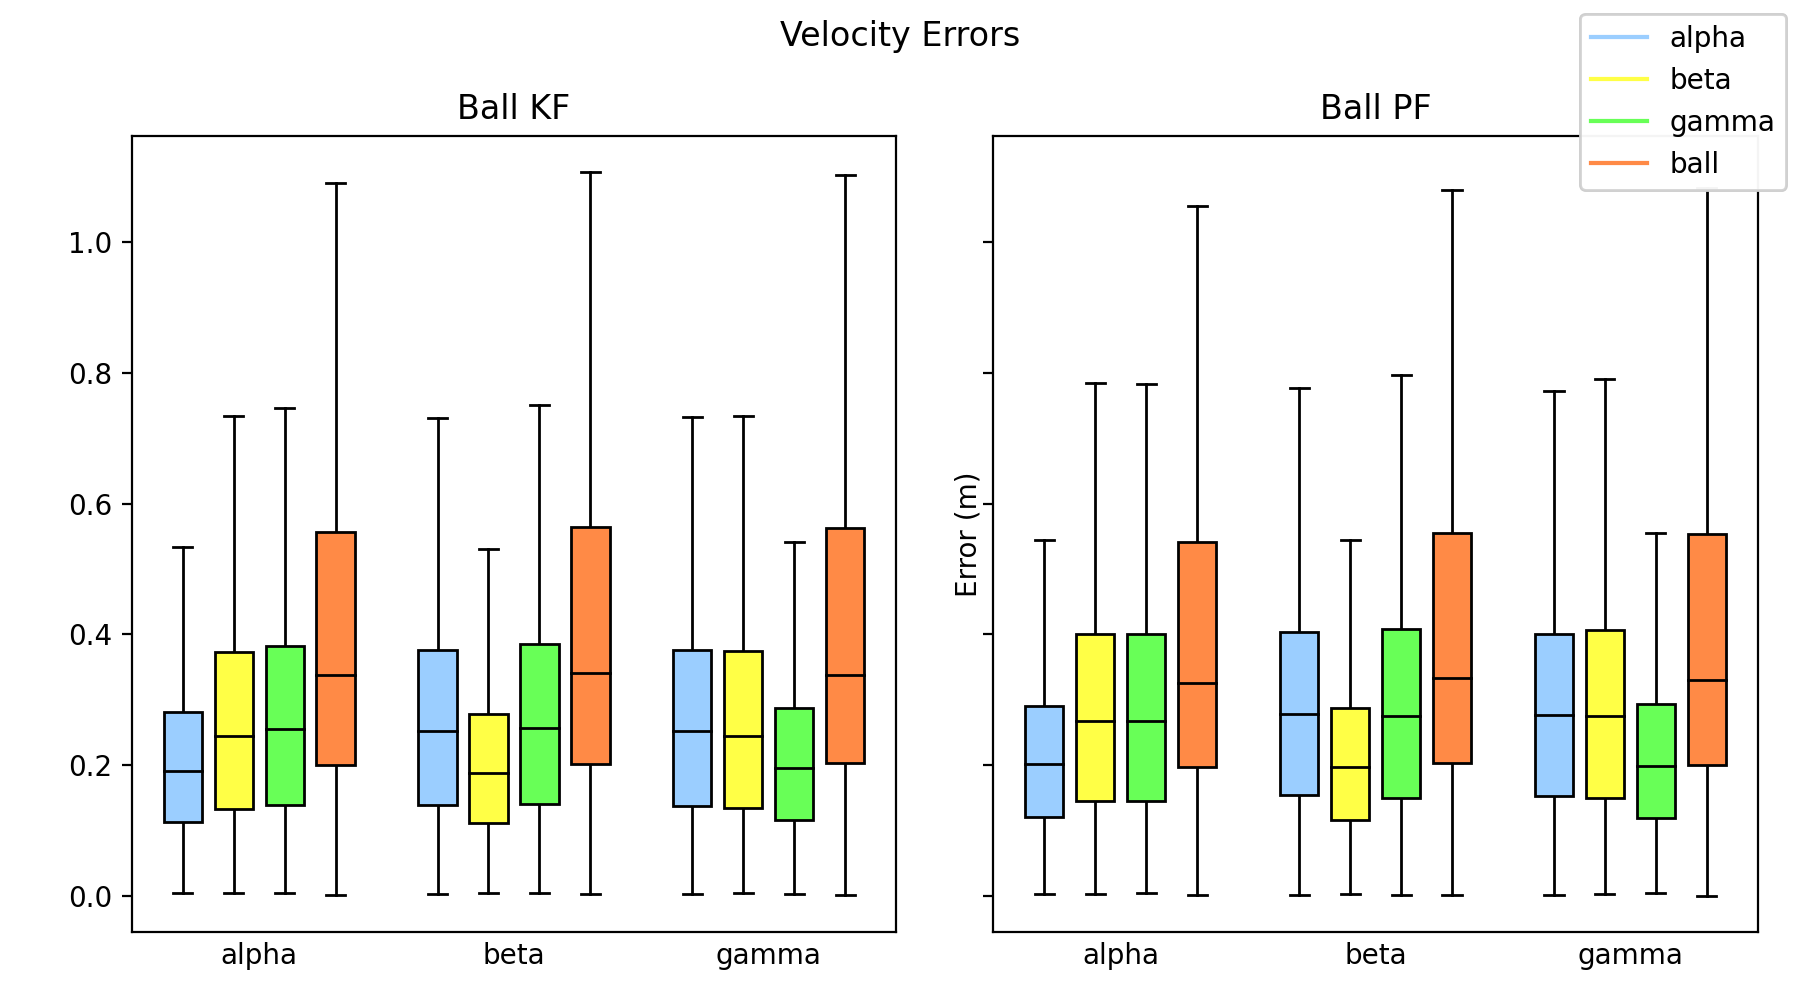
\includegraphics[width=0.9\textwidth]{resources/cfg1_AQ_AR_error_vel.png}
    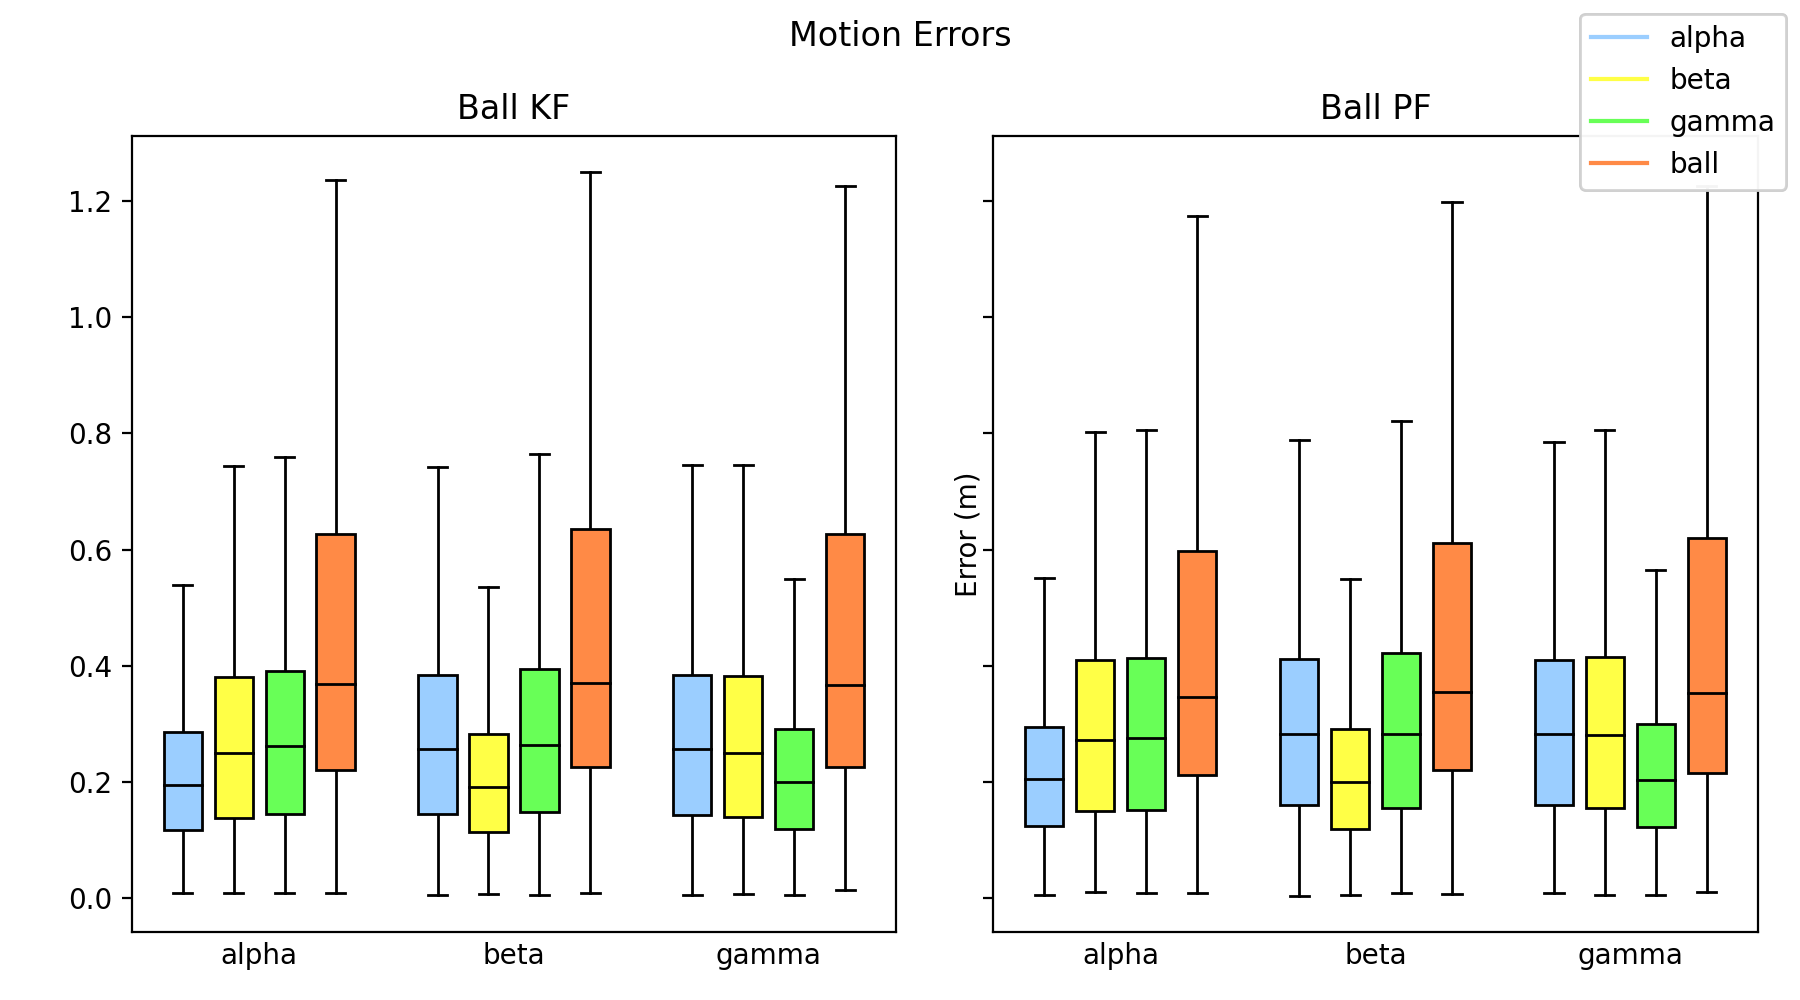
\includegraphics[width=0.9\textwidth]{resources/cfg1_AQ_AR_error_motion.png}
    \caption{\textit{Error} \textit{world model} Q dan R jaringan baik}
    \label{fig:1-q-r-error}
    \bigskip
\end{figure}

Pada grafik \ref{fig:1-q-r-error}, terdapat peningkatan kecil dalam penggunaan penapis partikel dibanding dengan menggunakan penapis Kalman. Hal ini tampaknya disebabkan karena pemodelan pengukuran pada penapis Kalman yang tidak eksak sama dengan profil \textit{error} dari \textit{vision} yang membedakan \textit{error} sejajar dan tegak lurus dengan besar tergantung dari jarak objek, jika dibandingkan dengan penapis partikel yang dapat dengan eksak memodelkan profil \textit{error} tersebut.

\subsection{Perbandingan Algoritma dengan Penyesuaian Waktu dan tanpa Penyesuaian Waktu}

Dibandingkan dengan \textit{world model} R, \textit{world model} RB dibuat tanpa melakukan penyesuaian waktu antara \textit{timestamp} data estimasi dan waktu sekarang saat mengirimkan hasil estimasi ke evaluator.

\begin{figure}[p]
    \centering
    \medskip
    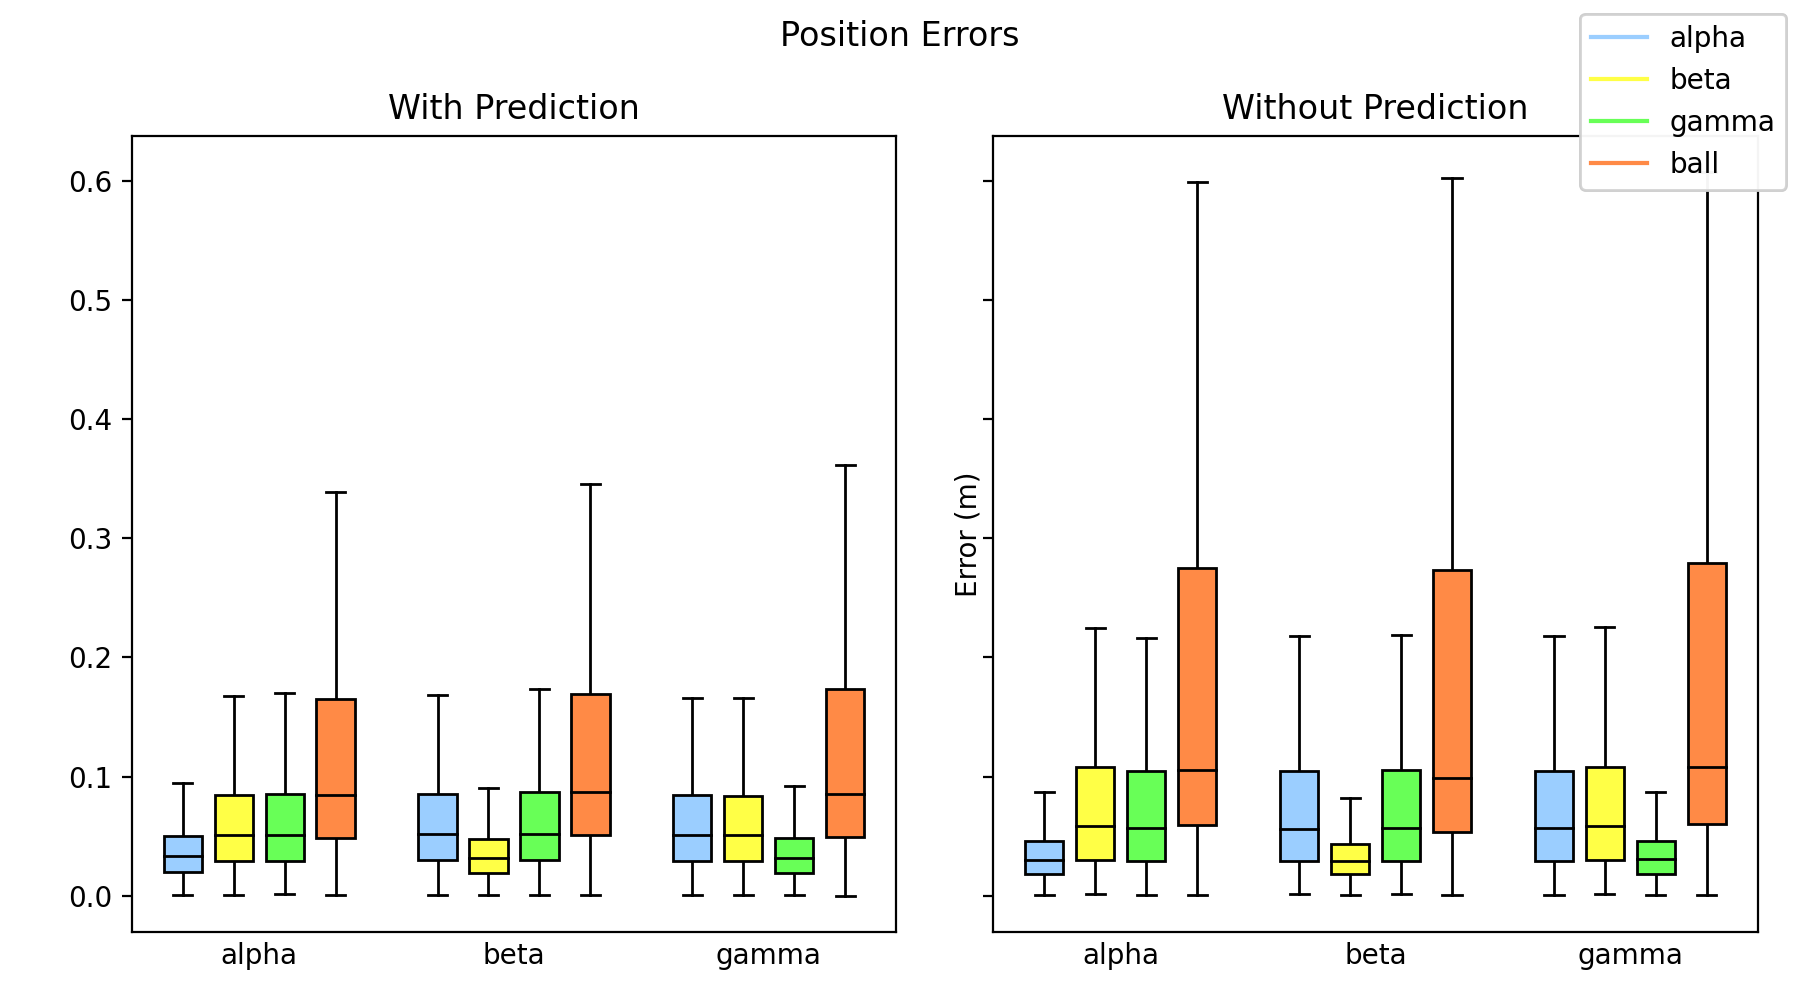
\includegraphics[width=0.9\textwidth]{resources/cfg1_AR_ARB_error_pos.png}
    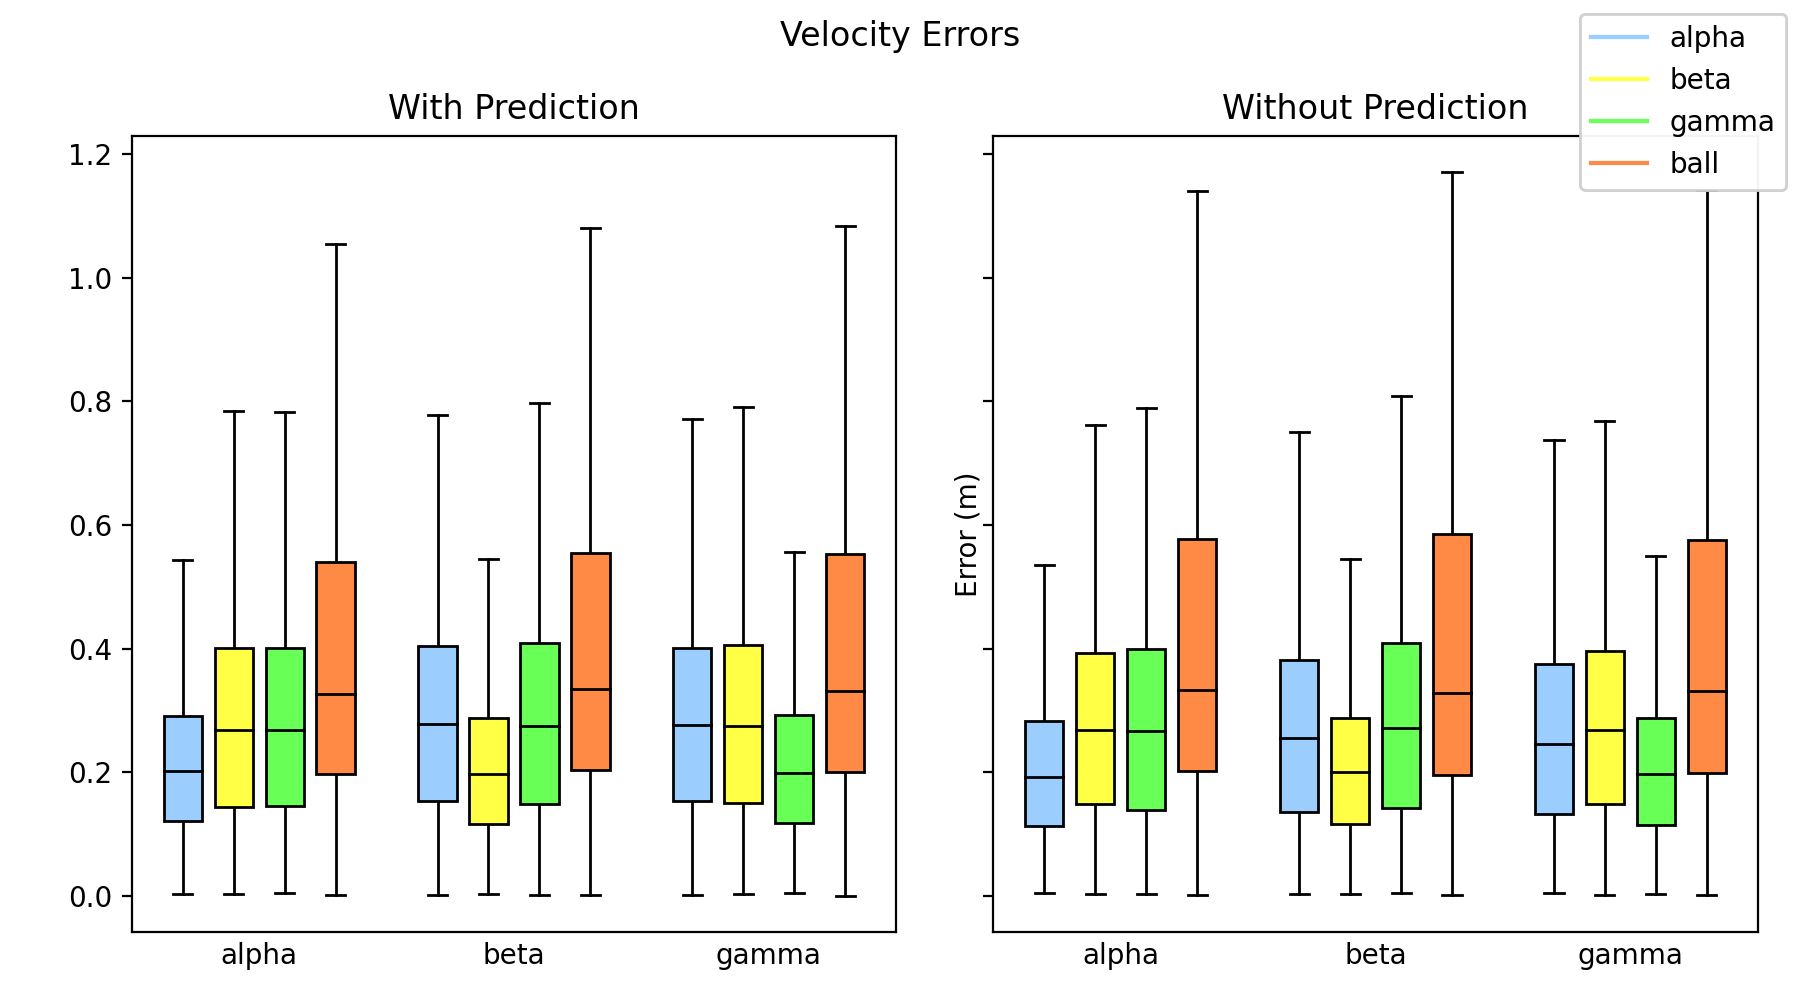
\includegraphics[width=0.9\textwidth]{resources/cfg1_AR_ARB_error_vel.png}
    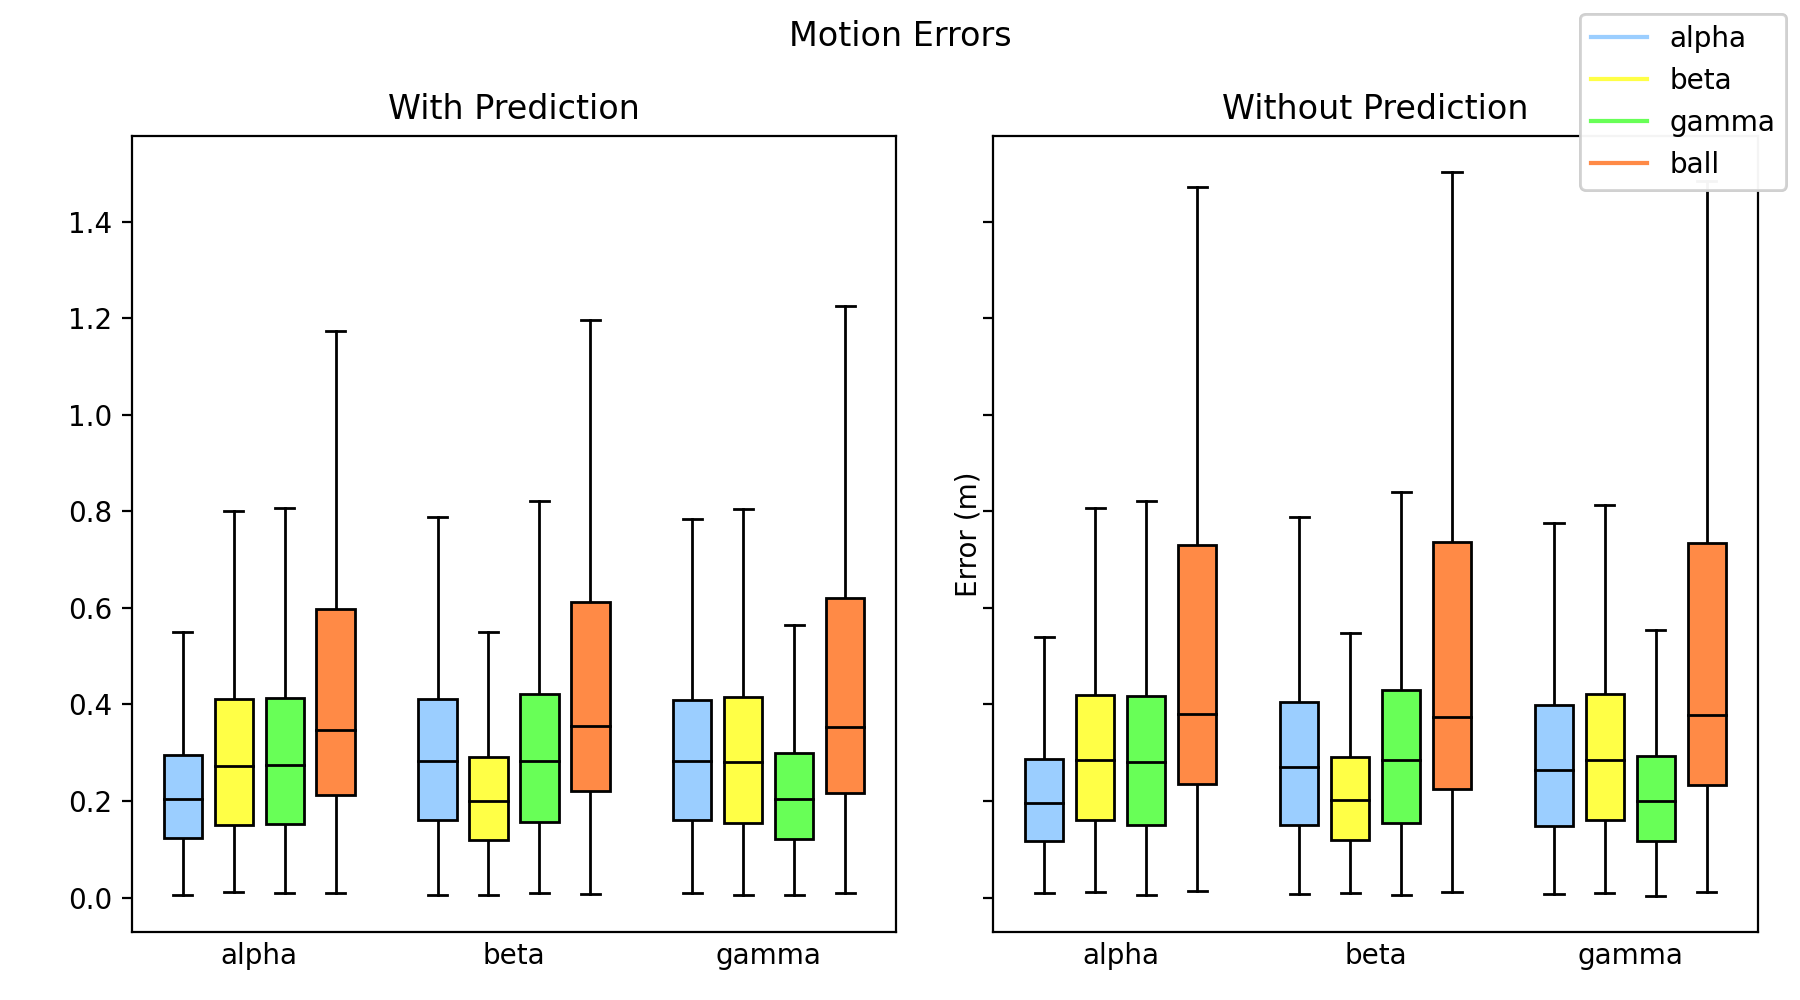
\includegraphics[width=0.9\textwidth]{resources/cfg1_AR_ARB_error_motion.png}
    \caption{\textit{Error} \textit{world model} R dan RB jaringan baik}
    \label{fig:1-r-rb-error}
    \bigskip
\end{figure}

Pada grafik \ref{fig:1-r-rb-error}, hasil estimasi posisi yang tidak dikompensasi cukup lebih buruk jika dibandingkan dengan estimasi dengan kompensasi waktu. Maka dapat dilihat kompensasi waktu dapat membantu untuk meningkatkan akurasi estimasi untuk objek seperti robot teman yang mungkin terlambat karena latensi atau bola yang mungkin tidak dipersepsi atau datanya terlambat karena latensi.

\section{Pengujian dan Analisis Algoritma Estimasi Data Terlambat}

\subsection{Perbandingan Algoritma Estimasi Bola Menggunakan PF dan OOSM-PF}

Dibandingkan dengan \textit{world model} R, \textit{world model} S menggunakan modifikasi OOSM-PF untuk dapat mengintegrasi data bola teman yang terlambat, daripada dengan PF biasa.

\begin{figure}[p]
    \centering
    \medskip
    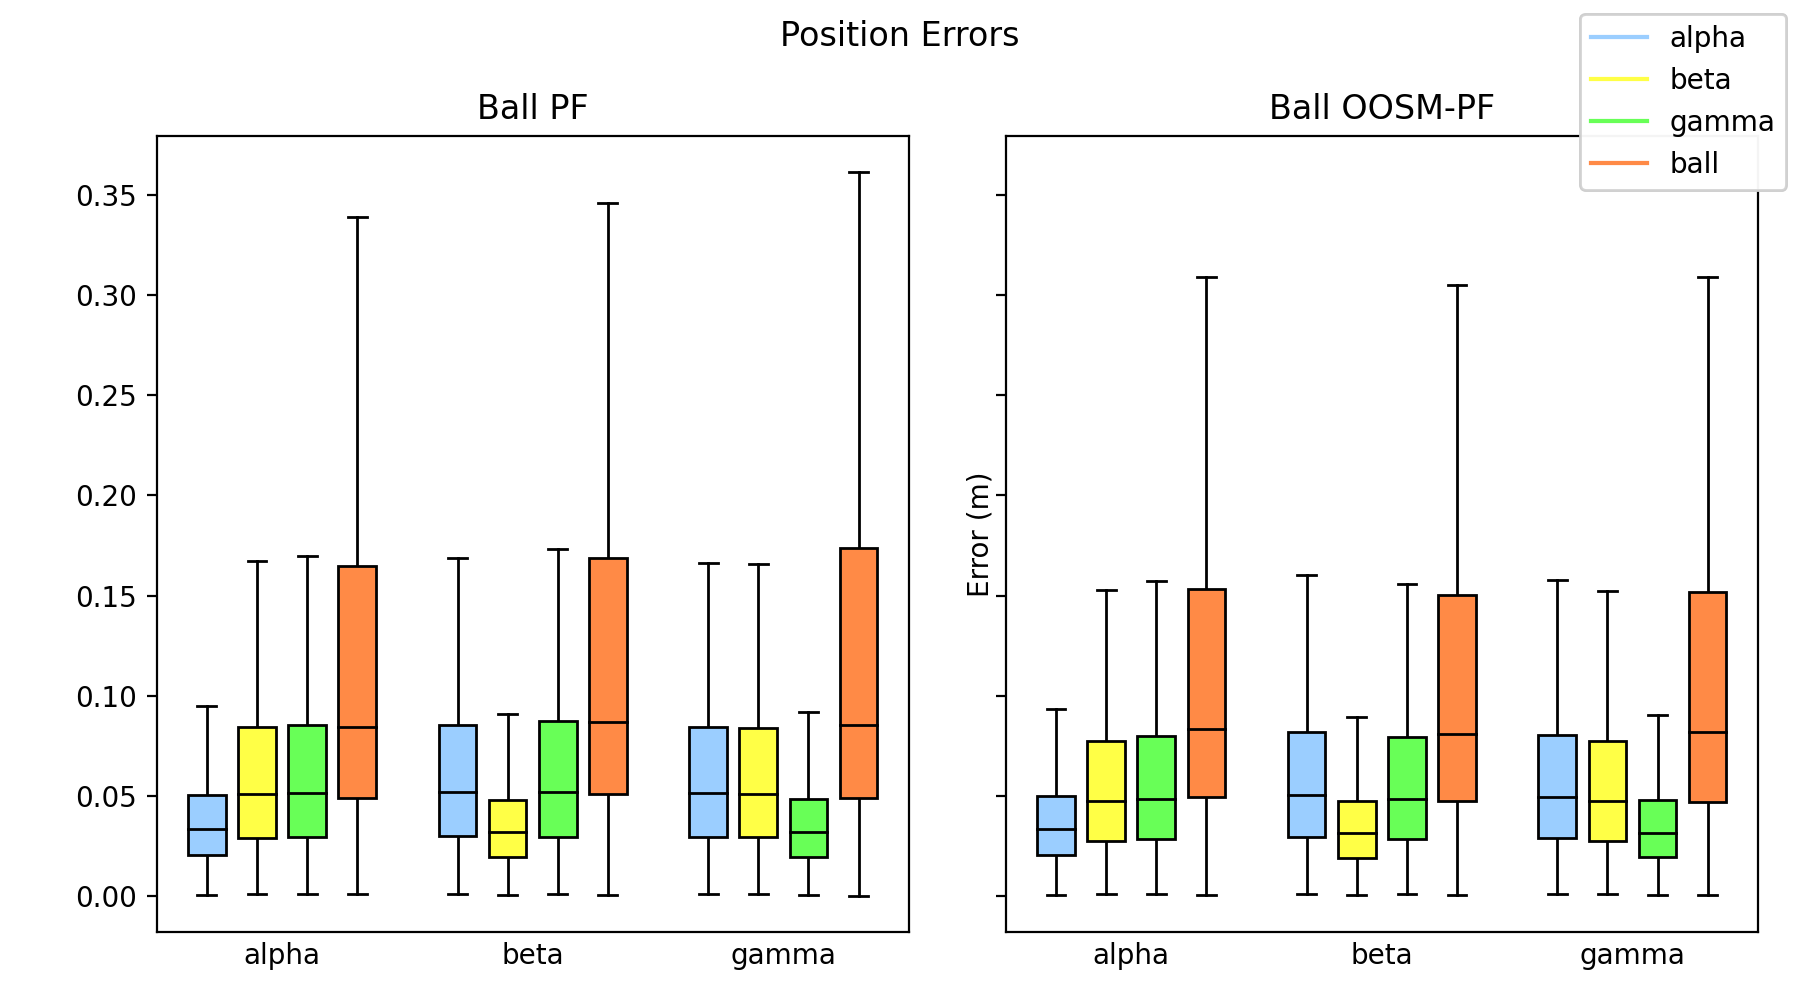
\includegraphics[width=0.9\textwidth]{resources/cfg1_AR_AS_error_pos.png}
    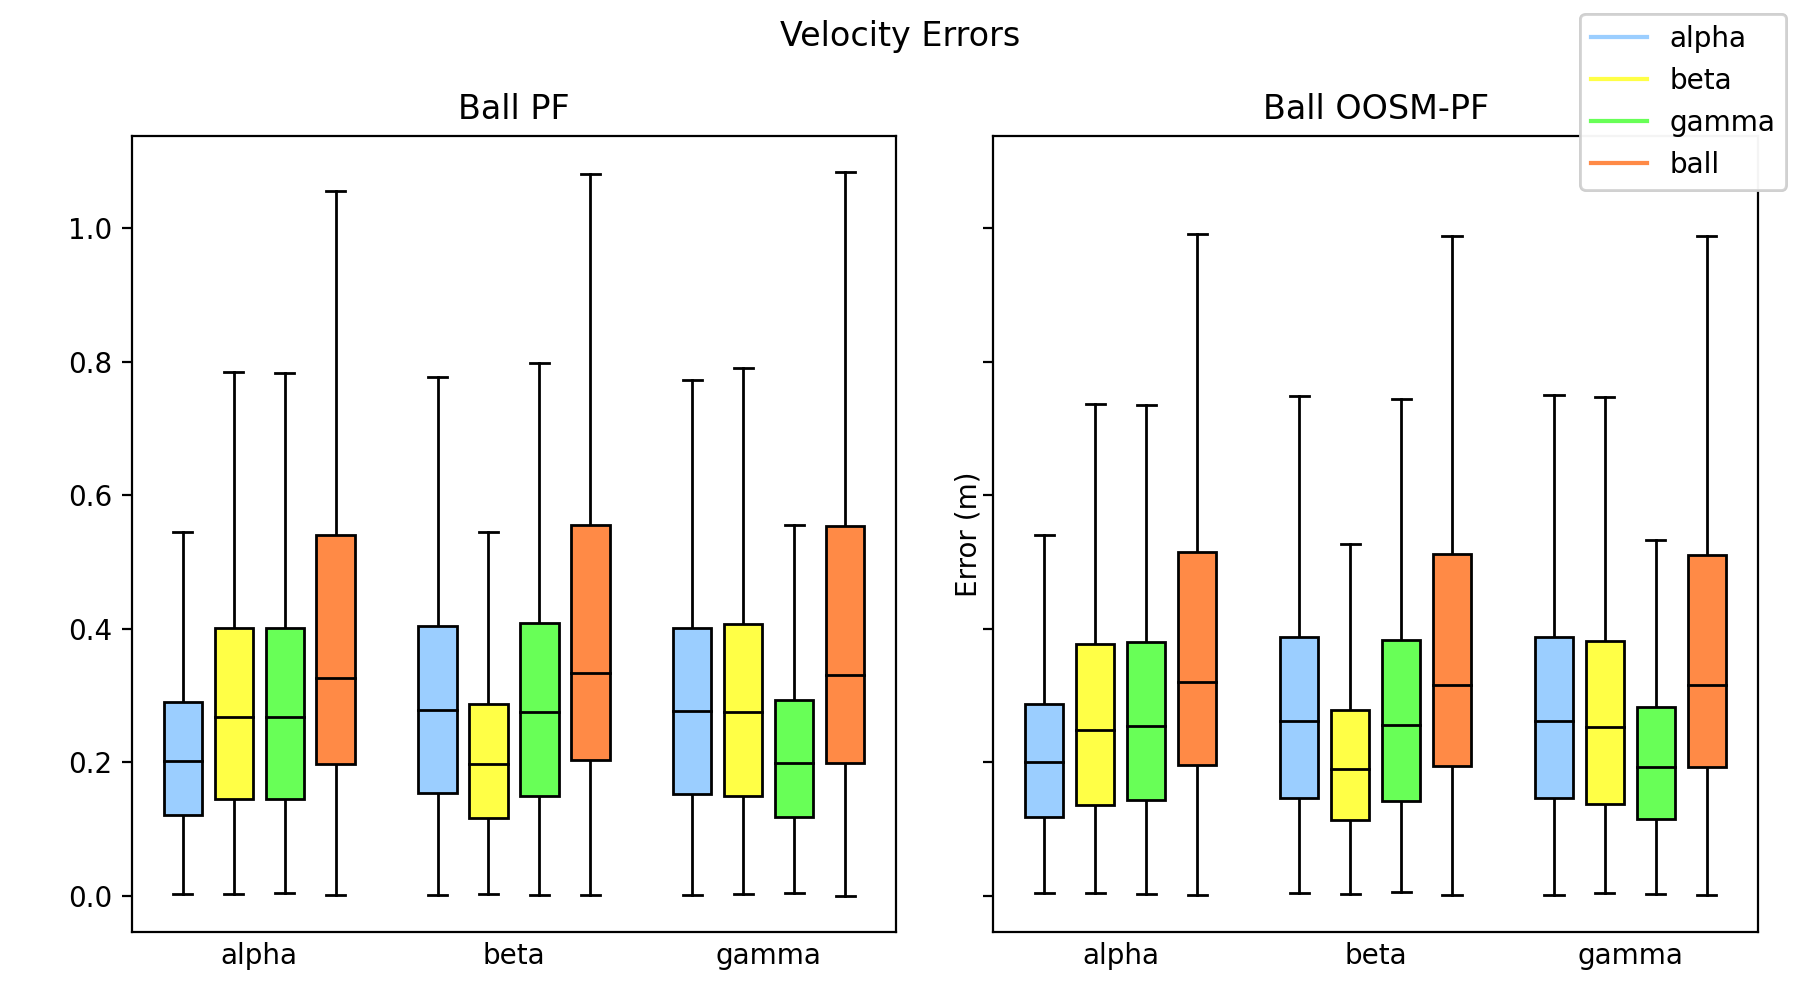
\includegraphics[width=0.9\textwidth]{resources/cfg1_AR_AS_error_vel.png}
    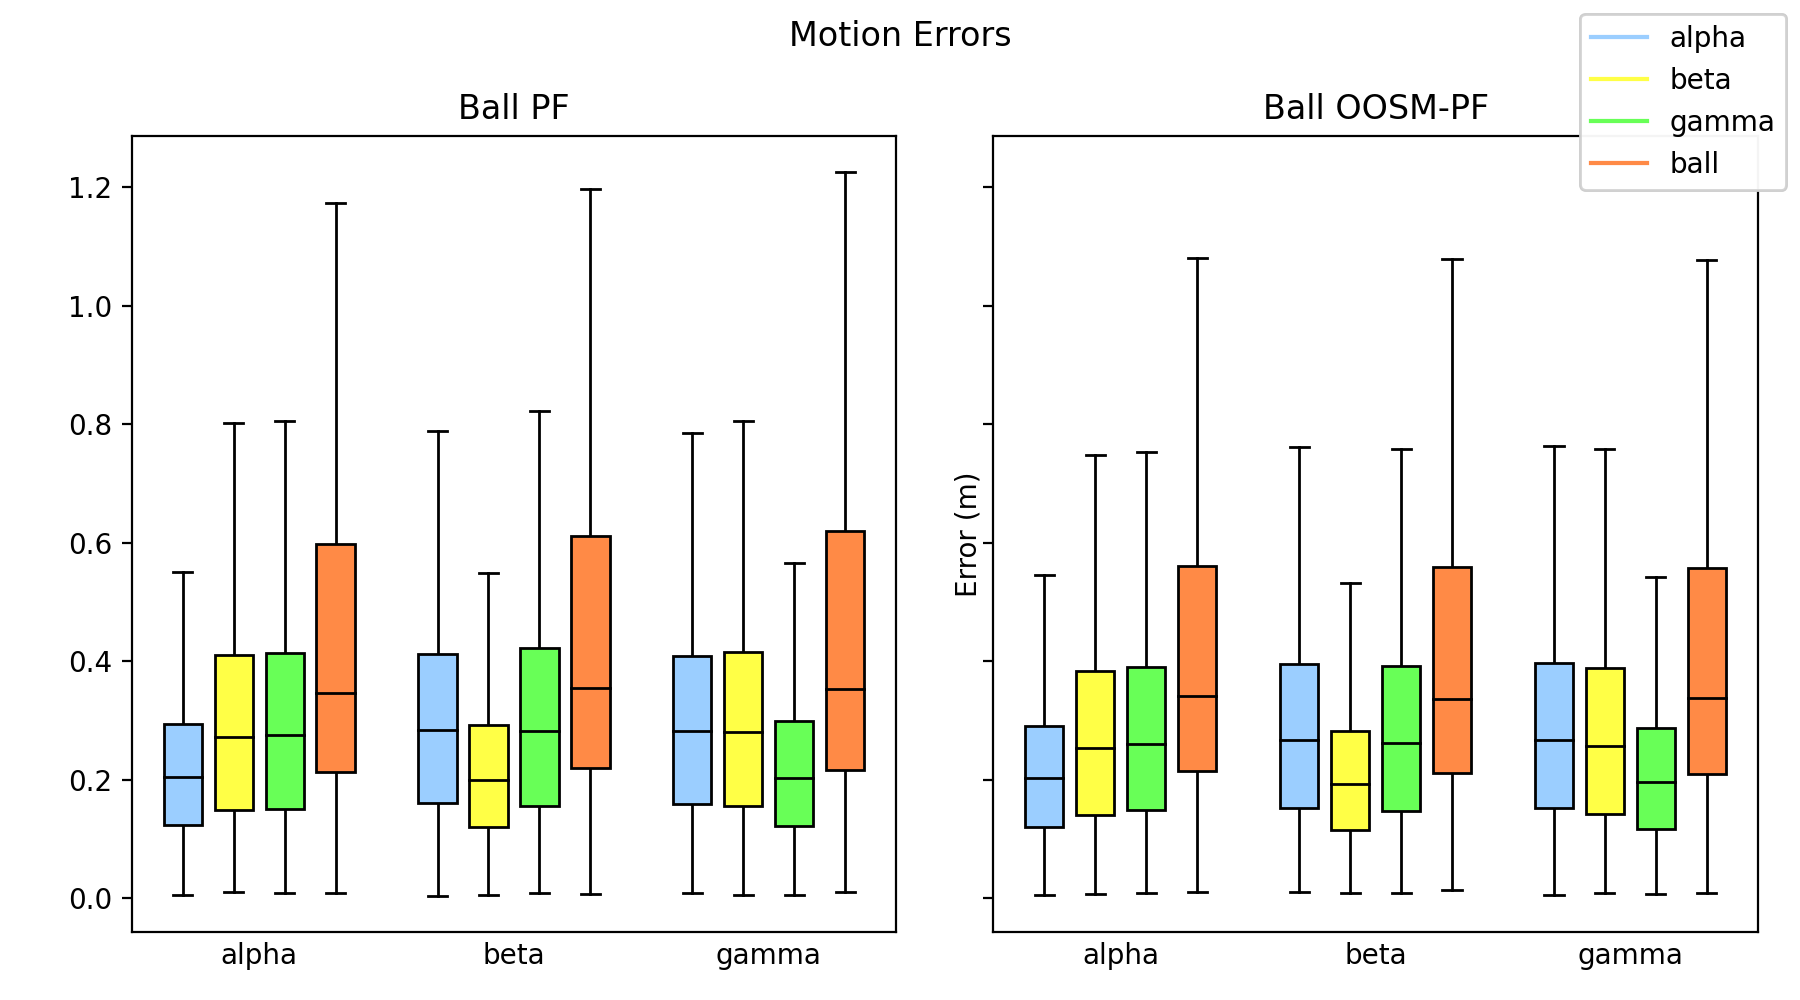
\includegraphics[width=0.9\textwidth]{resources/cfg1_AR_AS_error_motion.png}
    \caption{\textit{Error} \textit{world model} R dan S jaringan baik}
    \label{fig:1-r-s-error}
    \bigskip
\end{figure}

\begin{figure}[p]
    \centering
    \medskip
    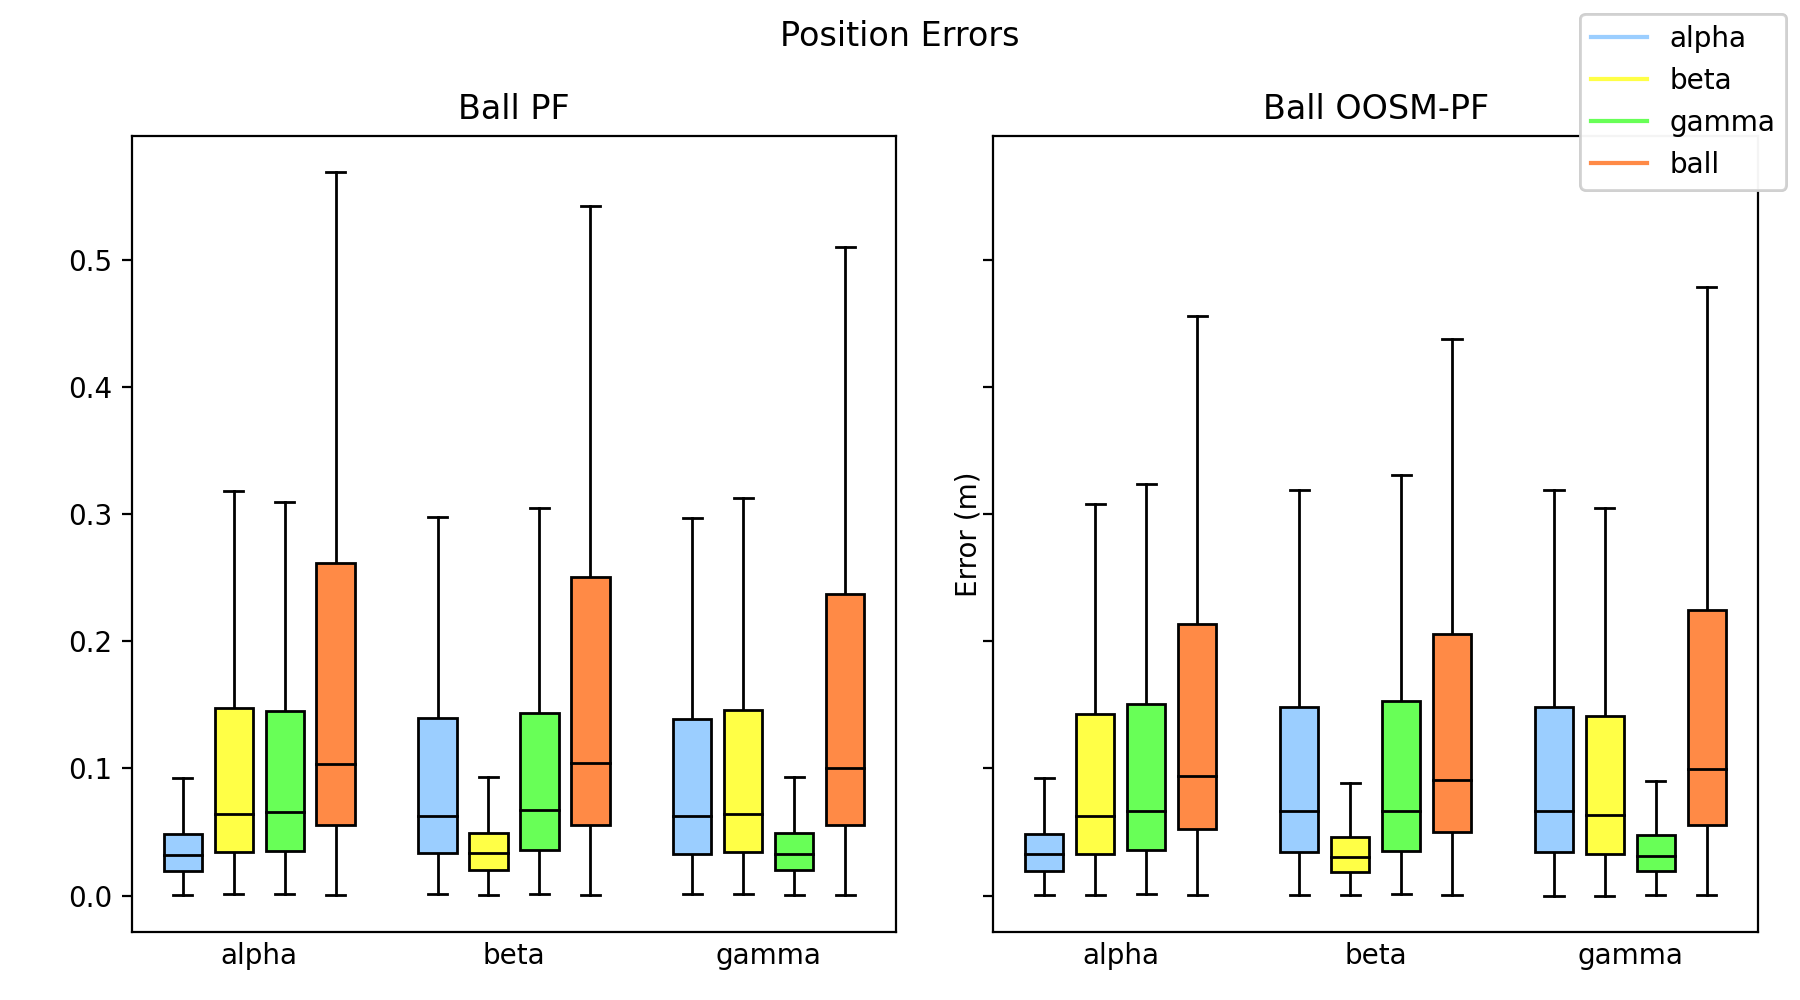
\includegraphics[width=0.9\textwidth]{resources/cfg2_AR_AS_error_pos.png}
    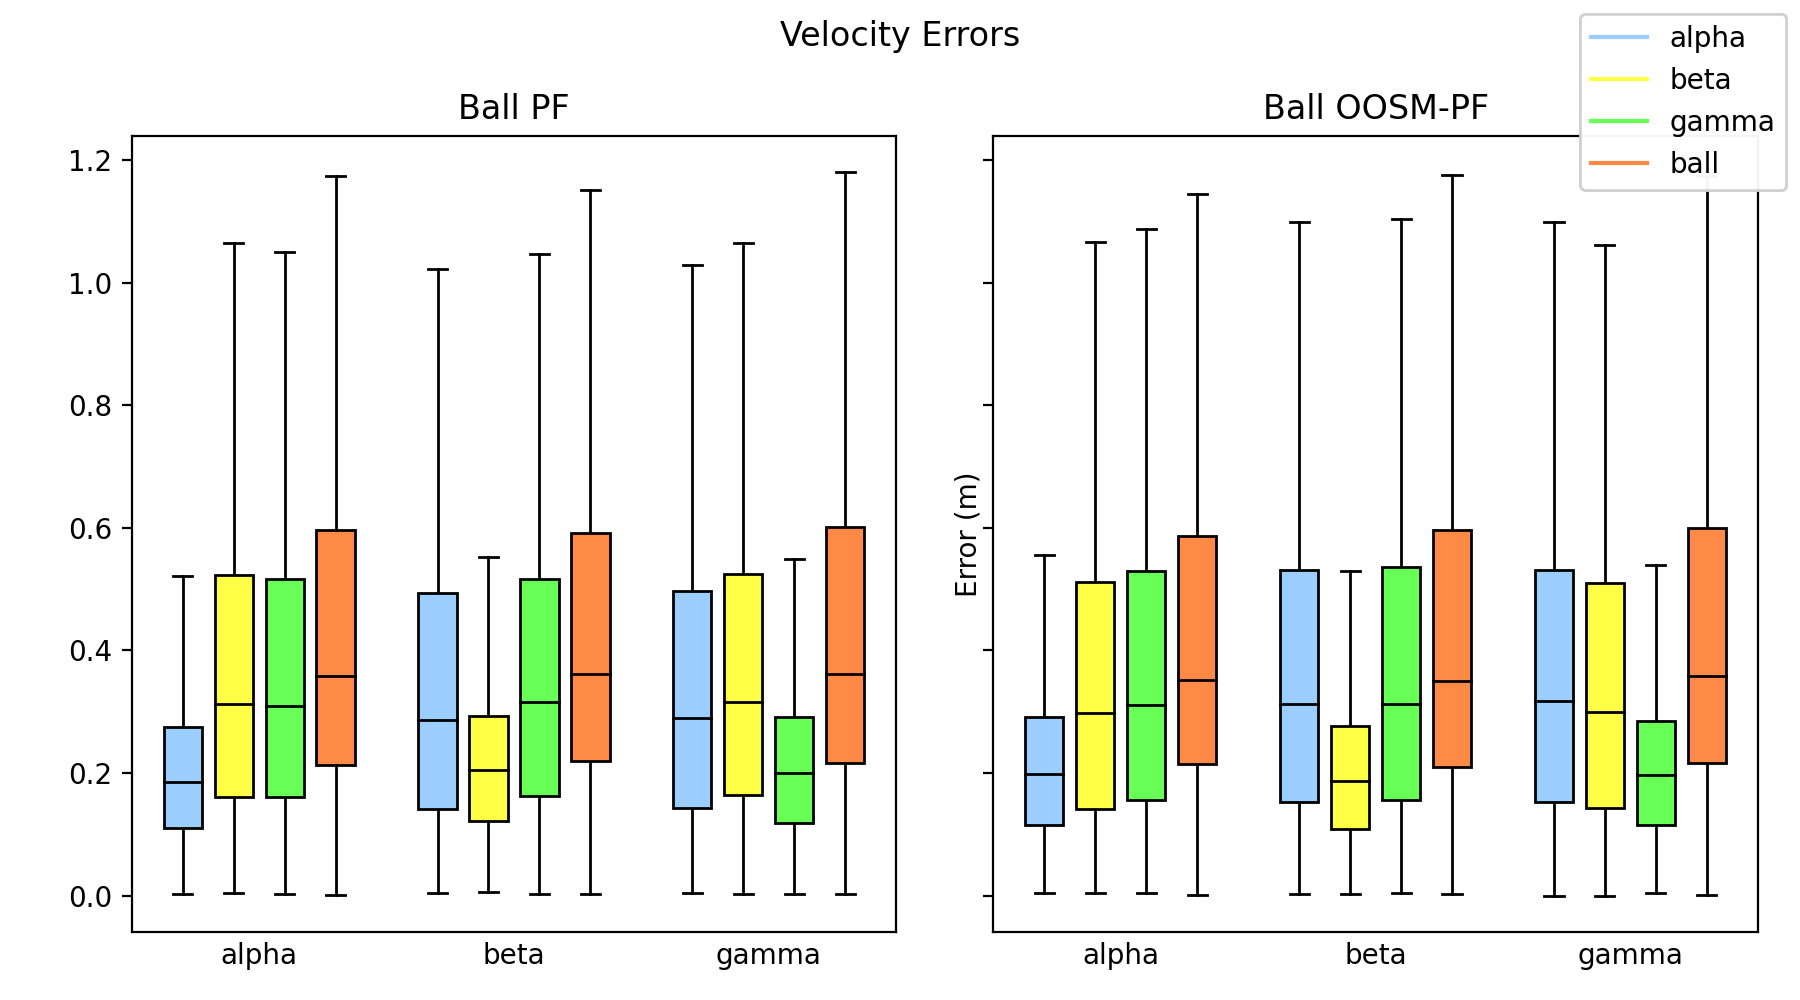
\includegraphics[width=0.9\textwidth]{resources/cfg2_AR_AS_error_vel.png}
    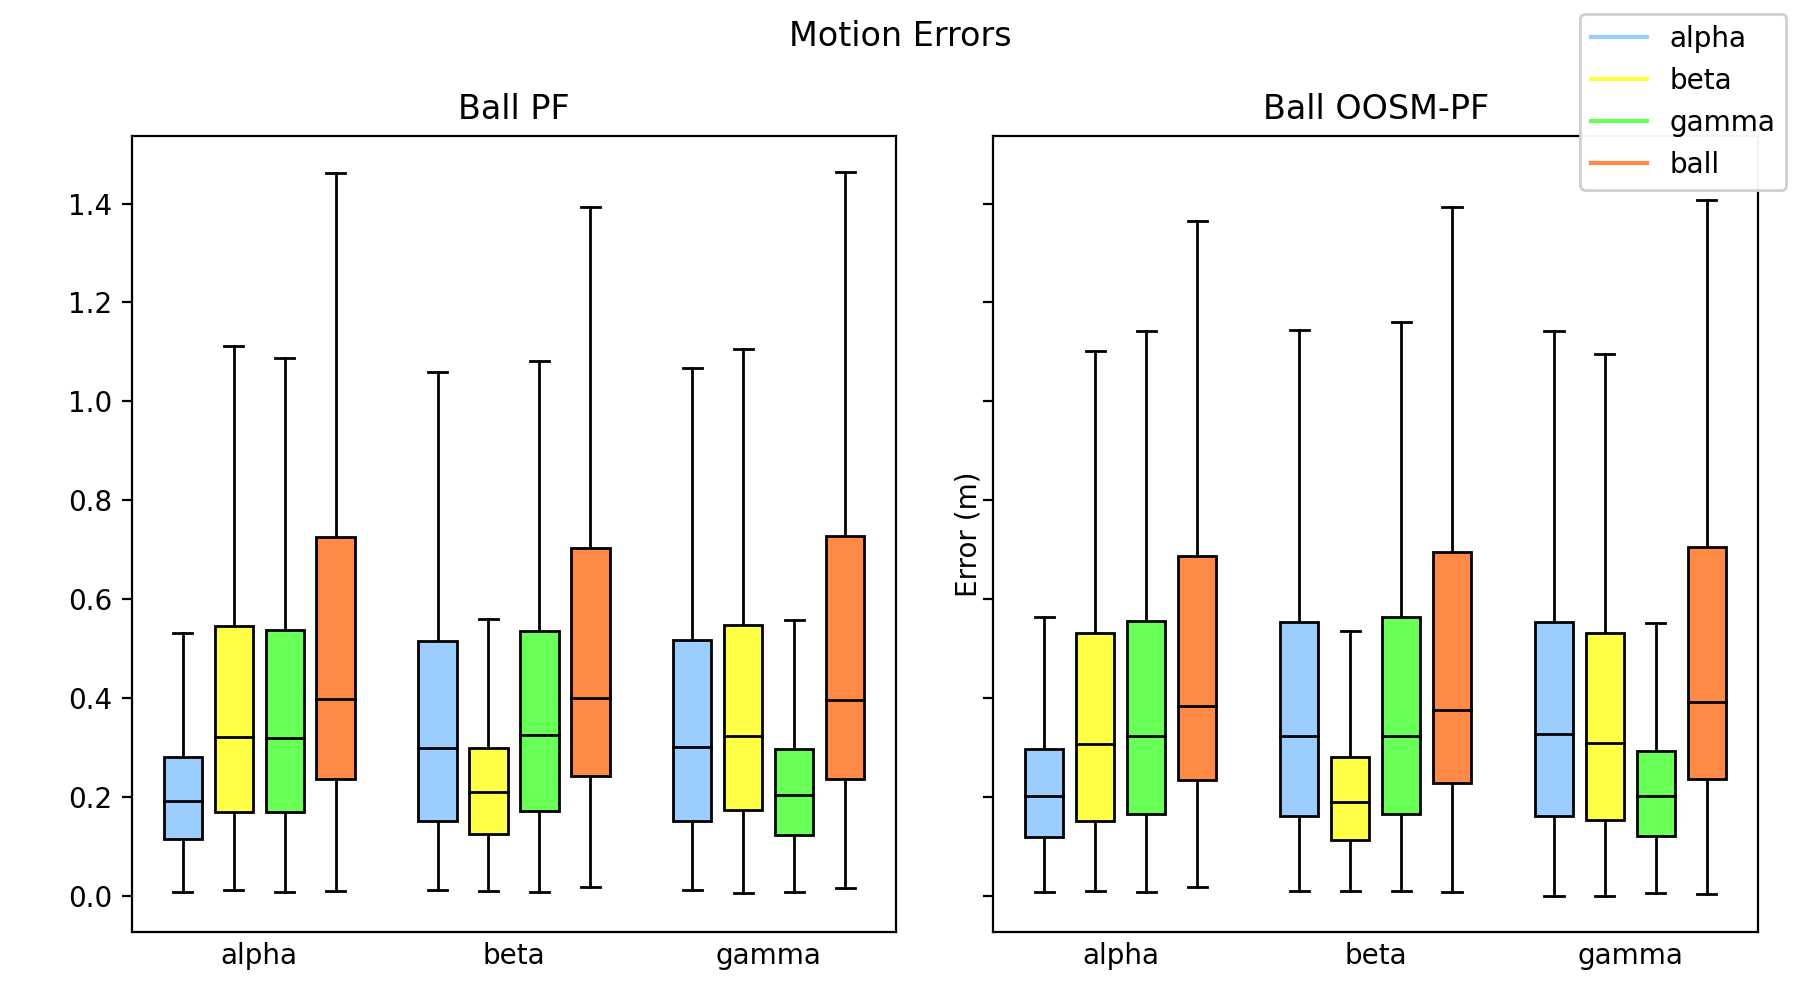
\includegraphics[width=0.9\textwidth]{resources/cfg2_AR_AS_error_motion.png}
    \caption{\textit{Error} \textit{world model} R dan S jaringan sedang}
    \label{fig:2-r-s-error}
    \bigskip
\end{figure}

\begin{figure}[p]
    \centering
    \medskip
    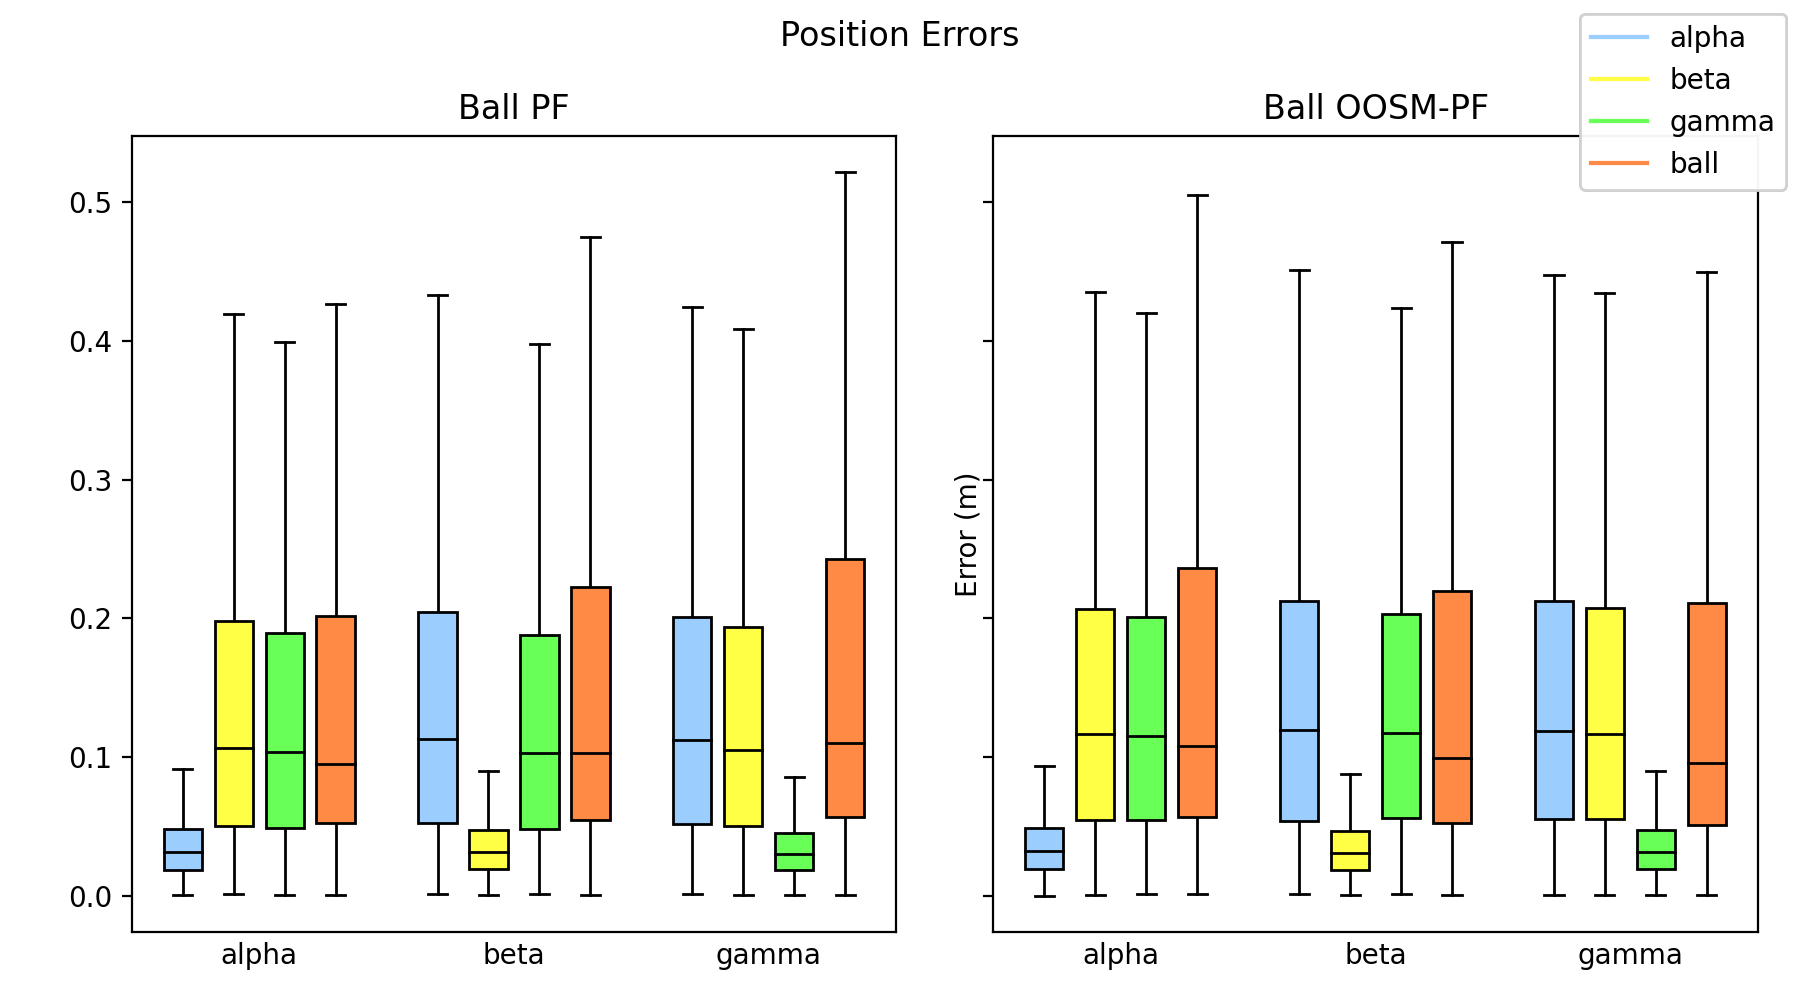
\includegraphics[width=0.9\textwidth]{resources/cfg3_AR_AS_error_pos.png}
    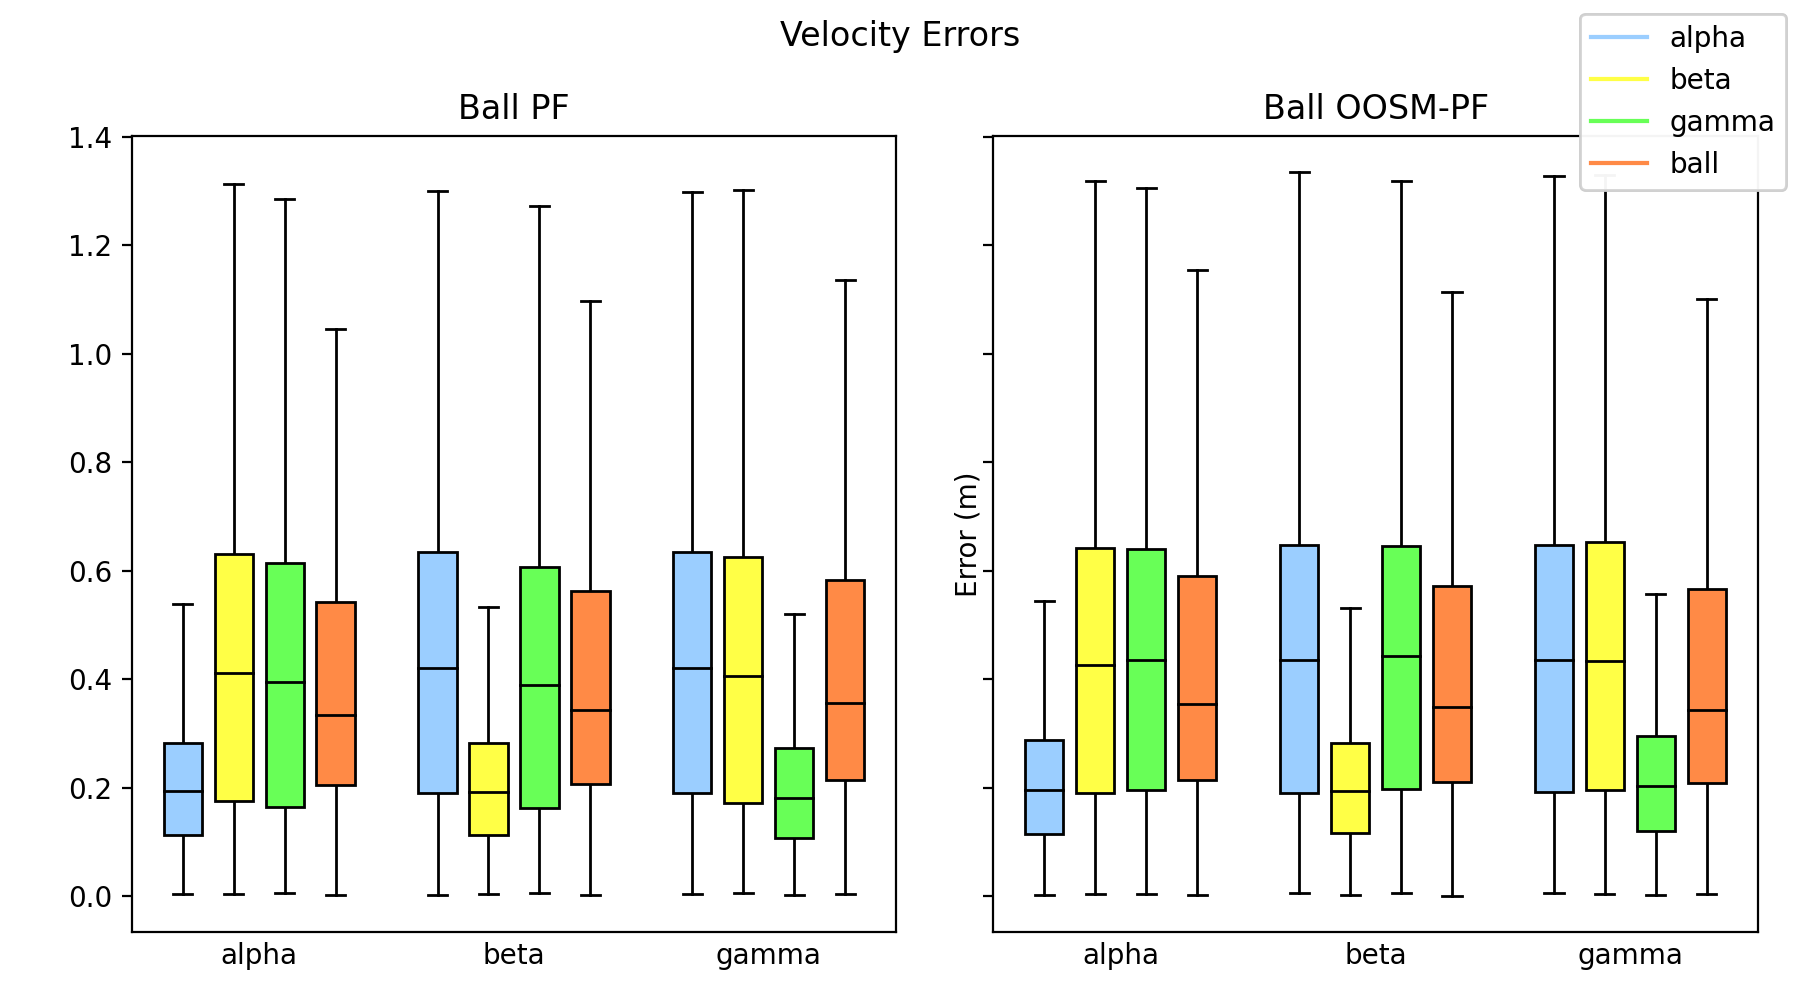
\includegraphics[width=0.9\textwidth]{resources/cfg3_AR_AS_error_vel.png}
    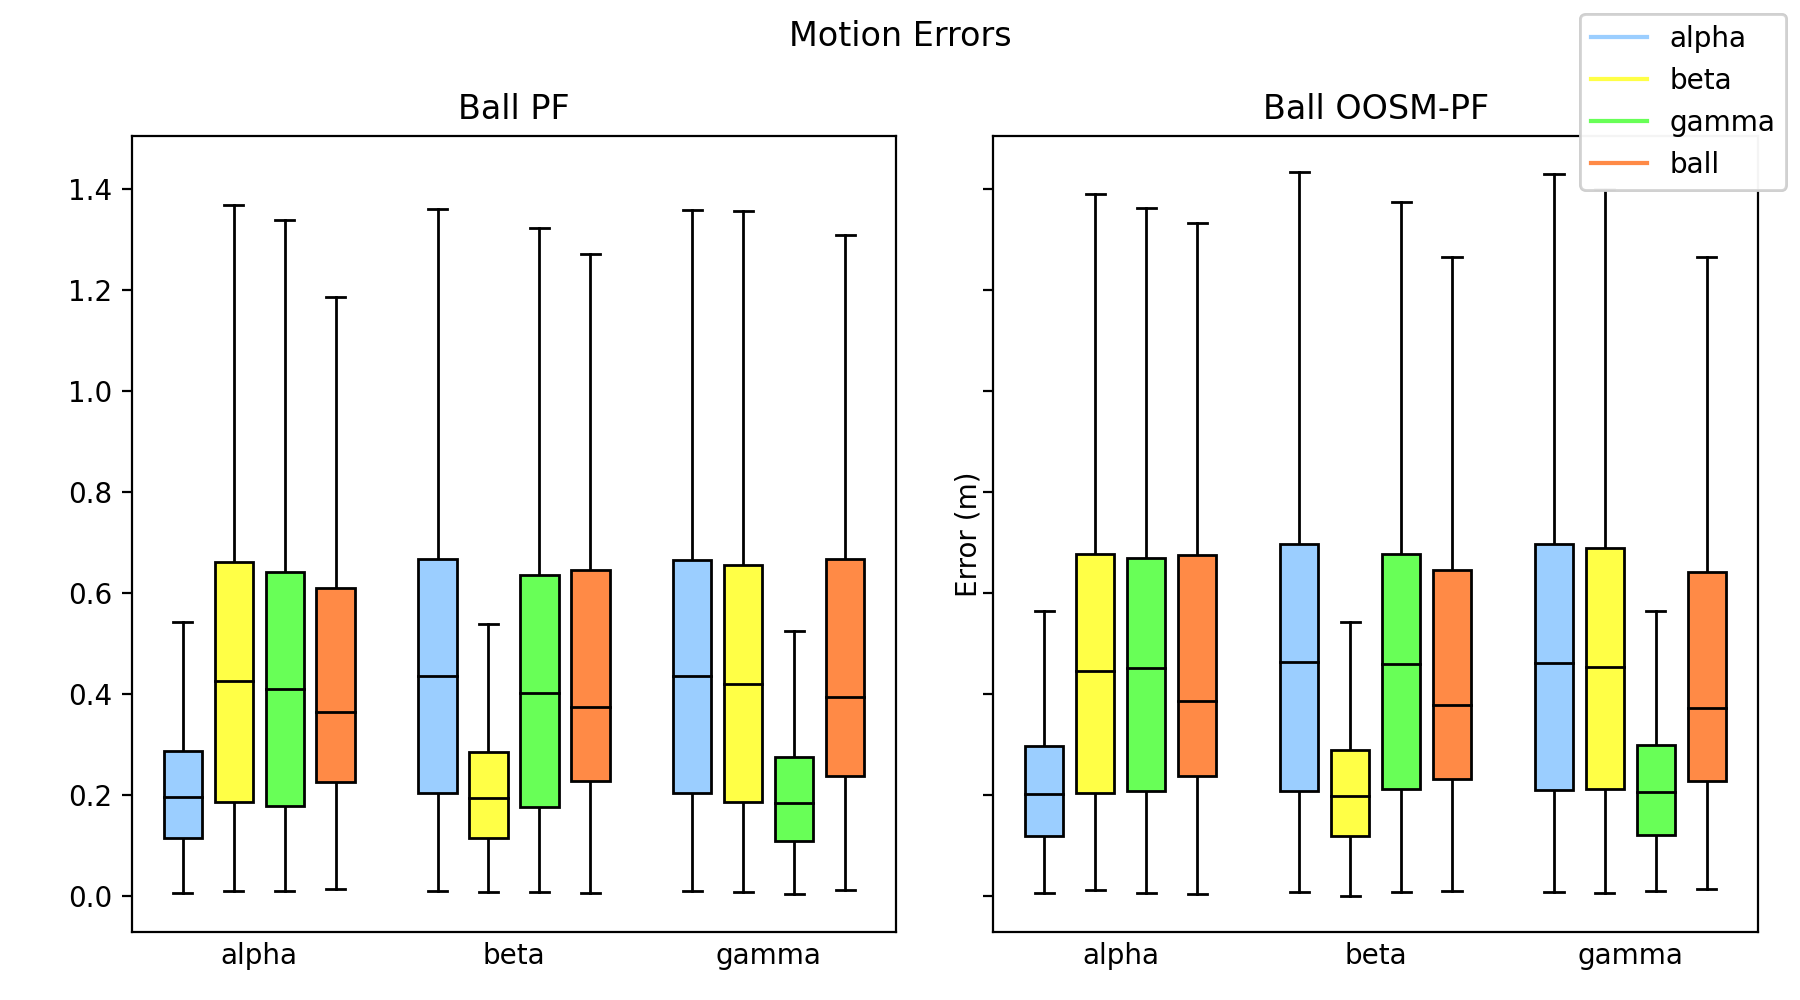
\includegraphics[width=0.9\textwidth]{resources/cfg3_AR_AS_error_motion.png}
    \caption{\textit{Error} \textit{world model} R dan S jaringan buruk}
    \label{fig:3-r-s-error}
    \bigskip
\end{figure}

Pada grafik \ref{fig:1-r-s-error}, terdapat peningkatan pada hasil estimasi posisi bola pada \textit{world model} yang menggunakan OOSM-PF saat jaringan baik, karena robot dapat mengintegrasi bacaan dari dua atau lebih robot yang melihat bola pada saat yang bersamaan untuk meningkatkan banyak data yang diintegrasi dan meningkatkan akurasi. Pada grafik \ref{fig:2-r-s-error} dan \ref{fig:3-r-s-error}, peningkatan ini semakin berkurang, karena pada saat robot dapat mengintegrasi data bola yang bersamaan dari dua robot atau lebih, data tersebut sudah cukup lama dan tidak lagi terlalu relevan terhadap hasil yang diestimasi sekarang.

\subsection{Perbandingan Algoritma Estimasi Bola tanpa Data Opsional dan dengan Data Opsional}

Dibandingkan dengan \textit{world model} S, \textit{world model} SB menggunakan OOSM-PF yang menerima data sensor yang dapat tidak melihat bola, daripada harus mengandung data bola yang terlihat.

\begin{figure}[p]
    \centering
    \medskip
    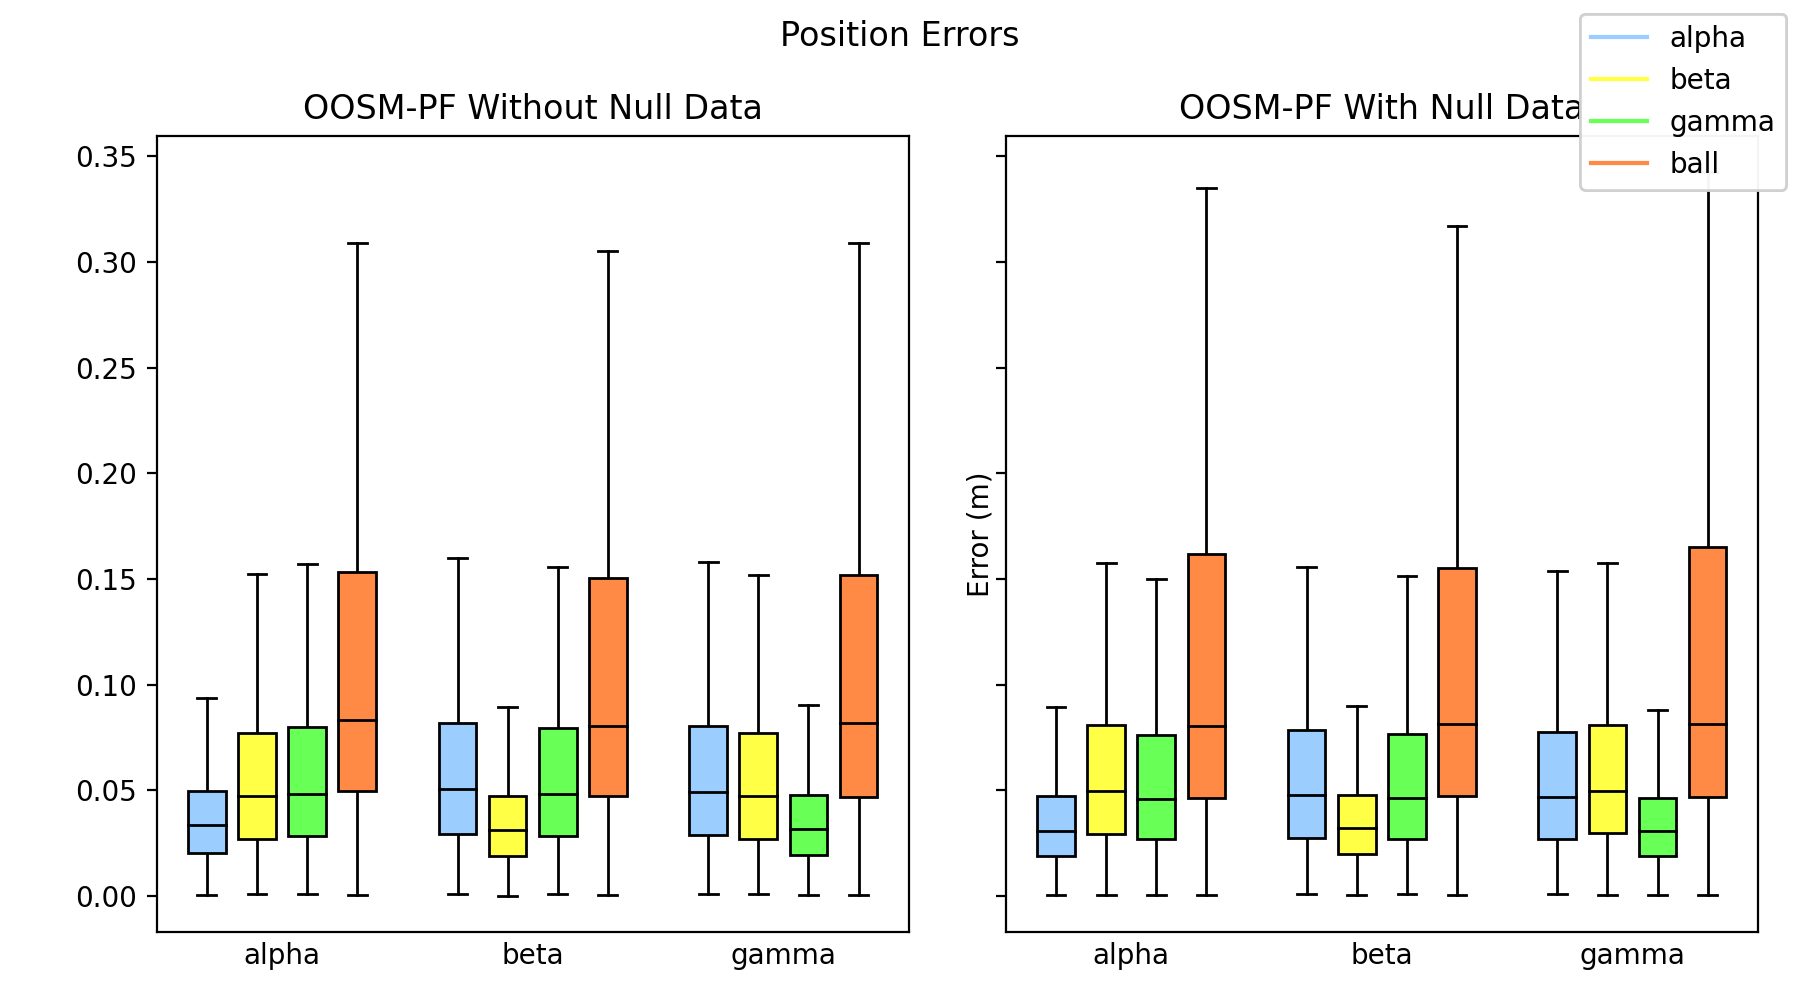
\includegraphics[width=0.9\textwidth]{resources/cfg1_AS_ASB_error_pos.png}
    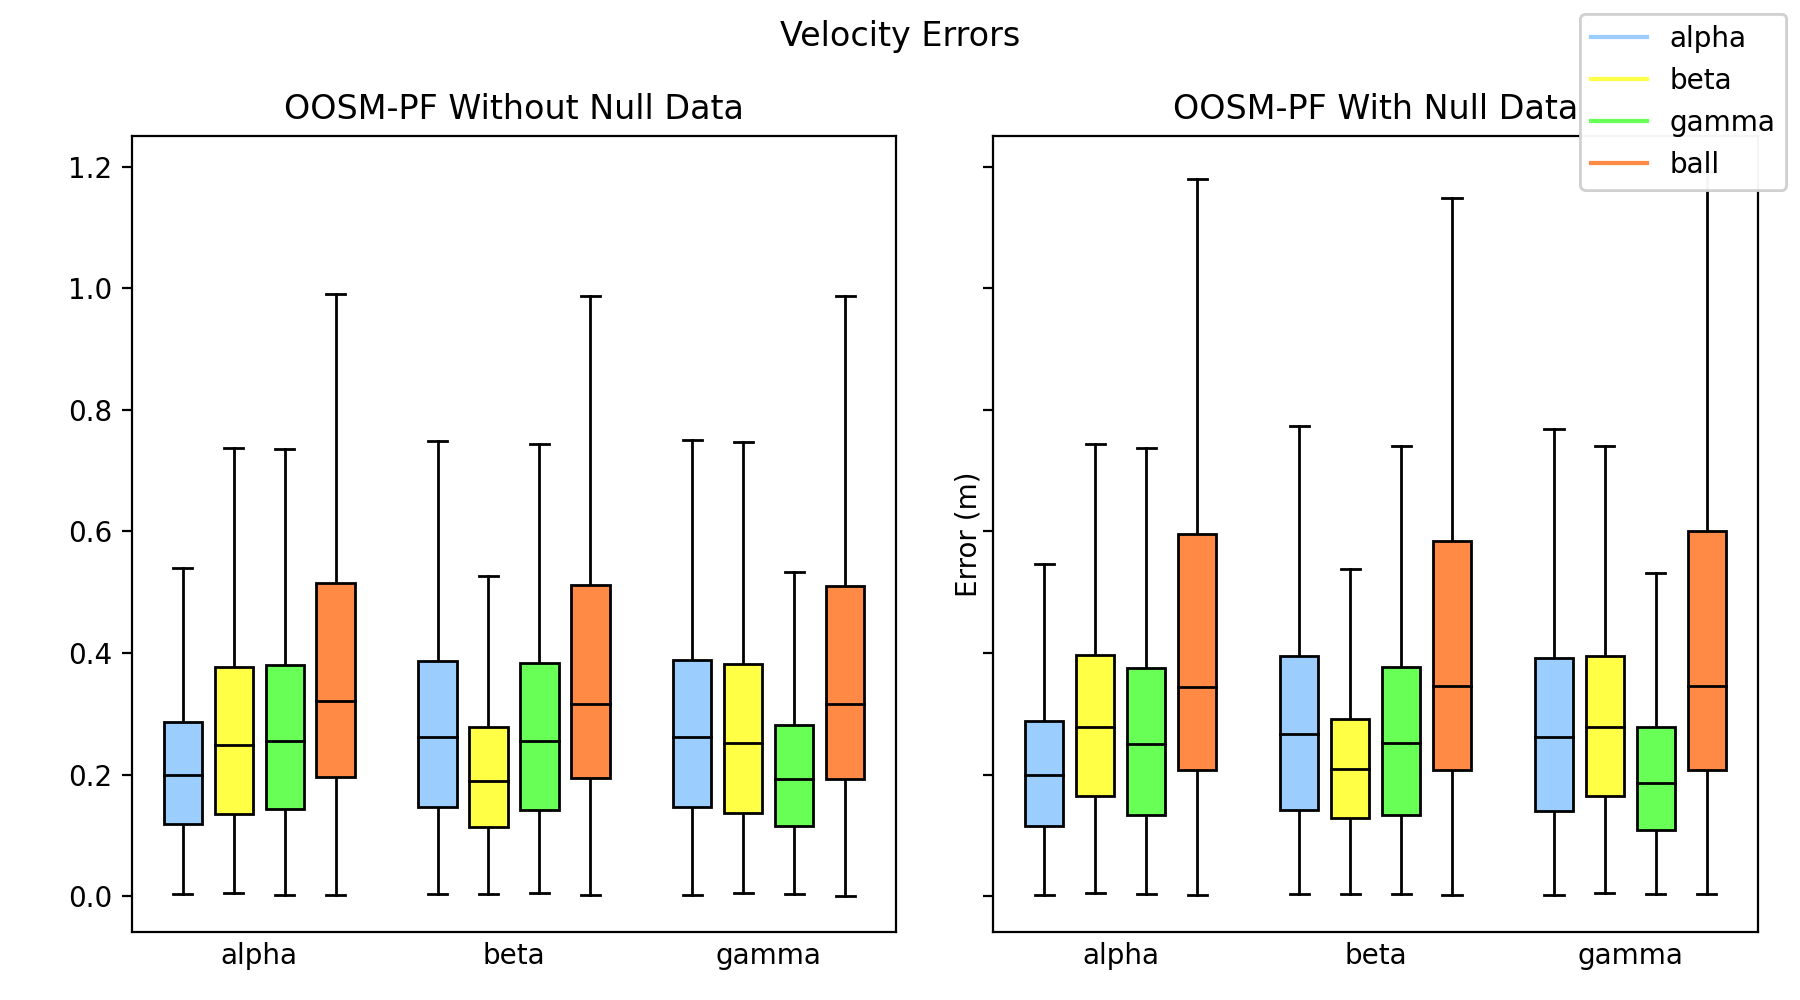
\includegraphics[width=0.9\textwidth]{resources/cfg1_AS_ASB_error_vel.png}
    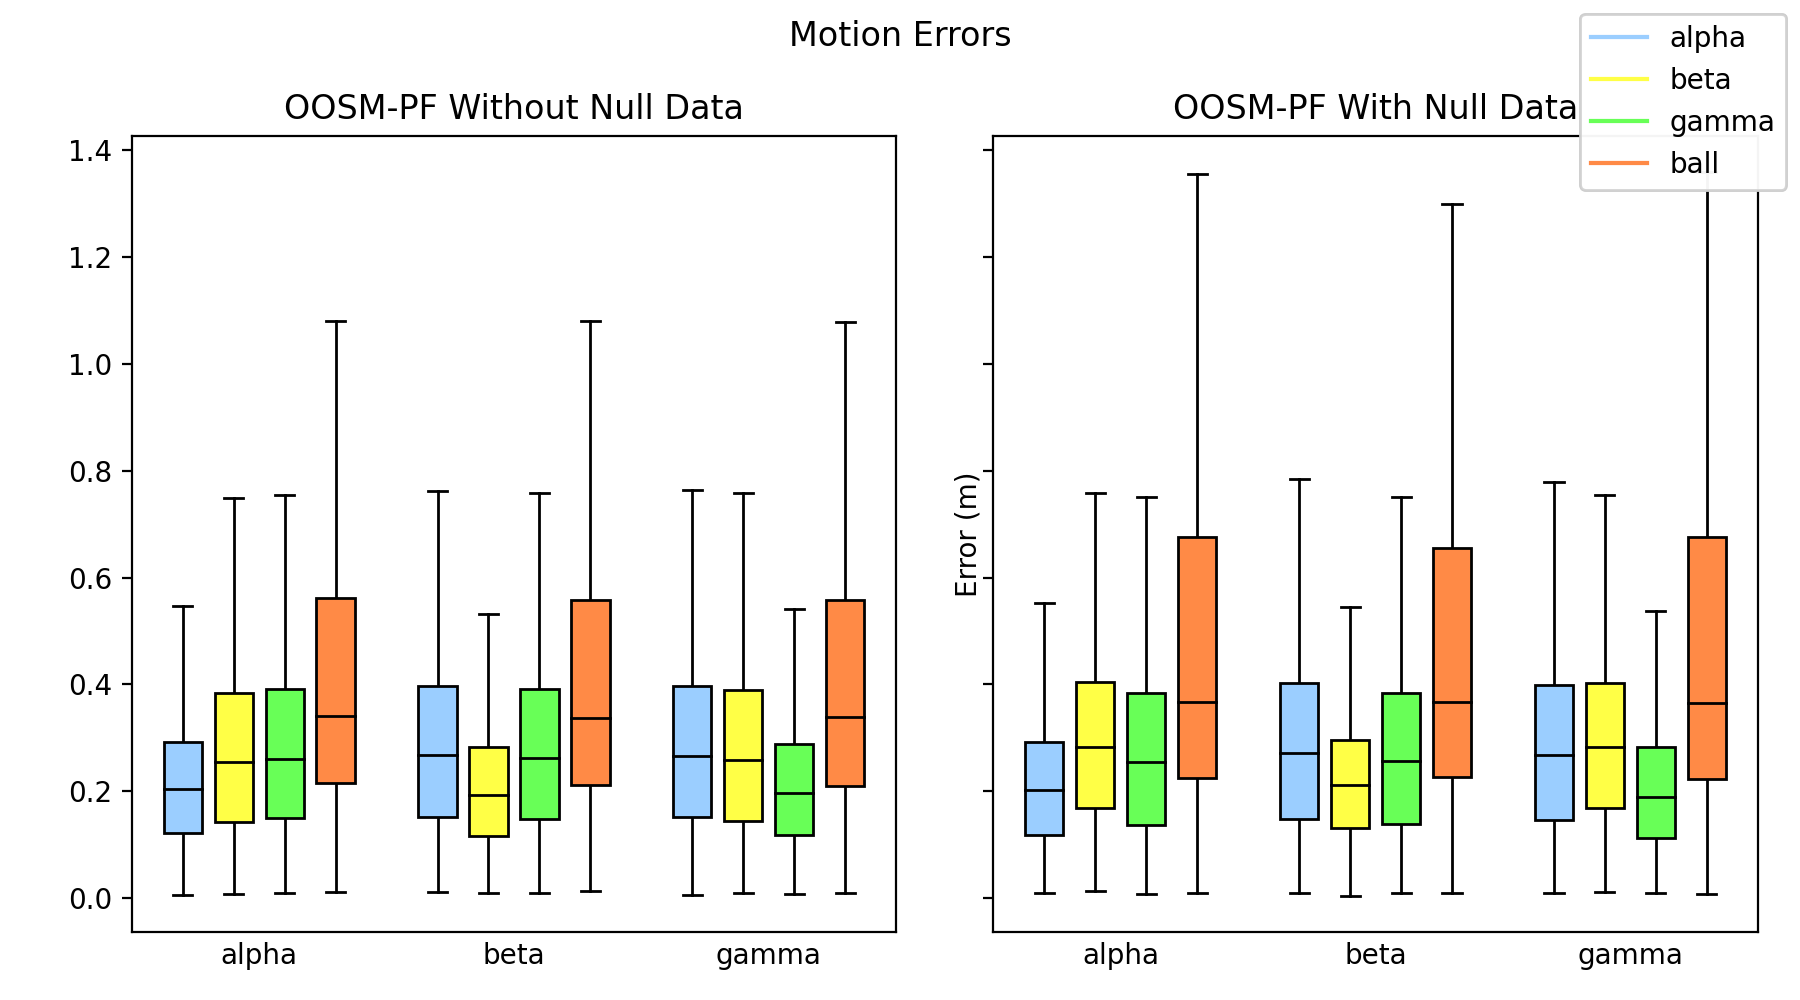
\includegraphics[width=0.9\textwidth]{resources/cfg1_AS_ASB_error_motion.png}
    \caption{\textit{Error} \textit{world model} S dan SB jaringan baik}
    \label{fig:1-s-sb-error}
    \bigskip
\end{figure}

Pada grafik \ref{fig:1-s-sb-error}, tidak ada perubahan yang signifikan dari integrasi data yang tidak \textit{null} untuk estimasi posisi dan malah memburuk untuk hasil estimasi kecepatan. Ini tampaknya disebabkan karena algoritma ini tidak mempertimbangkan saat bola tidak terlihat karena oklusi dari objek, sehingga saat bola tidak terlihat, partikel yang ada di luar lingkaran radius penglihatan punya berat yang lebih tinggi dan punya kecenderungan memiliki kecepatan yang lebih tinggi dalam menjauhi robot keluar dari lingkaran.

\subsection{Perbandingan Algoritma Estimasi Bola dengan OOSM-PF dan OOSM-KF}

Dibandingkan dengan \textit{world model} S, \textit{world model} SC menggunakan OOSM-KF yang berdasarkan algoritma penapis Kalman, daripada algoritma OOSM-PF yang berdasarkan algoritma penapis partikel.

\begin{figure}[p]
    \centering
    \medskip
    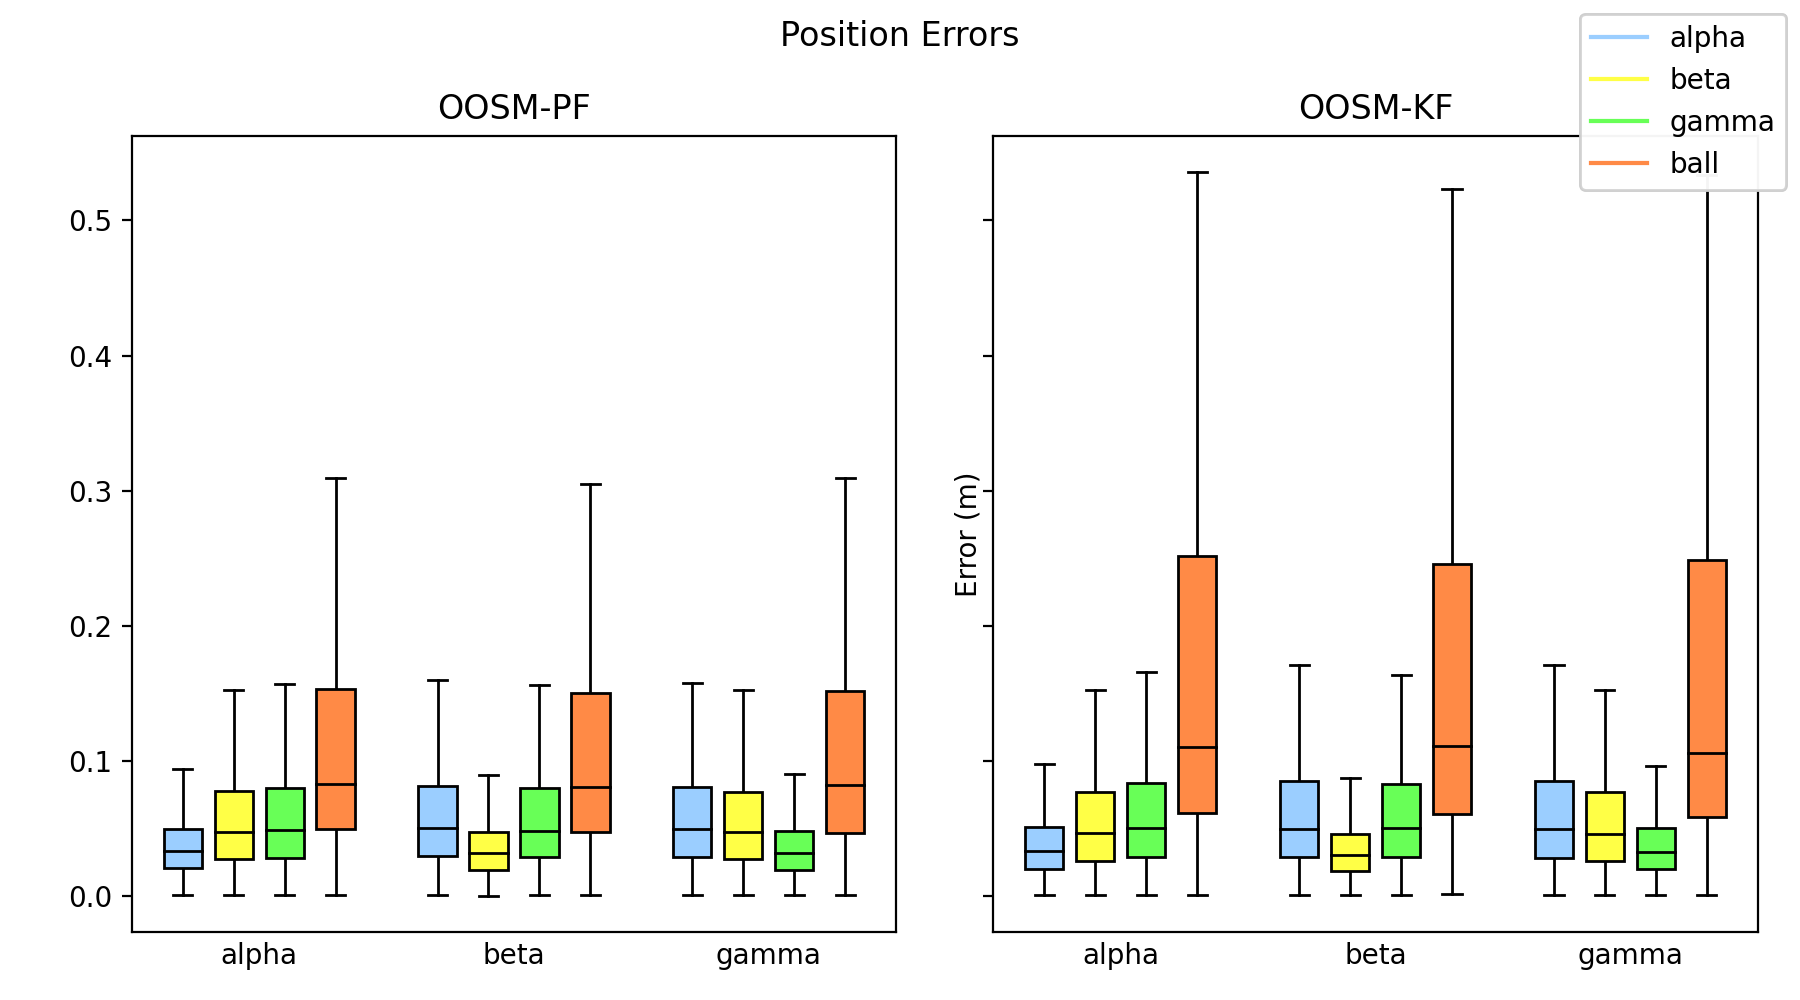
\includegraphics[width=0.9\textwidth]{resources/cfg1_AS_ASC_error_pos.png}
    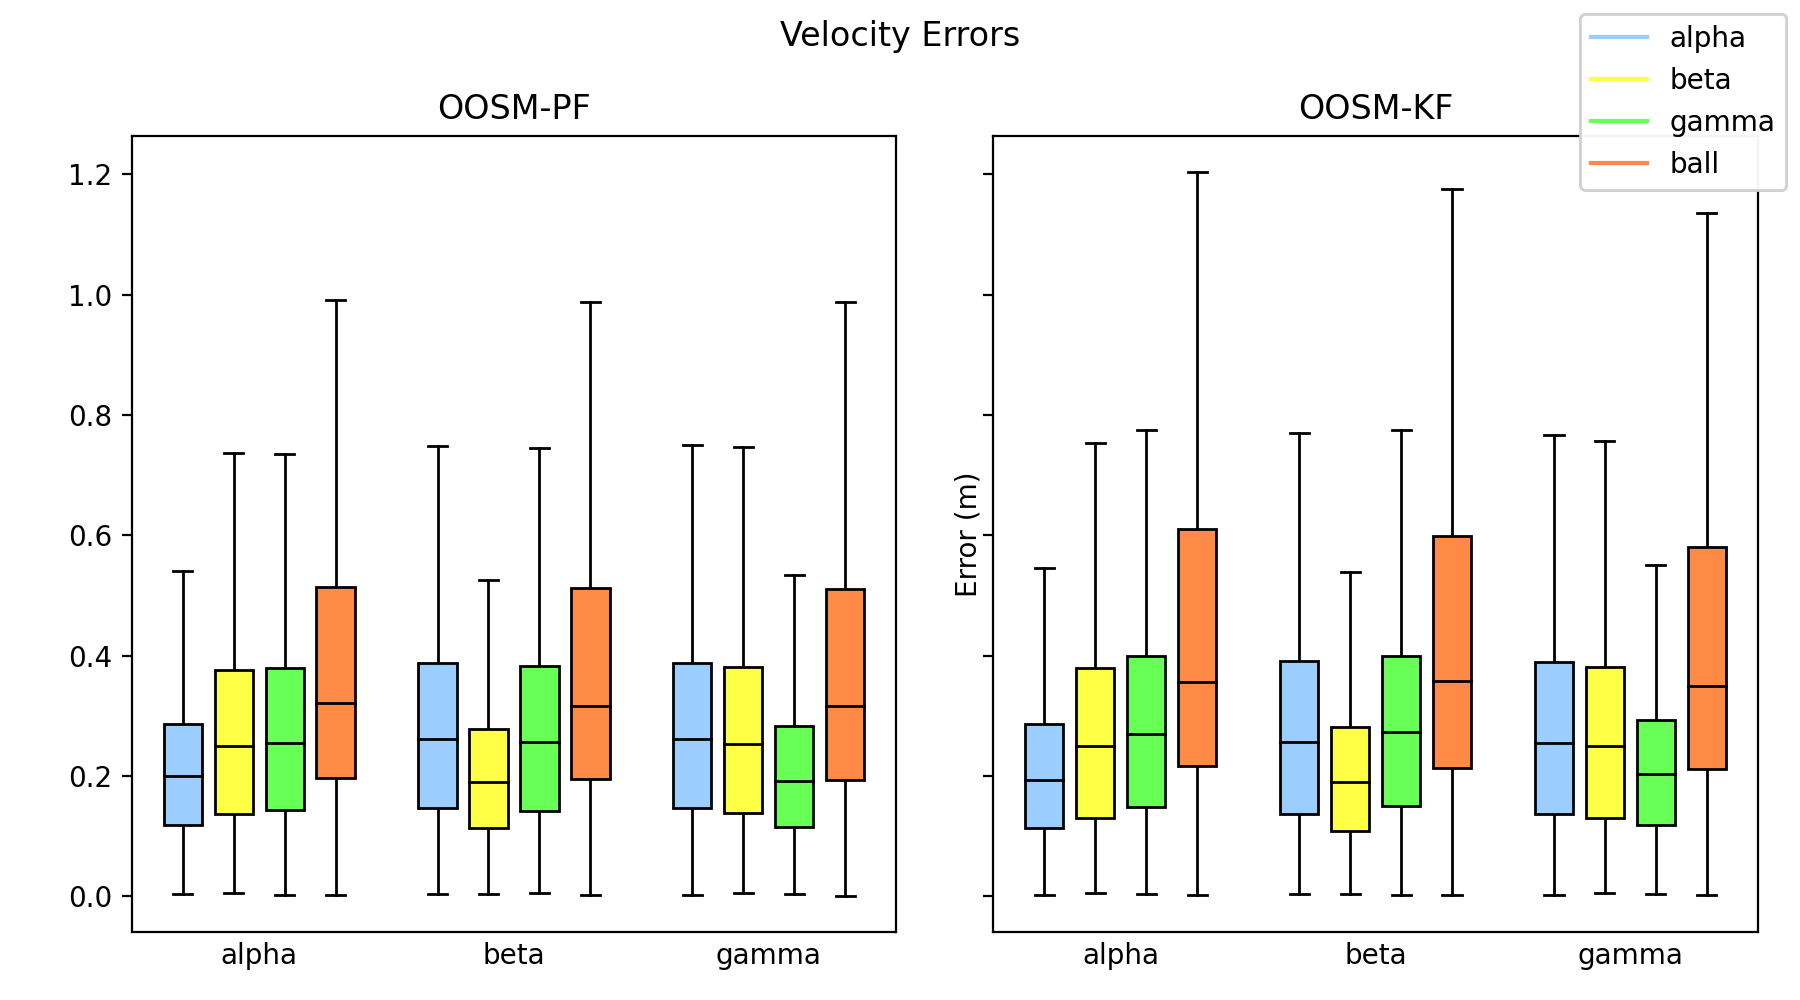
\includegraphics[width=0.9\textwidth]{resources/cfg1_AS_ASC_error_vel.png}
    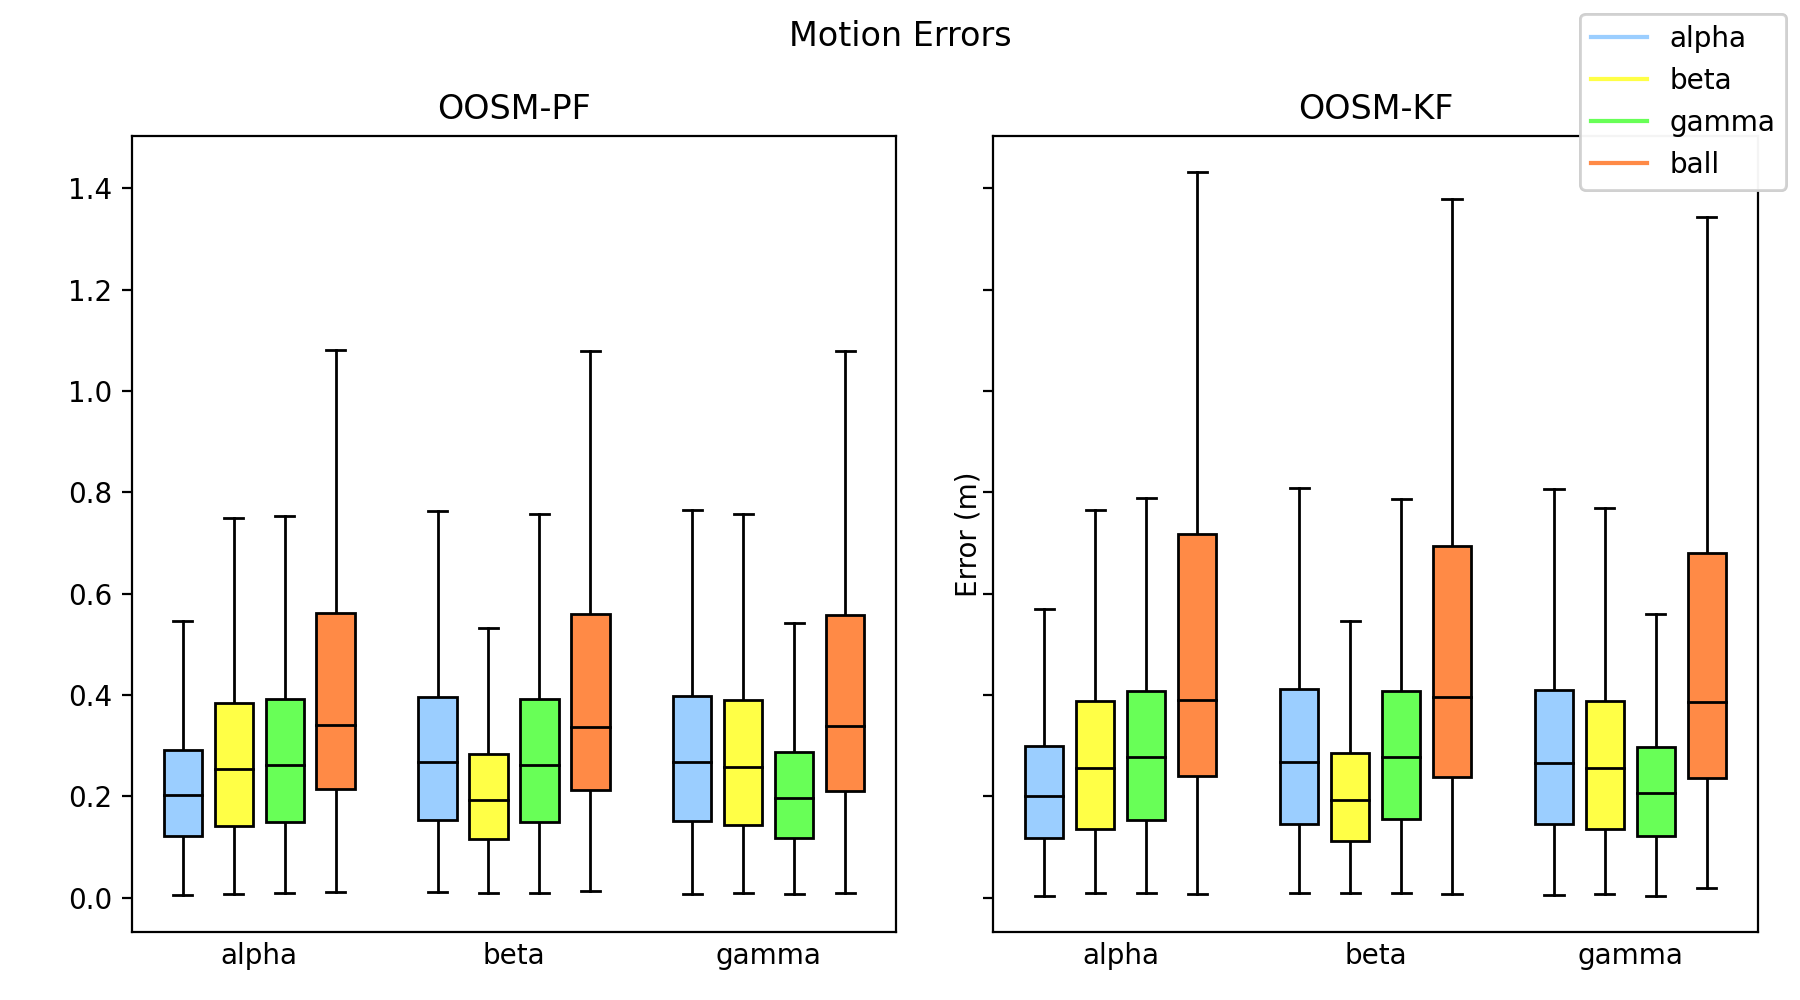
\includegraphics[width=0.9\textwidth]{resources/cfg1_AS_ASC_error_motion.png}
    \caption{\textit{Error} \textit{world model} S dan SC jaringan baik}
    \label{fig:1-s-sc-error}
    \bigskip
\end{figure}

Pada grafik \ref{fig:1-s-sc-error}, didapatkan \textit{error} estimasi posisi maupun kecepatan yang lebih buruk. Hal ini kemungkinan disebabkan oleh alasan yang sama dengan perbandingan kinerja PF dan KF dimana KF tidak dapat dengan sempurna memodelkan profil \textit{error} dari \textit{vision}, apalagi saat menggabungkan data dari sudut pandang dua atau lebih robot yang berbeda dengan arah distribusi \textit{error} yang berbeda juga.

\subsection{Perbandingan Algoritma Estimasi Bola OOSM-PF Biasa dan OOSM-KF dengan Kombinasi Data}

Dibandingkan dengan \textit{world model} S, \textit{world model} SD menggunakan OOSM-KF yang menggabungkan beberapa persepsi bola pada waktu yang sama dengan merata-ratakan posisinya.

\begin{figure}[p]
    \centering
    \medskip
    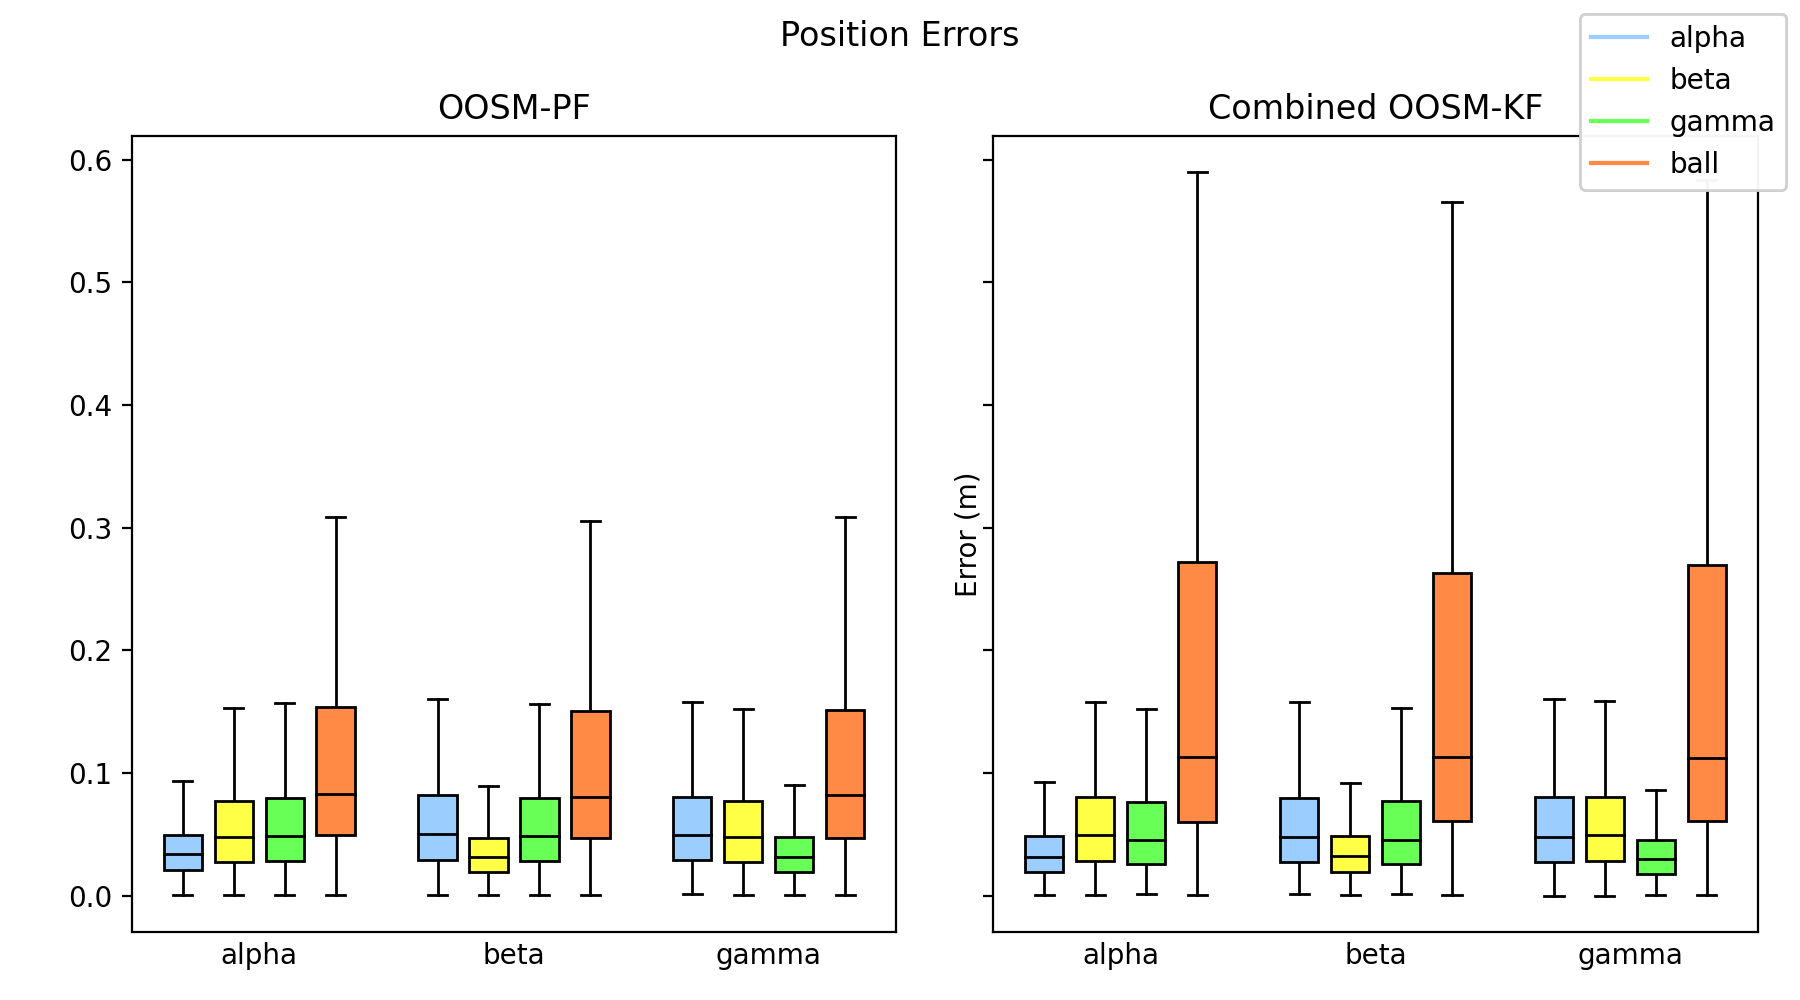
\includegraphics[width=0.9\textwidth]{resources/cfg1_AS_ASD_error_pos.png}
    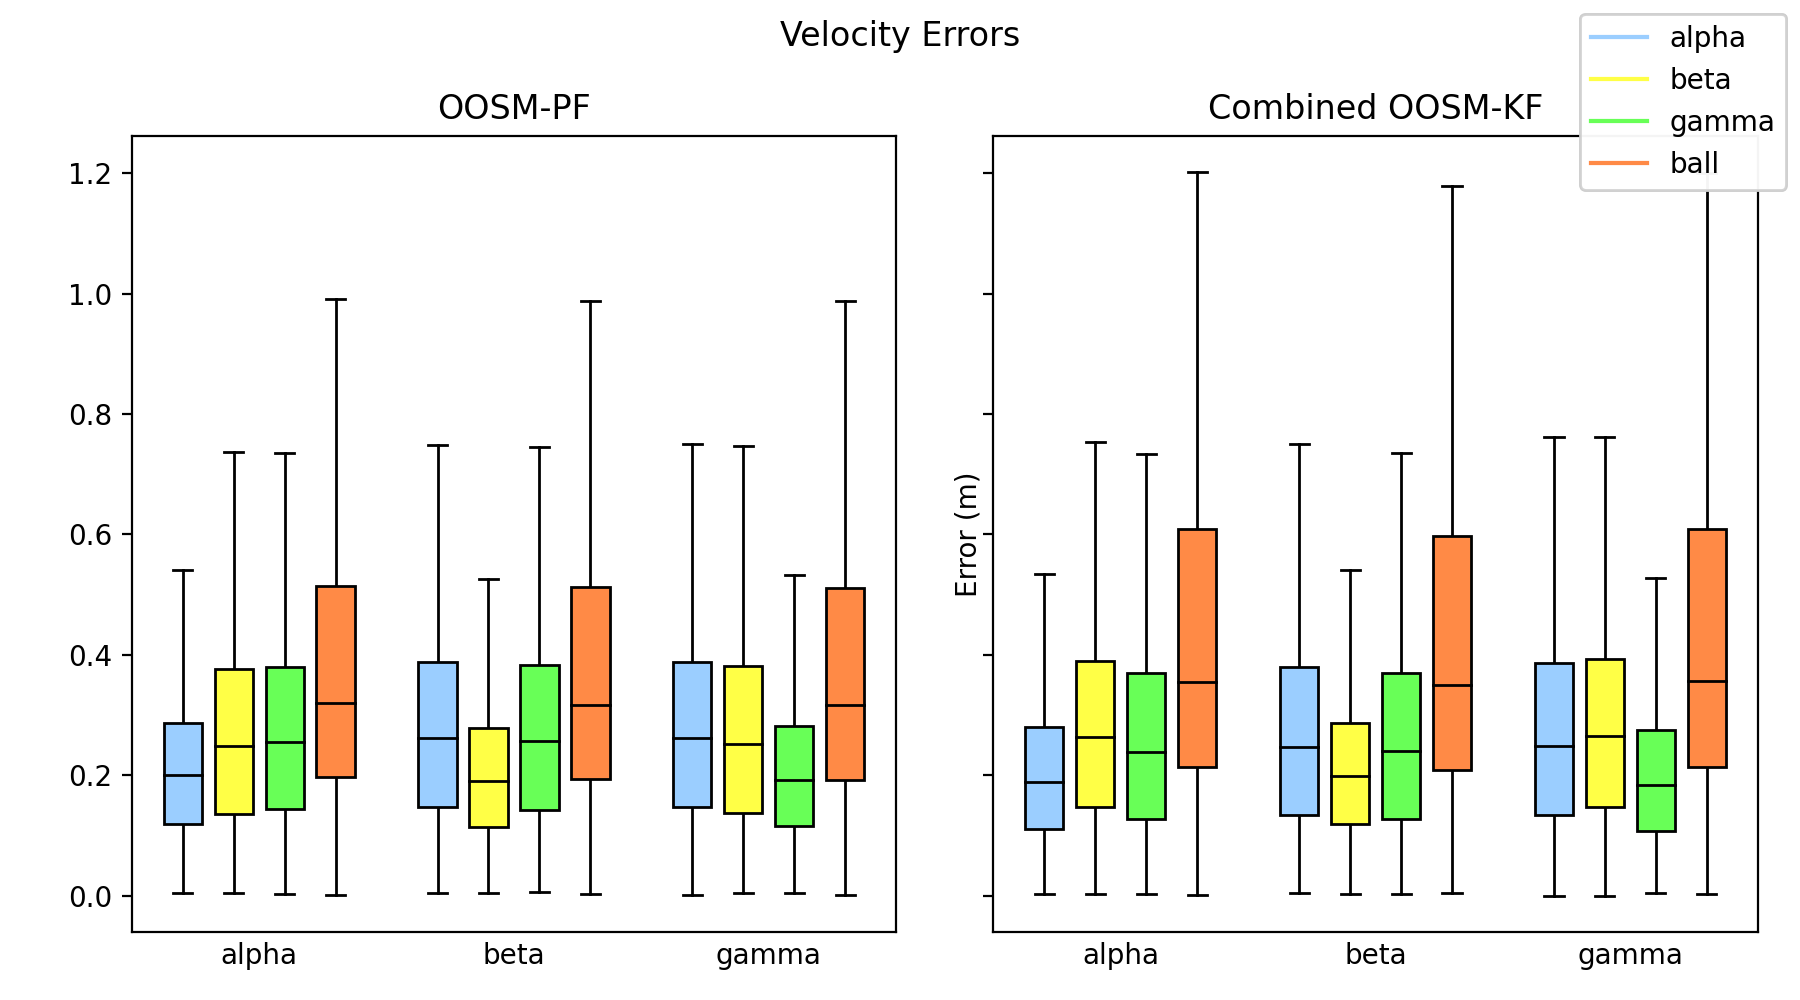
\includegraphics[width=0.9\textwidth]{resources/cfg1_AS_ASD_error_vel.png}
    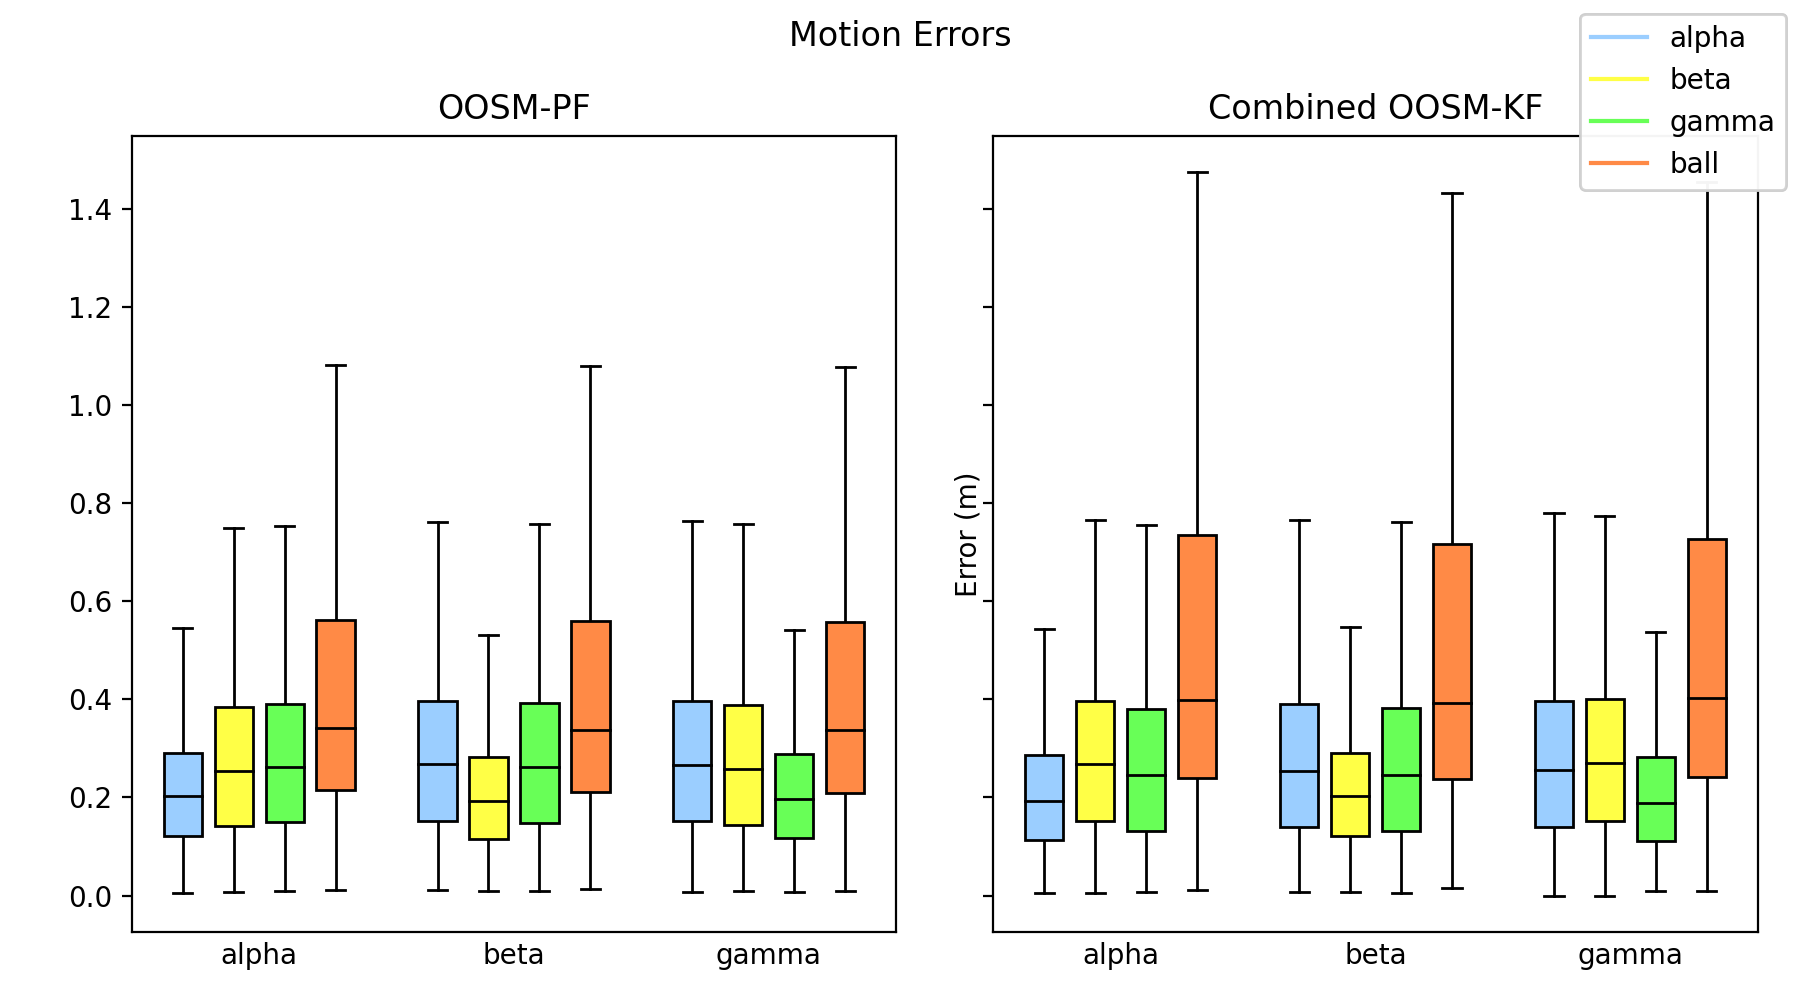
\includegraphics[width=0.9\textwidth]{resources/cfg1_AS_ASD_error_motion.png}
    \caption{\textit{Error} \textit{world model} S dan SD jaringan baik}
    \label{fig:1-s-sd-error}
    \bigskip
\end{figure}

Pada grafik \ref{fig:1-s-sd-error}, didapatkan \textit{error} estimasi posisi maupun kecepatan yang lebih buruk, dan kinerja \textit{world model} SD yang tidak jauh dari SC, yang kemungkinan dikarenakan oleh alasan yang sama dimana penggunaan OOSM-KFnya tidak cocok untuk profil \textit{error} \textit{vision} yang ada.

\subsection{Perbandingan Algoritma tanpa dan dengan Koreksi Posisi Robot Teman}

Dibandingkan dengan \textit{world model} S, \textit{world model} T mengoreksi posisi teman yang diterima dari komunikasi menggunakan persepsi sendiri dari \textit{vision}.

\begin{figure}[p]
    \centering
    \medskip
    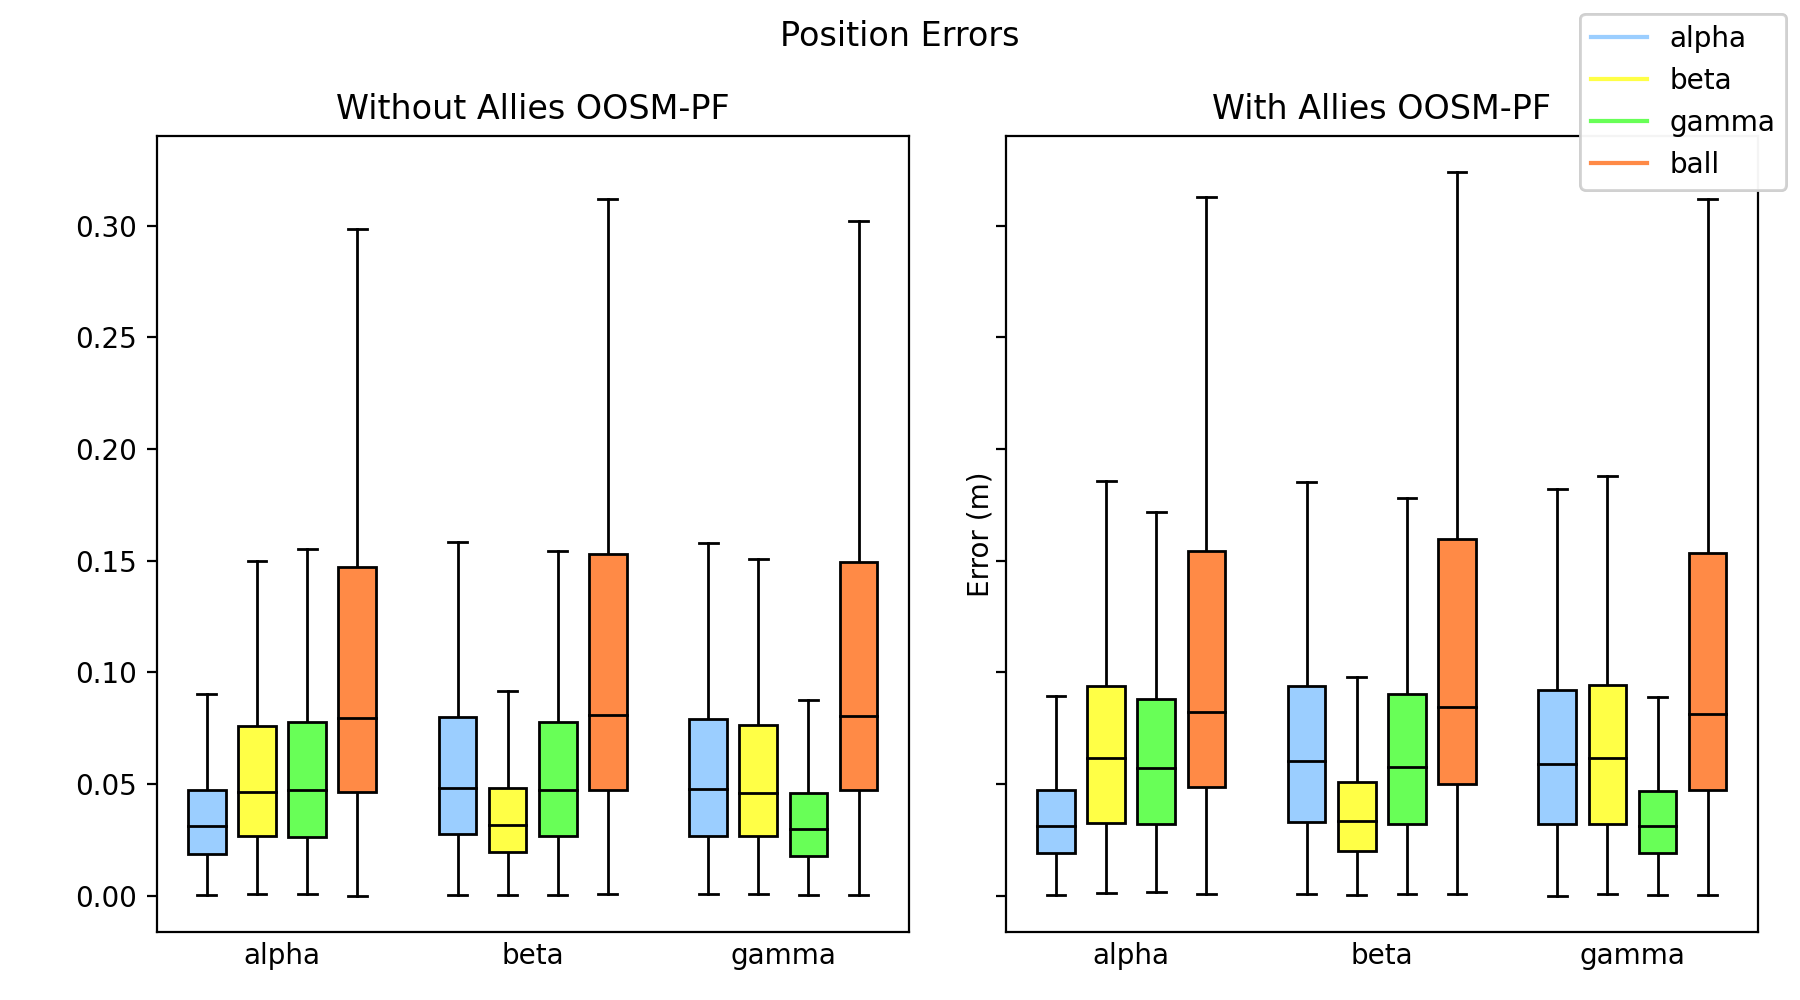
\includegraphics[width=0.9\textwidth]{resources/cfg1_AS_AT_error_pos.png}
    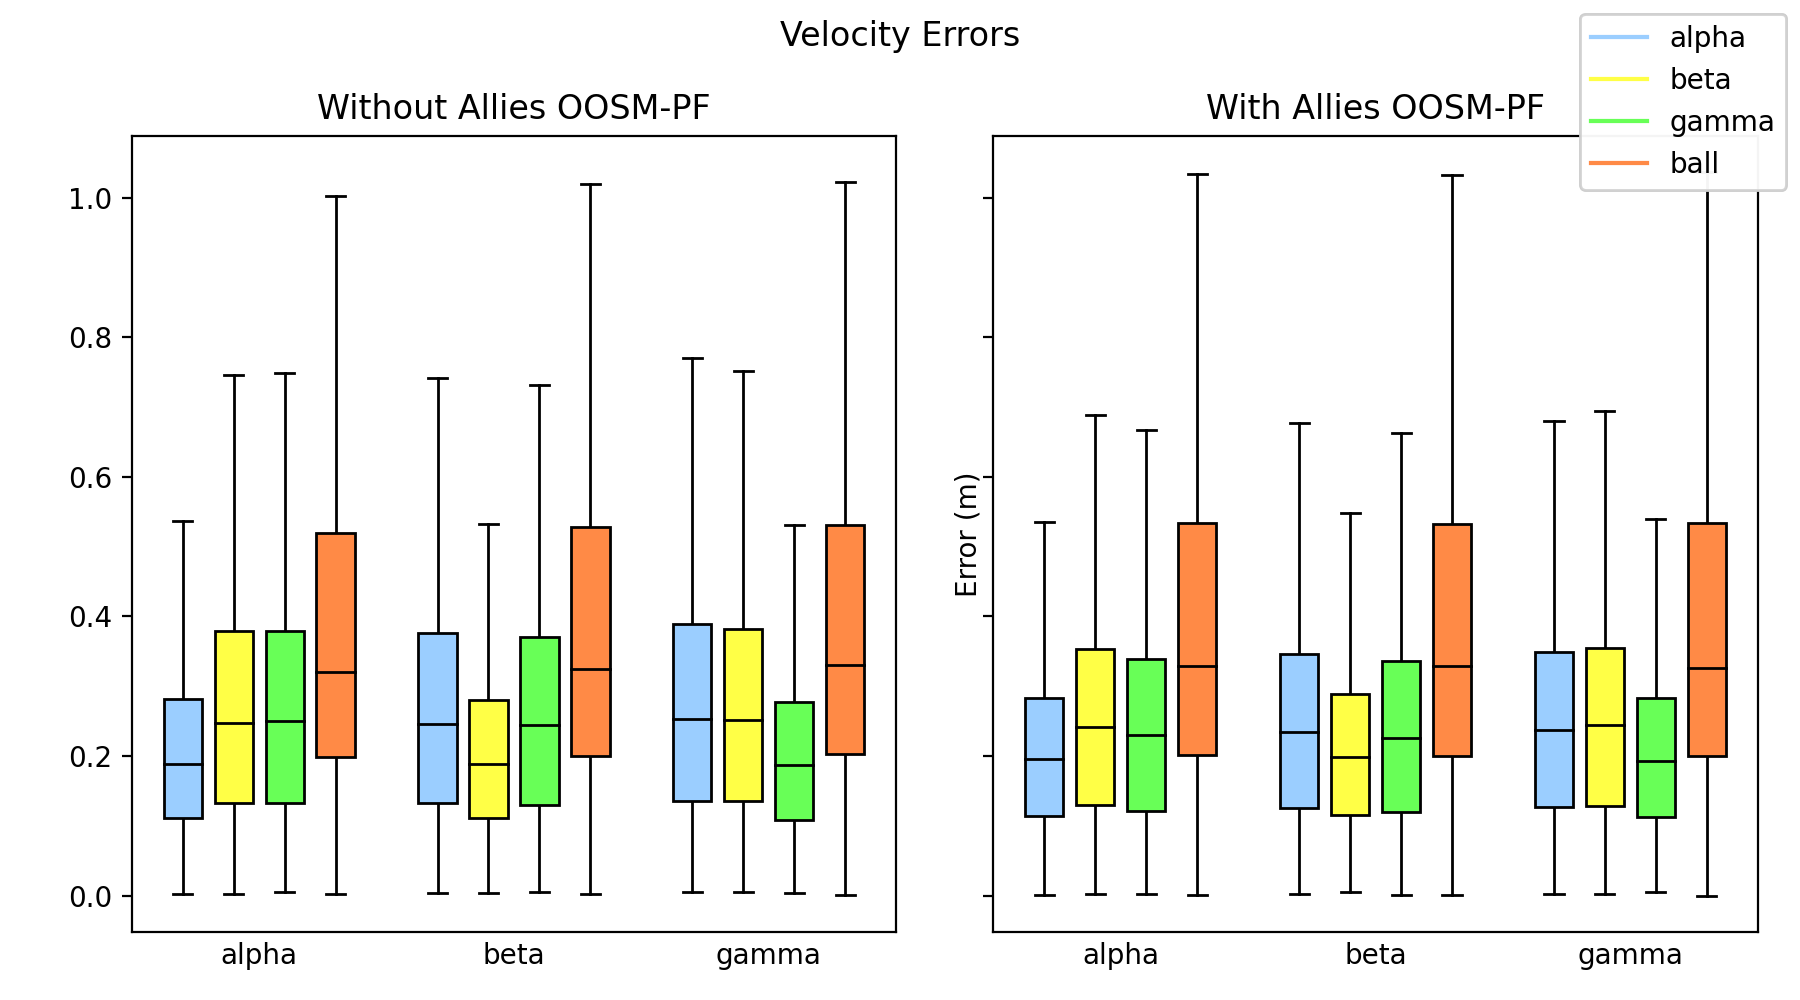
\includegraphics[width=0.9\textwidth]{resources/cfg1_AS_AT_error_vel.png}
    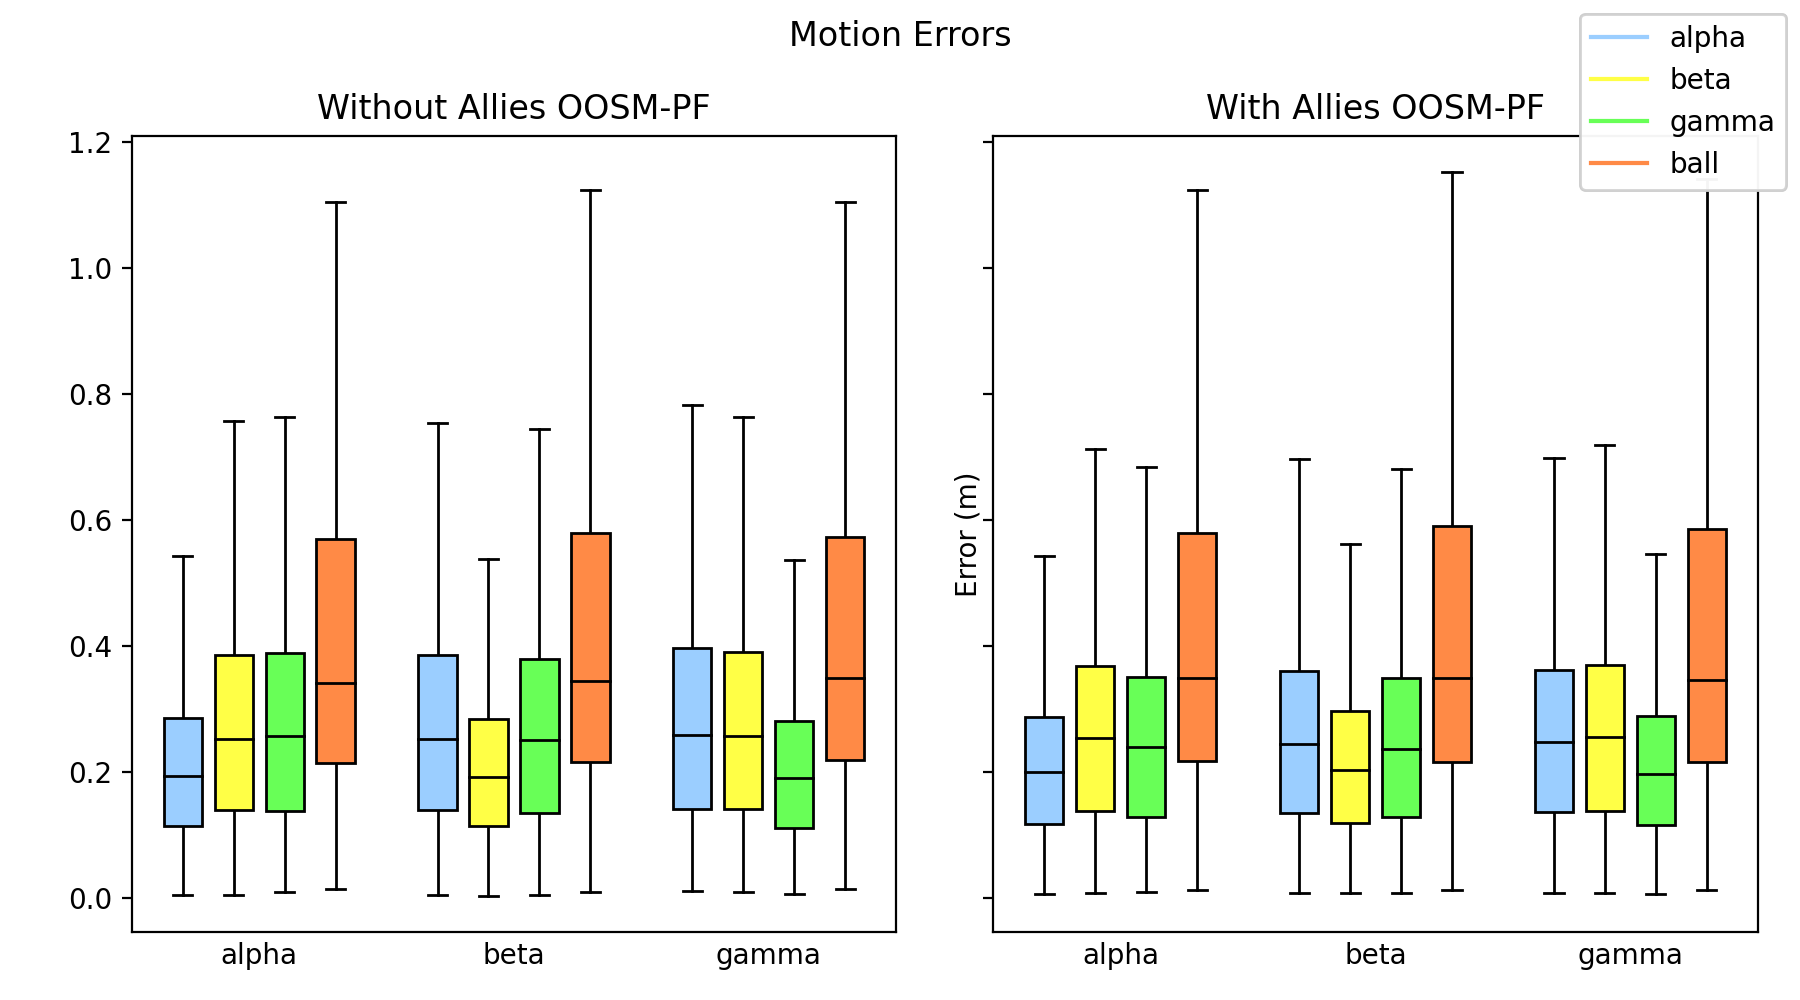
\includegraphics[width=0.9\textwidth]{resources/cfg1_AS_AT_error_motion.png}
    \caption{\textit{Error} \textit{world model} S dan T jaringan baik}
    \label{fig:1-s-t-error}
    \bigskip
\end{figure}

\begin{figure}[p]
    \centering
    \medskip
    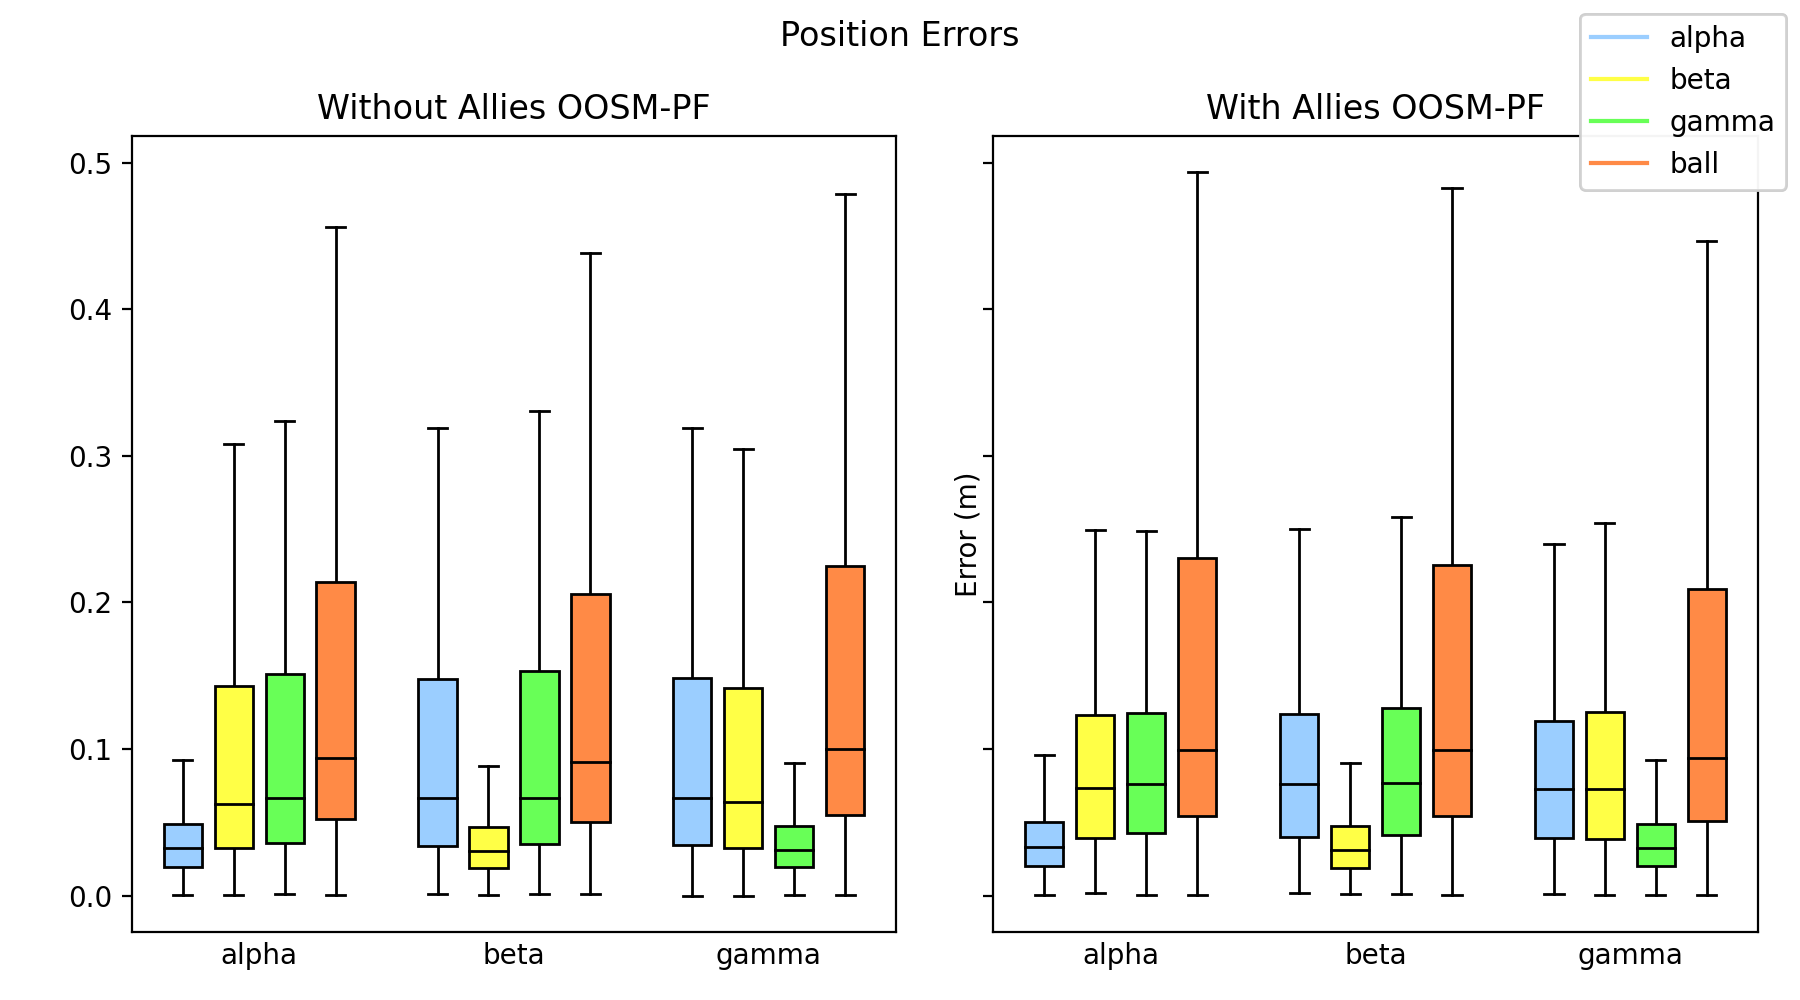
\includegraphics[width=0.9\textwidth]{resources/cfg2_AS_AT_error_pos.png}
    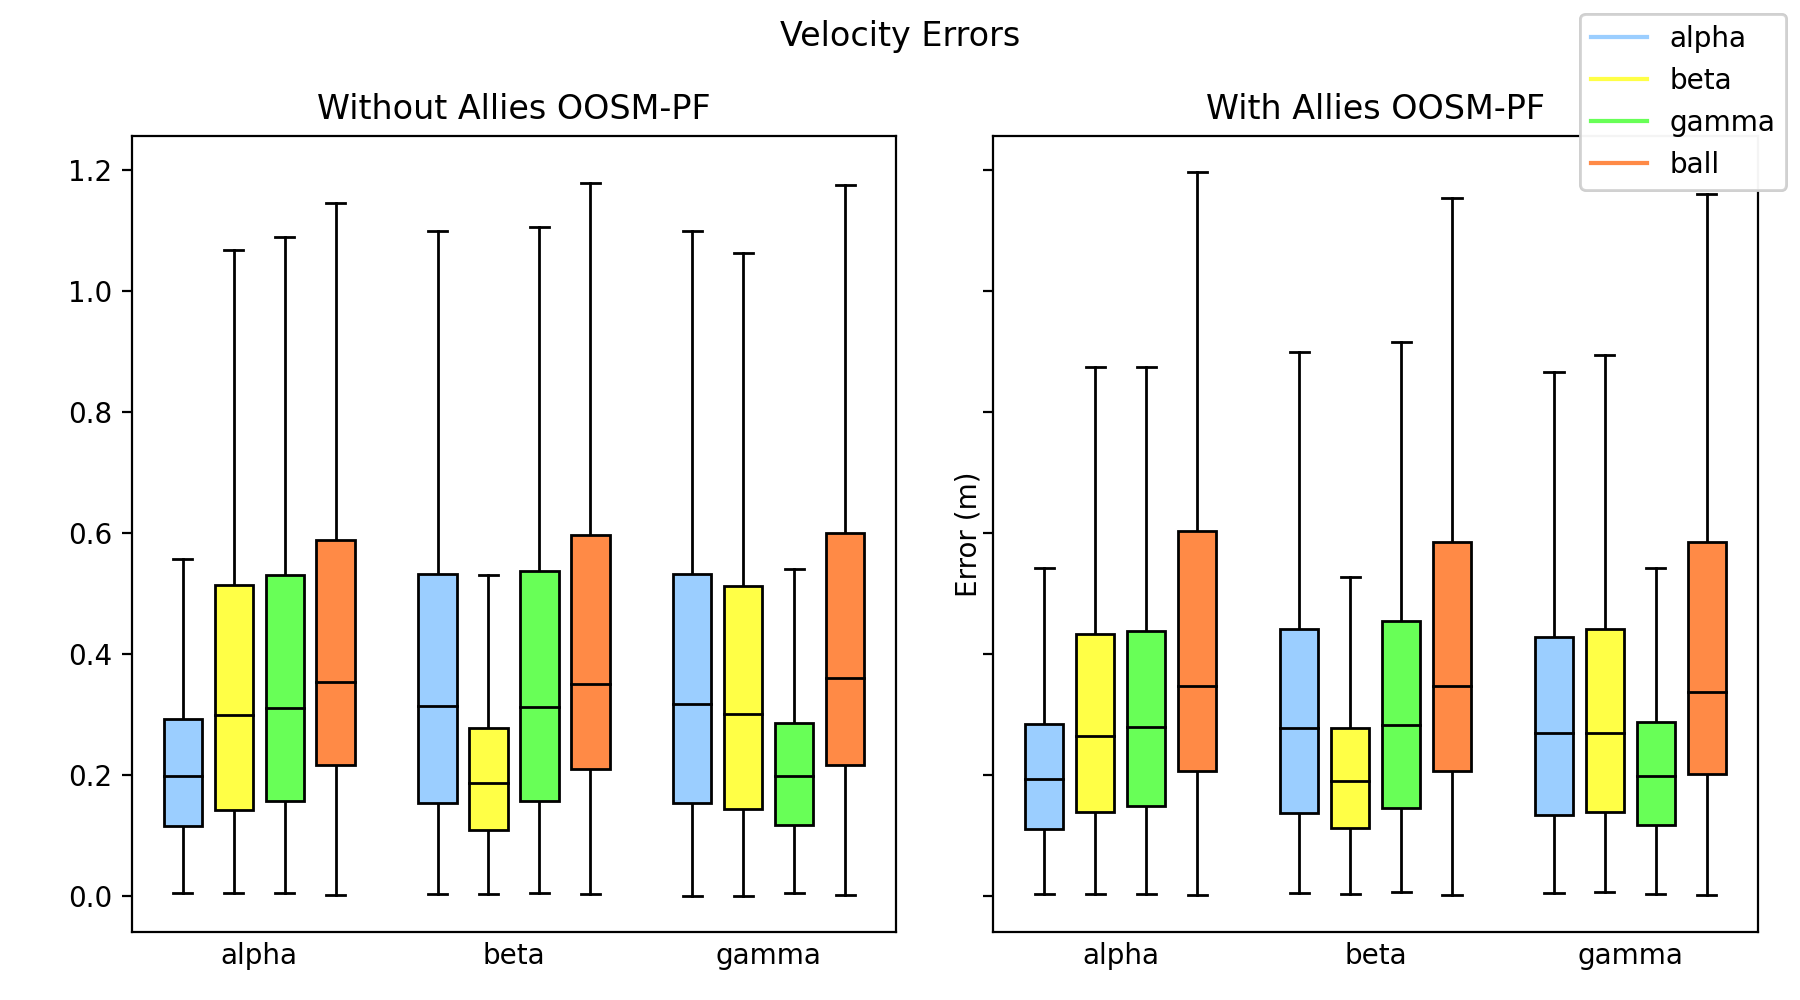
\includegraphics[width=0.9\textwidth]{resources/cfg2_AS_AT_error_vel.png}
    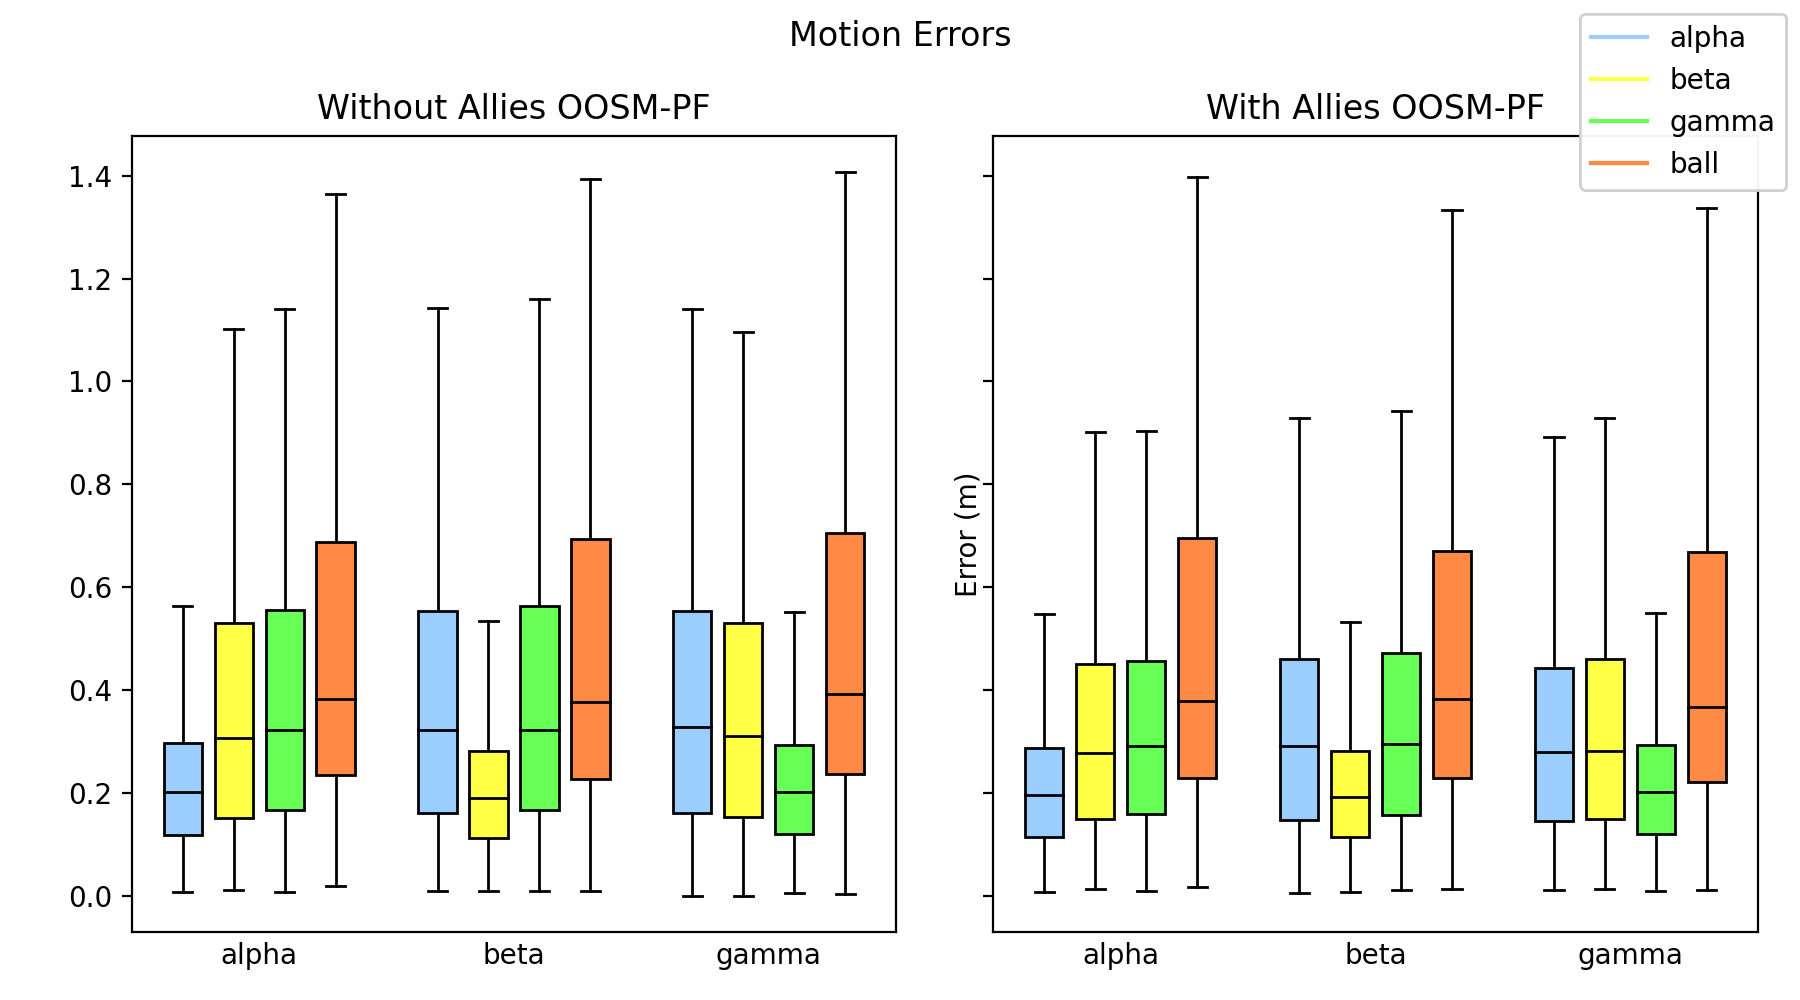
\includegraphics[width=0.9\textwidth]{resources/cfg2_AS_AT_error_motion.png}
    \caption{\textit{Error} \textit{world model} S dan T jaringan sedang}
    \label{fig:2-s-t-error}
    \bigskip
\end{figure}

\begin{figure}[p]
    \centering
    \medskip
    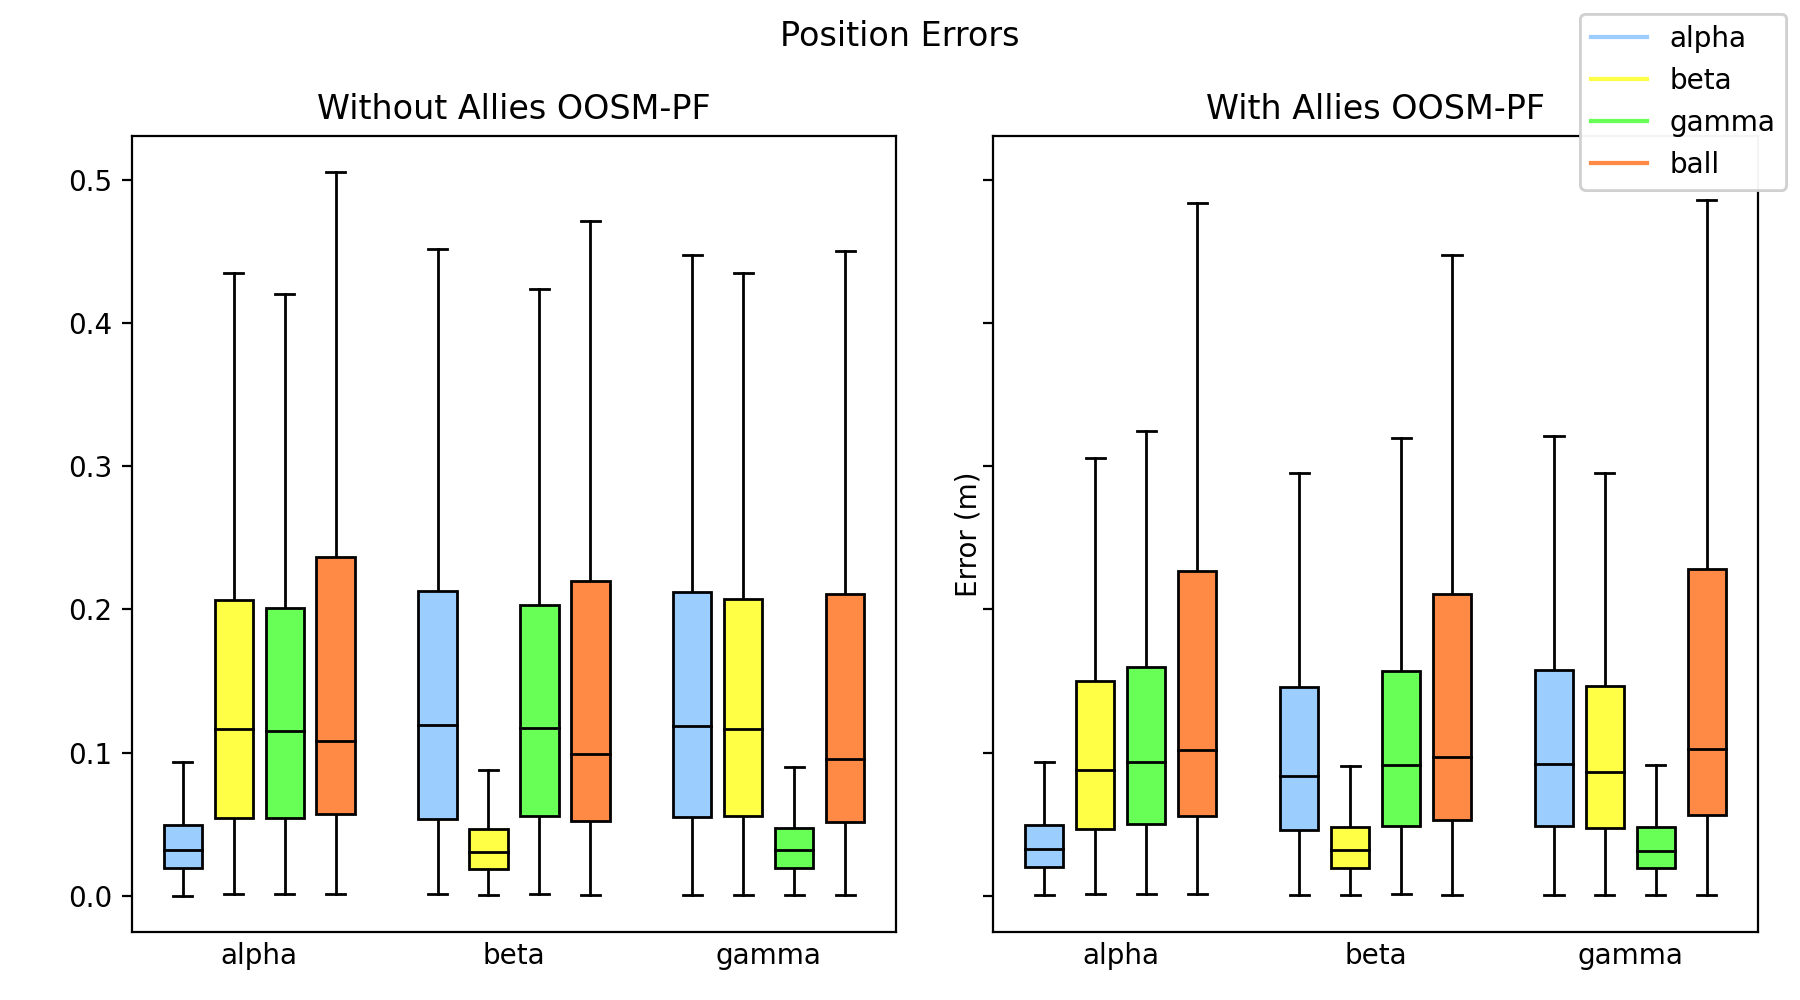
\includegraphics[width=0.9\textwidth]{resources/cfg3_AS_AT_error_pos.png}
    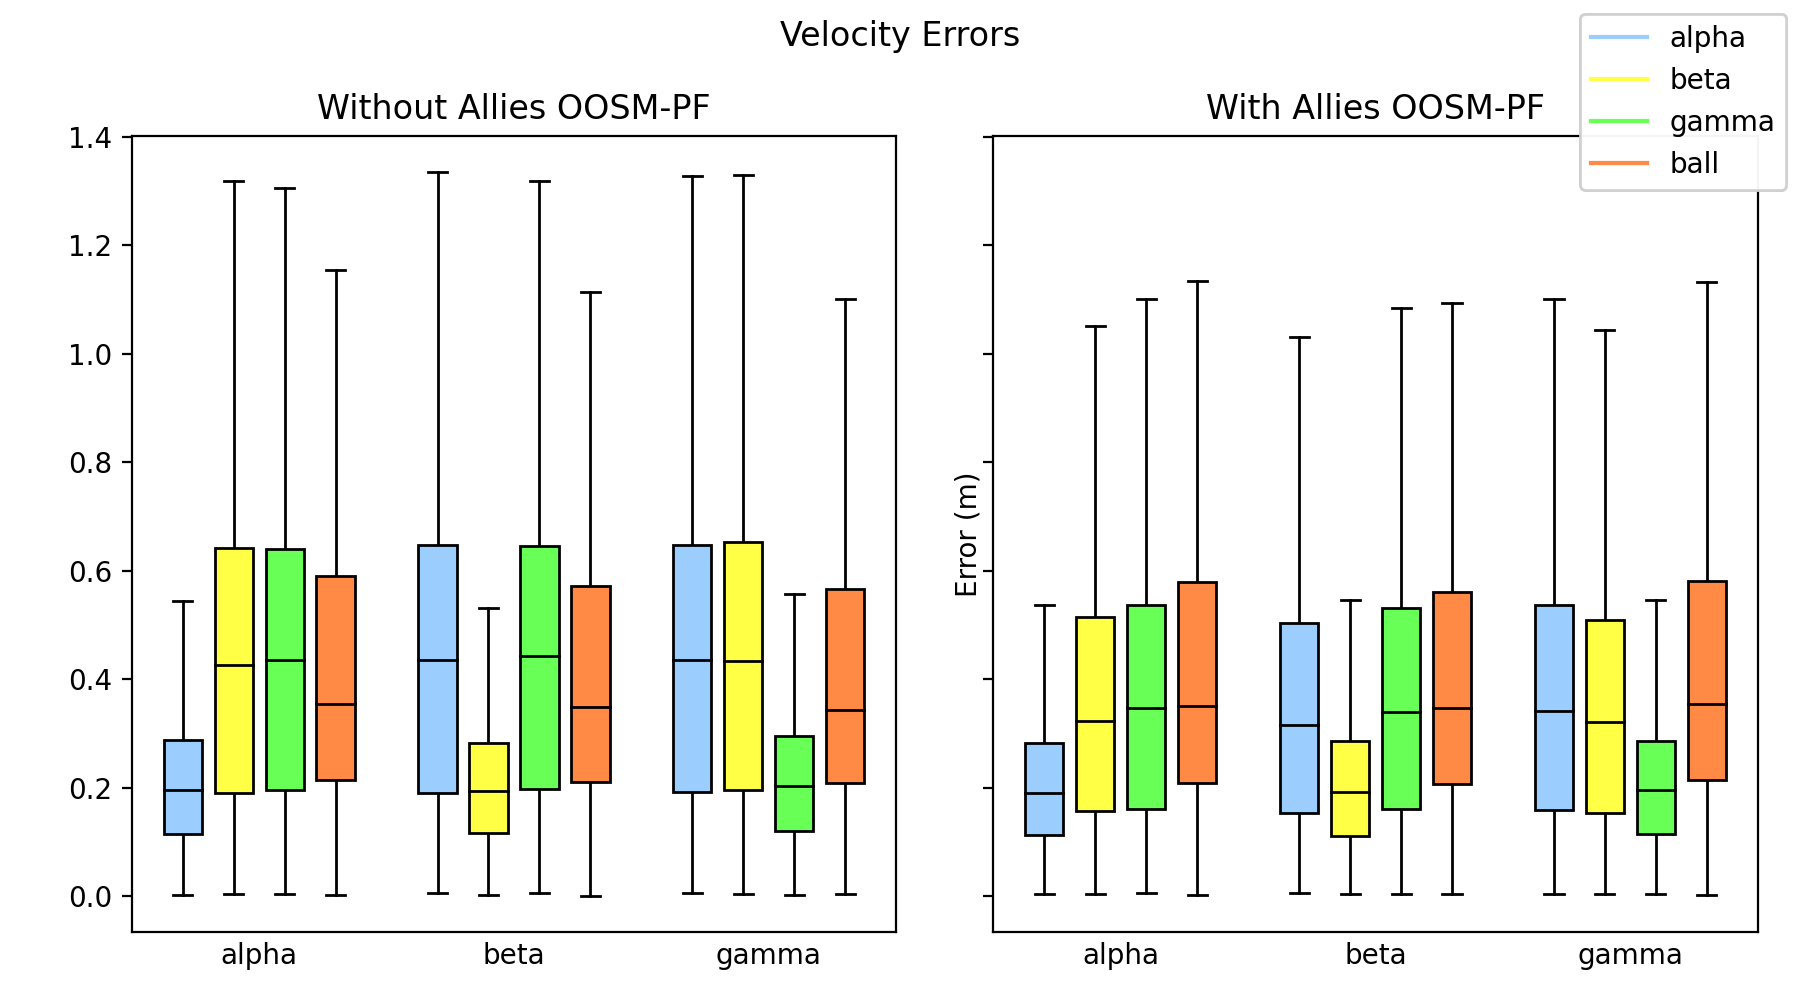
\includegraphics[width=0.9\textwidth]{resources/cfg3_AS_AT_error_vel.png}
    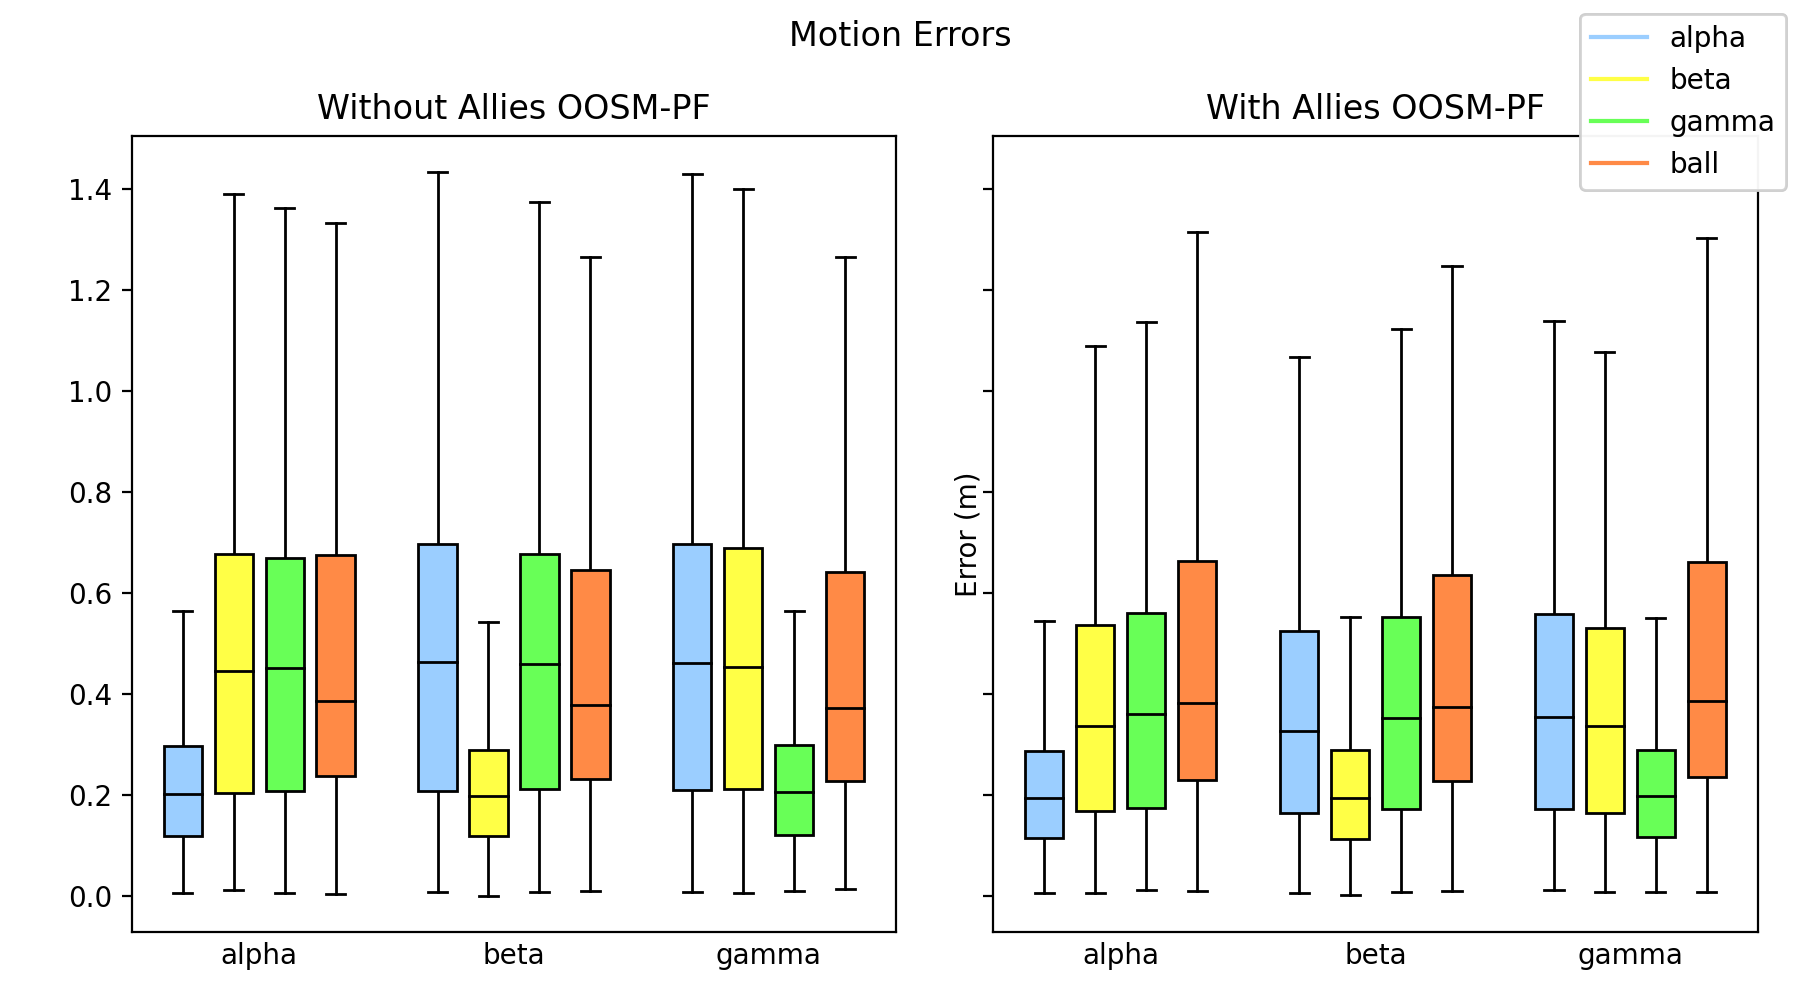
\includegraphics[width=0.9\textwidth]{resources/cfg3_AS_AT_error_motion.png}
    \caption{\textit{Error} \textit{world model} S dan T jaringan buruk}
    \label{fig:3-s-t-error}
    \bigskip
\end{figure}

Pada grafik \ref{fig:1-s-t-error}, hasil estimasi posisi dan kecepatan dari robot teman sedikit memburuk. Hal ini dikarenakan hasil persepsi \textit{vision} yang lebih \textit{noisy} dibandingkan dengan hasil lokalisasi yang menggunakan beberapa sensor berbeda. Sedangkan pada grafik \ref{fig:2-s-t-error} dan \ref{fig:3-s-t-error}, koreksi robot teman dapat membantu meningkatkan akurasi estimasi posisi dan kecepatan karena persepsi \textit{vision} yang lebih tersedia dibandingkan menunggu informasi dari robot teman yang terlambat.
